\documentclass[12pt,a4paper]{article}
\usepackage[utf8]{inputenc}
\usepackage[T1]{fontenc}
\usepackage[italian]{babel}
\usepackage{graphicx}
\usepackage{float}
\usepackage{geometry}
\usepackage{caption}
\usepackage{array}
\usepackage{longtable}
\usepackage{booktabs}
\usepackage{enumitem}
\usepackage{hyperref}
\usepackage{titlesec}
\usepackage{fancyhdr}
\usepackage{xcolor}
\usepackage{url}

\geometry{
    left=2.5cm,
    right=2.5cm,
    top=2.5cm,
    bottom=2.5cm
}

\hypersetup{
    colorlinks=true,
    linkcolor=blue!60!black,
    urlcolor=blue!60!black,
}

\setlength{\headheight}{14.5pt}
\addtolength{\topmargin}{-2.5pt}
\pagestyle{fancy}
\fancyhf{}
\rhead{BugBoard26 --- Specifica dei Requisiti Software}
\lhead{\thepage}
\renewcommand{\headrulewidth}{0.4pt}

% ============================================================
\begin{document}
% ============================================================

% --- Frontespizio ---
\begin{titlepage}
    \centering
    \vspace*{2cm}
    {\LARGE \textbf{Università degli Studi di Napoli Federico II}} \\[0.5cm]
    {\large Corso di Ingegneria del Software --- Canale 2} \\[3cm]

    \rule{\linewidth}{0.5mm} \\[0.4cm]
    {\Huge \textbf{BugBoard26}} \\[0.2cm]
    {\Large Documento di Specifica dei Requisiti Software (SRS)} \\
    \rule{\linewidth}{0.5mm} \\[2cm]

    {\large
    \begin{tabular}{ll}
        \textbf{Versione:} & 2.0 \\[0.3cm]
        \textbf{Data:}     & \today \\[0.3cm]
        \textbf{Stato:}    & Consegna progetto completo \\
    \end{tabular}
    } \\[3cm]

    \vfill
    {\large Anno Accademico 2025/2026}
\end{titlepage}

% --- Indice ---
\tableofcontents
\newpage

% ============================================================
\section{Introduzione}
% ============================================================

\subsection{Scopo del documento}
Il presente documento costituisce la Specifica dei Requisiti Software (SRS) per il sistema \textbf{BugBoard26}, sviluppato nell'ambito del corso di Ingegneria del Software. Il documento descrive le funzionalità del sistema, i suoi attori, i casi d'uso formalizzati, i requisiti non funzionali e fornisce una prima prototipazione visuale dell'interfaccia utente.

\subsection{Descrizione del sistema}
BugBoard26 è un'applicazione web per il \textbf{tracciamento e la gestione collaborativa di segnalazioni di bug}. Il sistema consente a team di sviluppo di:
\begin{itemize}
    \item segnalare bug, feature request e miglioramenti;
    \item assegnare le segnalazioni agli sviluppatori;
    \item tracciare il ciclo di vita di ogni segnalazione (apertura, presa in carico, risoluzione, archiviazione);
    \item aggiungere commenti e allegati fotografici;
    \item visualizzare statistiche e generare report mensili sull'attività del team.
\end{itemize}

\subsection{Riferimenti}
\begin{itemize}
    \item A. Cockburn, \textit{Writing Effective Use Cases}, Addison-Wesley, 2001
    \item Traccia progetto corso Ingegneria del Software --- Canale 2
    \item Documentazione di riferimento: DietiDeals24 (esempio fornito dal docente)
\end{itemize}

% ============================================================
% GLOSSARIO
% ============================================================
% GLOSSARIO - BugBoard26
% Includere con % ============================================================
% GLOSSARIO - BugBoard26
% Includere con % ============================================================
% GLOSSARIO - BugBoard26
% Includere con \input{glossario}
% ============================================================

\section{Glossario}

Di seguito sono riportati i termini tecnici e di dominio utilizzati nel presente documento e nel sistema BugBoard26.

\begin{description}[style=nextline, leftmargin=3cm, labelwidth=2.8cm]

    \item[Admin]
    Utente con privilegi amministrativi completi. Può gestire utenti, accedere a tutti i bug del sistema, generare report e modificare configurazioni.

    \item[Allegato]
    File immagine (JPEG, PNG, GIF, WebP, dimensione massima 5\,MB) caricato in associazione a un bug per documentarne visivamente il problema o la soluzione.

    \item[Archiviazione]
    Operazione che sposta un bug in stato \textit{Archived}, rimuovendolo dalla lista attiva senza eliminarlo definitivamente dal sistema.

    \item[Assegnatario]
    Utente registrato responsabile della risoluzione di un determinato bug.

    \item[Bug]
    Segnalazione di un comportamento anomalo, errato o inatteso di un sistema software. Nel contesto di BugBoard26 il termine indica genericamente qualsiasi segnalazione inserita nel sistema, indipendentemente dal tipo (Bug, Feature, Enhancement).

    \item[BugBoard26]
    Il sistema software oggetto di questo documento. Applicazione web per il tracciamento e la gestione collaborativa delle segnalazioni di bug.

    \item[Caso d'uso]
    Descrizione di un'interazione tra un attore e il sistema per raggiungere un obiettivo specifico. Formalizzato secondo il metodo di Alistair Cockburn.

    \item[Commento]
    Testo inserito da un utente in associazione a un bug per fornire aggiornamenti, chiarimenti o informazioni aggiuntive.

    \item[Docker]
    Piattaforma di containerizzazione utilizzata per impacchettare e distribuire i componenti dell'applicazione (frontend e backend) in modo indipendente dall'ambiente host.

    \item[Enhancement]
    Tipo di segnalazione che indica una richiesta di miglioramento di una funzionalità già esistente. Distinto da un Bug (errore) e da una Feature (nuova funzionalità).

    \item[Feature]
    Tipo di segnalazione che indica la richiesta di implementazione di una nuova funzionalità nel sistema.

    \item[History (Storico)]
    Registro cronologico di tutte le modifiche apportate a un bug nel tempo: cambi di stato, assegnazioni, commenti, aggiunta di allegati.

    \item[JWT (JSON Web Token)]
    Standard aperto (RFC 7519) utilizzato per autenticare in modo sicuro le richieste HTTP tra frontend e backend. Il token viene generato al login e incluso in ogni richiesta successiva.

    \item[Label]
    Etichetta testuale opzionale associabile a un bug per categorizzarlo ulteriormente (es.\ ``frontend'', ``performance'', ``regression'').

    \item[Priorità]
    Livello di urgenza di un bug. I valori previsti sono: \textit{Low}, \textit{Medium}, \textit{High}, \textit{Critical}.

    \item[ReadOnly (Utente)]
    Ruolo con accesso in sola lettura. L'utente ReadOnly può visualizzare bug, commenti e allegati, ma non può creare, modificare o commentare.

    \item[Report Mensile]
    Documento generato dal sistema contenente statistiche aggregate sull'attività del periodo selezionato: numero di bug creati, risolti, tempo medio di risoluzione, distribuzione per priorità e tipo.

    \item[Ruolo]
    Insieme di permessi associato a un utente. I ruoli previsti sono: \textit{USER} (utente standard), \textit{READONLY} (sola lettura), \textit{ADMIN} (amministratore).

    \item[Stato (Status)]
    Fase del ciclo di vita di un bug. Gli stati previsti sono:
    \begin{itemize}
        \item \textit{Todo}: bug appena creato, non ancora preso in carico
        \item \textit{In Progress}: bug in fase di risoluzione
        \item \textit{Resolved}: bug risolto
        \item \textit{Archived}: bug archiviato
    \end{itemize}

    \item[Tipo (Type)]
    Categoria della segnalazione. I valori previsti sono: \textit{Bug}, \textit{Feature}, \textit{Enhancement}.

    \item[USER (Utente registrato)]
    Ruolo standard. L'utente può creare bug, commentare, caricare allegati, assegnare bug (se Admin) e gestire il proprio profilo.

\end{description}

% ============================================================

\section{Glossario}

Di seguito sono riportati i termini tecnici e di dominio utilizzati nel presente documento e nel sistema BugBoard26.

\begin{description}[style=nextline, leftmargin=3cm, labelwidth=2.8cm]

    \item[Admin]
    Utente con privilegi amministrativi completi. Può gestire utenti, accedere a tutti i bug del sistema, generare report e modificare configurazioni.

    \item[Allegato]
    File immagine (JPEG, PNG, GIF, WebP, dimensione massima 5\,MB) caricato in associazione a un bug per documentarne visivamente il problema o la soluzione.

    \item[Archiviazione]
    Operazione che sposta un bug in stato \textit{Archived}, rimuovendolo dalla lista attiva senza eliminarlo definitivamente dal sistema.

    \item[Assegnatario]
    Utente registrato responsabile della risoluzione di un determinato bug.

    \item[Bug]
    Segnalazione di un comportamento anomalo, errato o inatteso di un sistema software. Nel contesto di BugBoard26 il termine indica genericamente qualsiasi segnalazione inserita nel sistema, indipendentemente dal tipo (Bug, Feature, Enhancement).

    \item[BugBoard26]
    Il sistema software oggetto di questo documento. Applicazione web per il tracciamento e la gestione collaborativa delle segnalazioni di bug.

    \item[Caso d'uso]
    Descrizione di un'interazione tra un attore e il sistema per raggiungere un obiettivo specifico. Formalizzato secondo il metodo di Alistair Cockburn.

    \item[Commento]
    Testo inserito da un utente in associazione a un bug per fornire aggiornamenti, chiarimenti o informazioni aggiuntive.

    \item[Docker]
    Piattaforma di containerizzazione utilizzata per impacchettare e distribuire i componenti dell'applicazione (frontend e backend) in modo indipendente dall'ambiente host.

    \item[Enhancement]
    Tipo di segnalazione che indica una richiesta di miglioramento di una funzionalità già esistente. Distinto da un Bug (errore) e da una Feature (nuova funzionalità).

    \item[Feature]
    Tipo di segnalazione che indica la richiesta di implementazione di una nuova funzionalità nel sistema.

    \item[History (Storico)]
    Registro cronologico di tutte le modifiche apportate a un bug nel tempo: cambi di stato, assegnazioni, commenti, aggiunta di allegati.

    \item[JWT (JSON Web Token)]
    Standard aperto (RFC 7519) utilizzato per autenticare in modo sicuro le richieste HTTP tra frontend e backend. Il token viene generato al login e incluso in ogni richiesta successiva.

    \item[Label]
    Etichetta testuale opzionale associabile a un bug per categorizzarlo ulteriormente (es.\ ``frontend'', ``performance'', ``regression'').

    \item[Priorità]
    Livello di urgenza di un bug. I valori previsti sono: \textit{Low}, \textit{Medium}, \textit{High}, \textit{Critical}.

    \item[ReadOnly (Utente)]
    Ruolo con accesso in sola lettura. L'utente ReadOnly può visualizzare bug, commenti e allegati, ma non può creare, modificare o commentare.

    \item[Report Mensile]
    Documento generato dal sistema contenente statistiche aggregate sull'attività del periodo selezionato: numero di bug creati, risolti, tempo medio di risoluzione, distribuzione per priorità e tipo.

    \item[Ruolo]
    Insieme di permessi associato a un utente. I ruoli previsti sono: \textit{USER} (utente standard), \textit{READONLY} (sola lettura), \textit{ADMIN} (amministratore).

    \item[Stato (Status)]
    Fase del ciclo di vita di un bug. Gli stati previsti sono:
    \begin{itemize}
        \item \textit{Todo}: bug appena creato, non ancora preso in carico
        \item \textit{In Progress}: bug in fase di risoluzione
        \item \textit{Resolved}: bug risolto
        \item \textit{Archived}: bug archiviato
    \end{itemize}

    \item[Tipo (Type)]
    Categoria della segnalazione. I valori previsti sono: \textit{Bug}, \textit{Feature}, \textit{Enhancement}.

    \item[USER (Utente registrato)]
    Ruolo standard. L'utente può creare bug, commentare, caricare allegati, assegnare bug (se Admin) e gestire il proprio profilo.

\end{description}

% ============================================================

\section{Glossario}

Di seguito sono riportati i termini tecnici e di dominio utilizzati nel presente documento e nel sistema BugBoard26.

\begin{description}[style=nextline, leftmargin=3cm, labelwidth=2.8cm]

    \item[Admin]
    Utente con privilegi amministrativi completi. Può gestire utenti, accedere a tutti i bug del sistema, generare report e modificare configurazioni.

    \item[Allegato]
    File immagine (JPEG, PNG, GIF, WebP, dimensione massima 5\,MB) caricato in associazione a un bug per documentarne visivamente il problema o la soluzione.

    \item[Archiviazione]
    Operazione che sposta un bug in stato \textit{Archived}, rimuovendolo dalla lista attiva senza eliminarlo definitivamente dal sistema.

    \item[Assegnatario]
    Utente registrato responsabile della risoluzione di un determinato bug.

    \item[Bug]
    Segnalazione di un comportamento anomalo, errato o inatteso di un sistema software. Nel contesto di BugBoard26 il termine indica genericamente qualsiasi segnalazione inserita nel sistema, indipendentemente dal tipo (Bug, Feature, Enhancement).

    \item[BugBoard26]
    Il sistema software oggetto di questo documento. Applicazione web per il tracciamento e la gestione collaborativa delle segnalazioni di bug.

    \item[Caso d'uso]
    Descrizione di un'interazione tra un attore e il sistema per raggiungere un obiettivo specifico. Formalizzato secondo il metodo di Alistair Cockburn.

    \item[Commento]
    Testo inserito da un utente in associazione a un bug per fornire aggiornamenti, chiarimenti o informazioni aggiuntive.

    \item[Docker]
    Piattaforma di containerizzazione utilizzata per impacchettare e distribuire i componenti dell'applicazione (frontend e backend) in modo indipendente dall'ambiente host.

    \item[Enhancement]
    Tipo di segnalazione che indica una richiesta di miglioramento di una funzionalità già esistente. Distinto da un Bug (errore) e da una Feature (nuova funzionalità).

    \item[Feature]
    Tipo di segnalazione che indica la richiesta di implementazione di una nuova funzionalità nel sistema.

    \item[History (Storico)]
    Registro cronologico di tutte le modifiche apportate a un bug nel tempo: cambi di stato, assegnazioni, commenti, aggiunta di allegati.

    \item[JWT (JSON Web Token)]
    Standard aperto (RFC 7519) utilizzato per autenticare in modo sicuro le richieste HTTP tra frontend e backend. Il token viene generato al login e incluso in ogni richiesta successiva.

    \item[Label]
    Etichetta testuale opzionale associabile a un bug per categorizzarlo ulteriormente (es.\ ``frontend'', ``performance'', ``regression'').

    \item[Priorità]
    Livello di urgenza di un bug. I valori previsti sono: \textit{Low}, \textit{Medium}, \textit{High}, \textit{Critical}.

    \item[ReadOnly (Utente)]
    Ruolo con accesso in sola lettura. L'utente ReadOnly può visualizzare bug, commenti e allegati, ma non può creare, modificare o commentare.

    \item[Report Mensile]
    Documento generato dal sistema contenente statistiche aggregate sull'attività del periodo selezionato: numero di bug creati, risolti, tempo medio di risoluzione, distribuzione per priorità e tipo.

    \item[Ruolo]
    Insieme di permessi associato a un utente. I ruoli previsti sono: \textit{USER} (utente standard), \textit{READONLY} (sola lettura), \textit{ADMIN} (amministratore).

    \item[Stato (Status)]
    Fase del ciclo di vita di un bug. Gli stati previsti sono:
    \begin{itemize}
        \item \textit{Todo}: bug appena creato, non ancora preso in carico
        \item \textit{In Progress}: bug in fase di risoluzione
        \item \textit{Resolved}: bug risolto
        \item \textit{Archived}: bug archiviato
    \end{itemize}

    \item[Tipo (Type)]
    Categoria della segnalazione. I valori previsti sono: \textit{Bug}, \textit{Feature}, \textit{Enhancement}.

    \item[USER (Utente registrato)]
    Ruolo standard. L'utente può creare bug, commentare, caricare allegati, assegnare bug (se Admin) e gestire il proprio profilo.

\end{description}


% ============================================================
\section{Individuazione e caratterizzazione degli utenti (attori)}
% ============================================================

Il sistema prevede quattro tipologie di attori umani e un attore di sistema:

\begin{description}[style=nextline]
    \item[Utente non registrato (Guest)]
    Chiunque acceda all'applicazione senza credenziali. Può accedere alla pagina di login e di registrazione. Non ha accesso ad alcuna funzionalità interna.

    \item[Utente registrato (USER)]
    Utente autenticato con ruolo standard. Può creare e modificare bug, aggiungere commenti e allegati, visualizzare lo storico, gestire il proprio profilo.

    \item[Utente ReadOnly]
    Utente autenticato con accesso in sola lettura. Può visualizzare bug, commenti e allegati, ma non può eseguire operazioni di scrittura.

    \item[Admin]
    Utente con privilegi amministrativi completi. Eredita tutte le funzionalità di USER e può in aggiunta: gestire gli utenti del sistema, assegnare bug, visualizzare metriche, generare report, esportare dati.

    \item[Sistema]
    Attore non umano che esegue operazioni automatiche: invio di notifiche, generazione dello storico modifiche, validazione degli allegati.
\end{description}

% ============================================================
\section{Modellazione dei Casi d'Uso}
% ============================================================

\subsection{Tabella dei Casi d'Uso per Attore}
\section{Tabella dei Casi d'Uso}

\begin{longtable}{|p{3cm}|p{11cm}|}
\hline
\textbf{Attore} & \textbf{Casi d'uso} \\
\hline
\endfirsthead
\hline
\textbf{Attore} & \textbf{Casi d'uso} \\
\hline
\endhead
\hline
\endfoot
\hline
\endlastfoot

Utente non registrato &
\begin{itemize}[leftmargin=*,nosep,nolistsep]
    \item Registrazione al sistema tramite email
    \item Visualizzazione informazioni pubbliche dell'applicazione
    \item Accesso alla pagina di login
\end{itemize} \\
\hline

Utente registrato (USER) &
\begin{itemize}[leftmargin=*,nosep,nolistsep]
    \item Login/logout al sistema
    \item Visualizzazione lista bug con filtri (tipo, stato, priorità, label)
    \item Visualizzazione dettagli singolo bug
    \item Creazione nuovo bug
    \item Modifica bug propri o assegnati
    \item Aggiunta commenti ai bug
    \item Upload allegati immagini ai bug
    \item Assegnazione bug ad altri utenti
    \item Archiviazione bug risolti
    \item Marcatura bug come duplicati
    \item Visualizzazione storico modifiche bug
    \item Gestione profilo personale
    \item Cambio password
\end{itemize} \\
\hline

Utente ReadOnly &
\begin{itemize}[leftmargin=*,nosep,nolistsep]
    \item Login al sistema
    \item Visualizzazione lista bug con filtri
    \item Visualizzazione dettagli singolo bug
    \item Visualizzazione commenti e allegati
    \item Visualizzazione storico modifiche
    \item Visualizzazione profilo proprio (sola lettura)
\end{itemize} \\
\hline

Admin &
\begin{itemize}[leftmargin=*,nosep,nolistsep]
    \item Tutti i casi d'uso dell'Utente registrato
    \item Gestione completa utenti (visualizzazione, modifica ruoli, disabilitazione)
    \item Visualizzazione metriche di sistema
    \item Generazione report mensili
    \item Esportazione dati in formato Excel
    \item Accesso completo a tutti i bug del sistema
    \item Gestione label e categorie
    \item Configurazione parametri di sistema
\end{itemize} \\
\hline

Sistema &
\begin{itemize}[leftmargin=*,nosep,nolistsep]
    \item Invio notifiche automatiche su cambiamenti bug
    \item Archiviazione automatica bug dopo periodo di inattività
    \item Generazione automatica storico modifiche
    \item Validazione automatica allegati (tipo e dimensione)
    \item Pulizia automatica dati obsoleti
    \item Backup automatico dati
\end{itemize} \\
\hline
\caption{Tabella completa dei casi d'uso per BugBoard26}
\label{tab:casi_uso}
\end{longtable}

\subsection{Descrizione dettagliata dei casi d'uso}

\subsubsection{Utente non registrato}
\begin{itemize}
    \item \textbf{Registrazione al sistema tramite email}: L'utente può creare un nuovo account fornendo email, password e informazioni personali. Il sistema invia una email di conferma per verificare l'indirizzo.
    \item \textbf{Visualizzazione informazioni pubbliche}: Accesso alla pagina principale dell'applicazione con informazioni generali sul servizio di bug tracking.
    \item \textbf{Accesso alla pagina di login}: Possibilità di accedere al sistema utilizzando credenziali esistenti.
\end{itemize}

\subsubsection{Utente registrato (USER)}
\begin{itemize}
    \item \textbf{Login/logout al sistema}: Autenticazione tramite credenziali email/password con generazione di token JWT per sessioni sicure.
    \item \textbf{Visualizzazione lista bug con filtri}: Consultazione dell'elenco completo dei bug con possibilità di filtrare per tipo, stato, priorità, label e ricerca testuale.
    \item \textbf{Visualizzazione dettagli singolo bug}: Accesso completo alle informazioni di un bug specifico, inclusi descrizione, commenti, allegati e storico modifiche.
    \item \textbf{Creazione nuovo bug}: Inserimento di una nuova segnalazione con descrizione dettagliata, assegnazione priorità, tipo e label appropriate.
    \item \textbf{Modifica bug propri o assegnati}: Possibilità di aggiornare informazioni, stato e dettagli dei bug creati dall'utente o assegnati al suo account.
    \item \textbf{Aggiunta commenti ai bug}: Inserimento di commenti testuali per fornire aggiornamenti, soluzioni o richiedere chiarimenti.
    \item \textbf{Upload allegati immagini ai bug}: Caricamento di immagini (JPEG, PNG, GIF, WebP) fino a 5MB per documentare visivamente il problema.
    \item \textbf{Assegnazione bug ad altri utenti}: Trasferimento della responsabilità di un bug a un altro utente registrato nel sistema.
    \item \textbf{Archiviazione bug risolti}: Spostamento dei bug risolti in stato archiviato per mantenere pulita la lista attiva.
    \item \textbf{Marcatura bug come duplicati}: Collegamento di un bug a un altro esistente quando viene identificato come duplicato.
    \item \textbf{Visualizzazione storico modifiche bug}: Consultazione cronologica di tutte le modifiche apportate a un bug nel tempo.
    \item \textbf{Gestione profilo personale}: Modifica delle informazioni personali, preferenze e impostazioni dell'account.
    \item \textbf{Cambio password}: Aggiornamento della password di accesso con validazione di sicurezza.
\end{itemize}

\subsubsection{Utente ReadOnly}
\begin{itemize}
    \item \textbf{Login al sistema}: Accesso con credenziali per utenti con privilegi di sola lettura.
    \item \textbf{Visualizzazione lista bug con filtri}: Consultazione dell'elenco bug con possibilità di applicare filtri di ricerca.
    \item \textbf{Visualizzazione dettagli singolo bug}: Accesso in sola lettura alle informazioni complete di un bug.
    \item \textbf{Visualizzazione commenti e allegati}: Lettura di tutti i commenti e download/visualizzazione degli allegati associati.
    \item \textbf{Visualizzazione storico modifiche}: Consultazione della cronologia delle modifiche senza possibilità di intervento.
    \item \textbf{Visualizzazione profilo proprio}: Accesso limitato alle informazioni del proprio profilo utente.
\end{itemize}

\subsubsection{Admin}
\begin{itemize}
    \item \textbf{Tutti i casi d'uso dell'Utente registrato}: L'amministratore eredita tutte le funzionalità dell'utente standard.
    \item \textbf{Gestione completa utenti}: Creazione, modifica, disabilitazione e gestione ruoli degli utenti del sistema.
    \item \textbf{Visualizzazione metriche di sistema}: Accesso a dashboard con statistiche, grafici e KPI del sistema.
    \item \textbf{Generazione report mensili}: Creazione di report dettagliati sull'attività del sistema per periodo specificato.
    \item \textbf{Esportazione dati in formato Excel}: Estrazione completa dei dati in formato spreadsheet per analisi esterne.
    \item \textbf{Accesso completo a tutti i bug}: Possibilità di visualizzare e modificare qualsiasi bug del sistema indipendentemente dall'assegnazione.
    \item \textbf{Gestione label e categorie}: Creazione, modifica ed eliminazione delle etichette e categorie di classificazione.
    \item \textbf{Configurazione parametri di sistema}: Modifica delle impostazioni globali, limiti e comportamenti dell'applicazione.
\end{itemize}

\subsubsection{Sistema}
\begin{itemize}
    \item \textbf{Invio notifiche automatiche}: Meccanismo automatico di notifica via email o push per aggiornamenti sui bug seguiti.
    \item \textbf{Archiviazione automatica}: Processo schedulato per archiviare automaticamente bug inattivi dopo un periodo configurabile.
    \item \textbf{Generazione automatica storico}: Registrazione automatica di ogni modifica apportata ai bug nel database.
    \item \textbf{Validazione automatica allegati}: Controllo automatico di tipo, dimensione e sicurezza dei file caricati.
    \item \textbf{Pulizia automatica dati obsoleti}: Eliminazione periodica di dati temporanei, cache e informazioni non più necessarie.
    \item \textbf{Backup automatico dati}: Salvataggio automatico periodico del database e dei file allegati per disaster recovery.
\end{itemize}



\subsection{Diagrammi UML dei Casi d'Uso}

\subsubsection{Diagramma Generale del Sistema}
\begin{figure}[H]
    \centering
    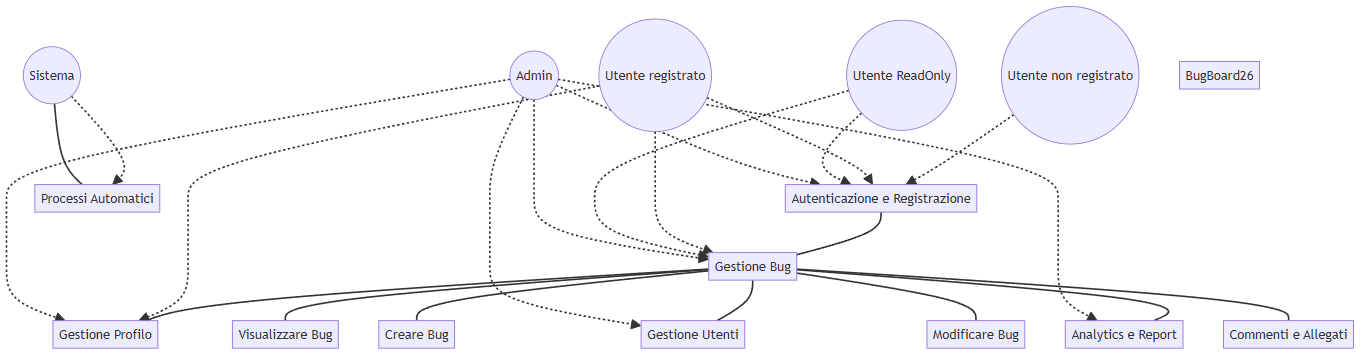
\includegraphics[width=0.85\textwidth]{immagini/diagramma_generale.png}
    \caption{Diagramma generale dei casi d'uso --- BugBoard26}
    \label{fig:uc_generale}
\end{figure}

\subsubsection{Diagramma Dettagliato --- Gestione Bug}
\begin{figure}[H]
    \centering
    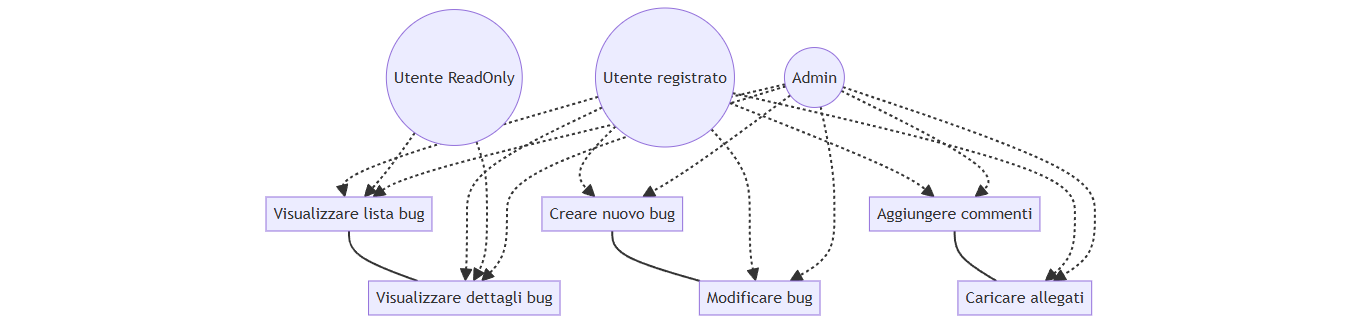
\includegraphics[width=0.85\textwidth]{immagini/diagramma_bug_management.png}
    \caption{Diagramma dettagliato --- Gestione Bug}
    \label{fig:uc_bug}
\end{figure}

\subsubsection{Diagramma Dettagliato --- Amministrazione}
\begin{figure}[H]
    \centering
    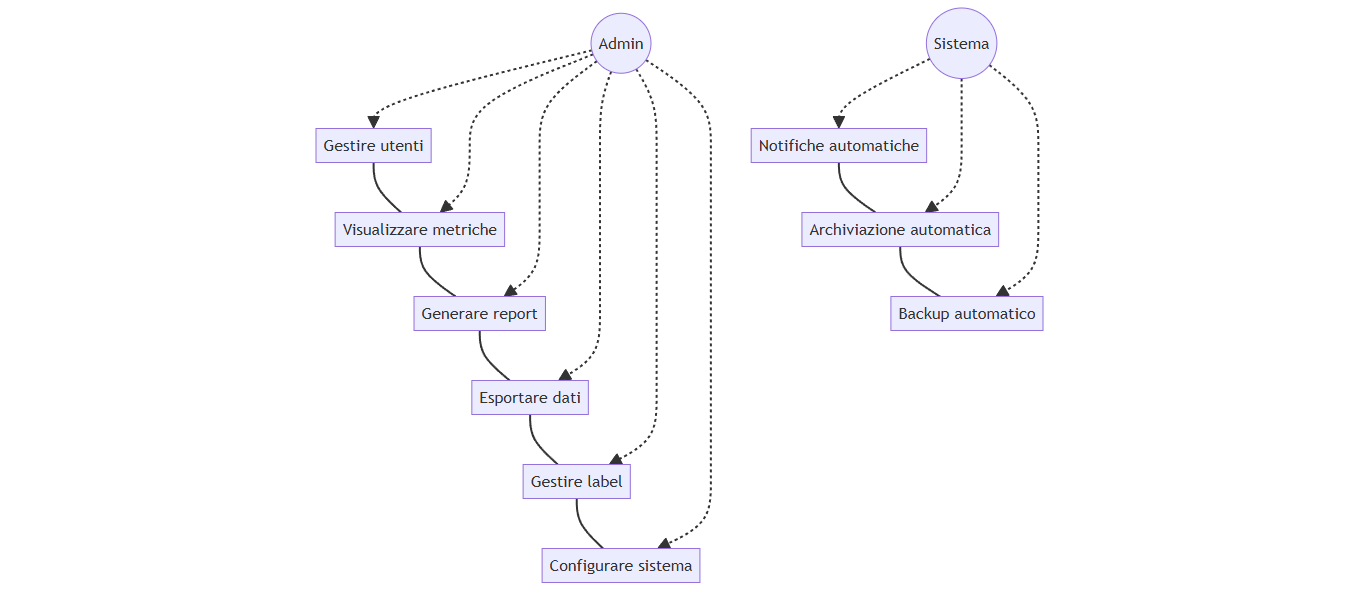
\includegraphics[width=0.85\textwidth]{immagini/diagramma_amministrazione.png}
    \caption{Diagramma dettagliato --- Amministrazione e funzioni di sistema}
    \label{fig:uc_admin}
\end{figure}

\subsection{Convenzioni grafiche}
\begin{itemize}
    \item \textbf{Attori} (omino stilizzato o rettangolo): entità esterne che interagiscono con il sistema
    \item \textbf{Casi d'uso} (ellissi): funzionalità offerte dal sistema
    \item \textbf{Linee solide}: relazione di associazione tra attore e caso d'uso
    \item \textbf{Frecce tratteggiate $\ll$include$\gg$}: il caso d'uso base include sempre il caso d'uso puntato
    \item \textbf{Frecce tratteggiate $\ll$extend$\gg$}: il caso d'uso puntato estende opzionalmente il caso d'uso base
\end{itemize}

% ============================================================
\section{Formalizzazione dei Casi d'Uso (Cockburn)}
% ============================================================

In questa sezione vengono formalizzati quattro casi d'uso significativi, secondo il formalismo tabellare di Alistair Cockburn. Sono stati esclusi i casi d'uso relativi a registrazione e autenticazione, come indicato nelle istruzioni della traccia.

% ============================================================
% CORPO: Casi d'Uso Dettagliati (Formalismo Cockburn)
% Questo file va incluso con % ============================================================
% CORPO: Casi d'Uso Dettagliati (Formalismo Cockburn)
% Questo file va incluso con % ============================================================
% CORPO: Casi d'Uso Dettagliati (Formalismo Cockburn)
% Questo file va incluso con \input{casi_uso_dettagliati_body}
% ============================================================

\subsection{Caso d'Uso 1: Creazione nuovo bug}

\begin{longtable}{|p{3cm}|p{7cm}|p{5.5cm}|}
\hline
\textbf{Campo} & \multicolumn{2}{p{12.5cm}|}{\textbf{Descrizione}} \\
\hline
\endfirsthead
\hline
\textbf{Campo} & \multicolumn{2}{p{12.5cm}|}{\textbf{Descrizione}} \\
\hline
\endhead
\hline
\endfoot
\hline
\endlastfoot

USE CASE \#01 & \multicolumn{2}{p{12.5cm}|}{CREAZIONE NUOVO BUG} \\
\hline
Goal & \multicolumn{2}{p{12.5cm}|}{L'utente vuole segnalare un nuovo bug nel sistema} \\
\hline
Preconditions & \multicolumn{2}{p{12.5cm}|}{L'utente deve essere autenticato (ruolo USER o ADMIN)} \\
\hline
Success End Condition & \multicolumn{2}{p{12.5cm}|}{Il bug è creato con successo e registrato con un ID univoco} \\
\hline
Failed End Condition & \multicolumn{2}{p{12.5cm}|}{Il bug non viene creato a causa di errori di validazione o problemi di sistema} \\
\hline
Primary Actor & \multicolumn{2}{p{12.5cm}|}{Utente registrato (USER)} \\
\hline\hline
\textbf{DESCRIPTION} & \textbf{Utente} & \textbf{Sistema} \\
\hline
Step 1 & Accede alla sezione ``Nuovo Bug'' & Mostra il form con i campi obbligatori \\
\hline
Step 2 & Inserisce il titolo del bug & Valida che il titolo non sia vuoto \\
\hline
Step 3 & Seleziona il tipo (Bug, Feature, Enhancement) & Carica le categorie disponibili \\
\hline
Step 4 & Inserisce la descrizione dettagliata & Fornisce un'area di testo \\
\hline
Step 5 & Seleziona la priorità (Low, Medium, High, Critical) & Mostra le opzioni con colori identificativi \\
\hline
Step 6 & Aggiunge label/tag opzionali & Permette selezione multipla da lista \\
\hline
Step 7 & Carica immagini allegati (opzionale) & Valida formato (JPEG, PNG, GIF, WebP) e dimensione (max 5\,MB) \\
\hline
Step 8 & Seleziona assegnatario (opzionale) & Mostra lista utenti attivi \\
\hline
Step 9 & Clicca su ``Crea Bug'' & Valida tutti i campi obbligatori \\
\hline
Step 10 & & Salva il bug nel database \\
\hline
Step 11 & & Invia notifica all'utente assegnato (se presente) \\
\hline
Step 12 & & Mostra conferma con l'ID del bug creato \\
\hline\hline
\textbf{EXTENSIONS} & \textbf{Step} & \textbf{Descrizione} \\
\hline
Caricamento immagini fallito & 7.a & Mostra errore ``Formato non supportato'' \\
\hline
 & 7.b & L'utente può riprovare con file diverso \\
\hline
Validazione campi fallita & 9.a & Evidenzia i campi con errori \\
\hline
 & 9.b & Mostra messaggi di errore per ciascun campo \\
\hline
Utente assegnatario non trovato & 8.a & Mostra errore ``Utente non trovato'' \\
\hline
 & 8.b & L'utente può eseguire una nuova ricerca \\
\hline
\end{longtable}

% ============================================================
\subsection{Caso d'Uso 2: Assegnazione bug a un utente}

\begin{longtable}{|p{3cm}|p{7cm}|p{5.5cm}|}
\hline
\textbf{Campo} & \multicolumn{2}{p{12.5cm}|}{\textbf{Descrizione}} \\
\hline
\endfirsthead
\hline
\textbf{Campo} & \multicolumn{2}{p{12.5cm}|}{\textbf{Descrizione}} \\
\hline
\endhead
\hline
\endfoot
\hline
\endlastfoot

USE CASE \#02 & \multicolumn{2}{p{12.5cm}|}{ASSEGNAZIONE BUG A UN UTENTE} \\
\hline
Goal & \multicolumn{2}{p{12.5cm}|}{L'amministratore vuole assegnare o riassegnare un bug a un utente del sistema} \\
\hline
Preconditions & \multicolumn{2}{p{12.5cm}|}{L'utente deve essere autenticato con ruolo ADMIN; il bug deve esistere nel sistema} \\
\hline
Success End Condition & \multicolumn{2}{p{12.5cm}|}{Il bug risulta assegnato al nuovo utente e la modifica è registrata nello storico} \\
\hline
Failed End Condition & \multicolumn{2}{p{12.5cm}|}{L'assegnazione fallisce per utente di destinazione non valido} \\
\hline
Primary Actor & \multicolumn{2}{p{12.5cm}|}{Admin} \\
\hline\hline
\textbf{DESCRIPTION} & \textbf{Utente (Admin)} & \textbf{Sistema} \\
\hline
Step 1 & Visualizza i dettagli di un bug & Mostra la pagina di dettaglio con tutte le informazioni \\
\hline
Step 2 & Clicca su ``Assegna'' & Apre il form di assegnazione \\
\hline
Step 3 & Inserisce email o nome del nuovo assegnatario & Fornisce autocomplete con ricerca utenti \\
\hline
Step 4 & Seleziona l'utente dalla lista & Valida che l'utente esista e sia attivo \\
\hline
Step 5 & Aggiunge una nota (opzionale) & Fornisce un campo testo per la motivazione \\
\hline
Step 6 & Clicca su ``Conferma Assegnazione'' & Verifica i permessi dell'utente richiedente \\
\hline
Step 7 & & Aggiorna il campo ``assegnato a'' nel database \\
\hline
Step 8 & & Registra la modifica nella tabella history \\
\hline
Step 9 & & Invia notifica al nuovo assegnatario \\
\hline
Step 10 & & Invia notifica all'assegnatario precedente (se diverso) \\
\hline
Step 11 & & Mostra messaggio di conferma \\
\hline\hline
\textbf{EXTENSIONS} & \textbf{Step} & \textbf{Descrizione} \\
\hline
Utente non trovato & 4.a & Mostra errore ``Utente non esistente'' \\
\hline
 & 4.b & L'admin può eseguire una nuova ricerca \\
\hline
Bug già assegnato & 6.a & Chiede conferma per il cambio di assegnazione \\
\hline
 & 6.b & Se confermato, procede con la riassegnazione \\
\hline
\end{longtable}

% ============================================================
\subsection{Caso d'Uso 3: Risoluzione e chiusura bug}

\begin{longtable}{|p{3cm}|p{7cm}|p{5.5cm}|}
\hline
\textbf{Campo} & \multicolumn{2}{p{12.5cm}|}{\textbf{Descrizione}} \\
\hline
\endfirsthead
\hline
\textbf{Campo} & \multicolumn{2}{p{12.5cm}|}{\textbf{Descrizione}} \\
\hline
\endhead
\hline
\endfoot
\hline
\endlastfoot

USE CASE \#03 & \multicolumn{2}{p{12.5cm}|}{RISOLUZIONE E CHIUSURA BUG} \\
\hline
Goal & \multicolumn{2}{p{12.5cm}|}{L'utente vuole marcare un bug come risolto} \\
\hline
Preconditions & \multicolumn{2}{p{12.5cm}|}{L'utente deve essere autenticato e assegnatario del bug; il bug deve essere in stato \textit{In Progress}} \\
\hline
Success End Condition & \multicolumn{2}{p{12.5cm}|}{Il bug viene aggiornato allo stato \textit{Resolved} con data di risoluzione registrata} \\
\hline
Failed End Condition & \multicolumn{2}{p{12.5cm}|}{La risoluzione fallisce per permessi insufficienti o stato del bug non valido} \\
\hline
Primary Actor & \multicolumn{2}{p{12.5cm}|}{Utente registrato (USER) assegnato al bug} \\
\hline\hline
\textbf{DESCRIPTION} & \textbf{Utente} & \textbf{Sistema} \\
\hline
Step 1 & Visualizza i dettagli del bug assegnato & Mostra la pagina di dettaglio con lo stato attuale \\
\hline
Step 2 & Clicca su ``Risolvi Bug'' & Verifica che il bug sia in stato \textit{In Progress} \\
\hline
Step 3 & & Mostra il form di risoluzione \\
\hline
Step 4 & Seleziona il tipo di risoluzione & Mostra opzioni: \textit{Fixed, Won't Fix, Duplicate, Cannot Reproduce} \\
\hline
Step 5 & Inserisce la descrizione della soluzione adottata & Fornisce un'area di testo \\
\hline
Step 6 & Carica immagini di conferma (opzionale) & Valida formato e dimensione degli allegati \\
\hline
Step 7 & Clicca su ``Conferma Risoluzione'' & Valida tutti i campi obbligatori \\
\hline
Step 8 & & Aggiorna lo stato a \textit{Resolved} \\
\hline
Step 9 & & Registra la data di risoluzione \\
\hline
Step 10 & & Crea un record nella tabella history \\
\hline
Step 11 & & Invia notifiche al creatore e ai follower del bug \\
\hline
Step 12 & & Mostra la pagina aggiornata con il nuovo stato \\
\hline\hline
\textbf{EXTENSIONS} & \textbf{Step} & \textbf{Descrizione} \\
\hline
Bug non in stato corretto & 2.a & Mostra ``Bug non può essere risolto in questo stato'' \\
\hline
 & 2.b & Suggerisce azioni alternative disponibili \\
\hline
Tipo risoluzione ``Duplicate'' & 4.a & Richiede la selezione del bug padre \\
\hline
 & 4.b & Crea automaticamente la relazione di duplicazione \\
\hline
Caricamento immagini fallito & 6.a & Mostra errore di formato o dimensione \\
\hline
 & 6.b & L'utente può proseguire senza allegati \\
\hline
\end{longtable}

% ============================================================
\subsection{Caso d'Uso 4: Generazione report mensile (Admin)}

\begin{longtable}{|p{3cm}|p{7cm}|p{5.5cm}|}
\hline
\textbf{Campo} & \multicolumn{2}{p{12.5cm}|}{\textbf{Descrizione}} \\
\hline
\endfirsthead
\hline
\textbf{Campo} & \multicolumn{2}{p{12.5cm}|}{\textbf{Descrizione}} \\
\hline
\endhead
\hline
\endfoot
\hline
\endlastfoot

USE CASE \#04 & \multicolumn{2}{p{12.5cm}|}{GENERAZIONE REPORT MENSILE} \\
\hline
Goal & \multicolumn{2}{p{12.5cm}|}{L'amministratore vuole generare un report sull'attività del sistema per un mese specifico} \\
\hline
Preconditions & \multicolumn{2}{p{12.5cm}|}{L'utente deve essere autenticato con ruolo ADMIN} \\
\hline
Success End Condition & \multicolumn{2}{p{12.5cm}|}{Il report viene generato e reso disponibile per il download} \\
\hline
Failed End Condition & \multicolumn{2}{p{12.5cm}|}{La generazione fallisce per assenza di dati nel periodo selezionato o errori di sistema} \\
\hline
Primary Actor & \multicolumn{2}{p{12.5cm}|}{Admin} \\
\hline\hline
\textbf{DESCRIPTION} & \textbf{Utente (Admin)} & \textbf{Sistema} \\
\hline
Step 1 & Accede alla sezione ``Analytics'' & Mostra la dashboard con le opzioni di reportistica \\
\hline
Step 2 & Seleziona ``Report Mensili'' & Carica la lista dei mesi disponibili \\
\hline
Step 3 & Seleziona mese e anno desiderati & Valida che il periodo esista e contenga dati \\
\hline
Step 4 & Clicca su ``Genera Report'' & Avvia il processo di generazione \\
\hline
Step 5 & & Raccoglie dati dalle tabelle bugs, users, history \\
\hline
Step 6 & & Calcola metriche: bug creati, risolti, tempo medio \\
\hline
Step 7 & & Genera grafici e statistiche aggregate \\
\hline
Step 8 & & Crea il documento in formato Excel \\
\hline
Step 9 & & Fornisce il link per il download \\
\hline
Step 10 & Scarica il report & Serve il file con nome che include il timestamp \\
\hline\hline
\textbf{EXTENSIONS} & \textbf{Step} & \textbf{Descrizione} \\
\hline
Mese senza dati & 3.a & Avvisa ``Nessun dato disponibile per il periodo selezionato'' \\
\hline
 & 3.b & Suggerisce periodi alternativi \\
\hline
Errore generazione & 8.a & Registra l'errore nel log \\
\hline
 & 8.b & Mostra un messaggio di errore all'amministratore \\
\hline
 & 8.c & Suggerisce di riprovare o contattare il supporto \\
\hline
\end{longtable}

% ============================================================

\subsection{Caso d'Uso 1: Creazione nuovo bug}

\begin{longtable}{|p{3cm}|p{7cm}|p{5.5cm}|}
\hline
\textbf{Campo} & \multicolumn{2}{p{12.5cm}|}{\textbf{Descrizione}} \\
\hline
\endfirsthead
\hline
\textbf{Campo} & \multicolumn{2}{p{12.5cm}|}{\textbf{Descrizione}} \\
\hline
\endhead
\hline
\endfoot
\hline
\endlastfoot

USE CASE \#01 & \multicolumn{2}{p{12.5cm}|}{CREAZIONE NUOVO BUG} \\
\hline
Goal & \multicolumn{2}{p{12.5cm}|}{L'utente vuole segnalare un nuovo bug nel sistema} \\
\hline
Preconditions & \multicolumn{2}{p{12.5cm}|}{L'utente deve essere autenticato (ruolo USER o ADMIN)} \\
\hline
Success End Condition & \multicolumn{2}{p{12.5cm}|}{Il bug è creato con successo e registrato con un ID univoco} \\
\hline
Failed End Condition & \multicolumn{2}{p{12.5cm}|}{Il bug non viene creato a causa di errori di validazione o problemi di sistema} \\
\hline
Primary Actor & \multicolumn{2}{p{12.5cm}|}{Utente registrato (USER)} \\
\hline\hline
\textbf{DESCRIPTION} & \textbf{Utente} & \textbf{Sistema} \\
\hline
Step 1 & Accede alla sezione ``Nuovo Bug'' & Mostra il form con i campi obbligatori \\
\hline
Step 2 & Inserisce il titolo del bug & Valida che il titolo non sia vuoto \\
\hline
Step 3 & Seleziona il tipo (Bug, Feature, Enhancement) & Carica le categorie disponibili \\
\hline
Step 4 & Inserisce la descrizione dettagliata & Fornisce un'area di testo \\
\hline
Step 5 & Seleziona la priorità (Low, Medium, High, Critical) & Mostra le opzioni con colori identificativi \\
\hline
Step 6 & Aggiunge label/tag opzionali & Permette selezione multipla da lista \\
\hline
Step 7 & Carica immagini allegati (opzionale) & Valida formato (JPEG, PNG, GIF, WebP) e dimensione (max 5\,MB) \\
\hline
Step 8 & Seleziona assegnatario (opzionale) & Mostra lista utenti attivi \\
\hline
Step 9 & Clicca su ``Crea Bug'' & Valida tutti i campi obbligatori \\
\hline
Step 10 & & Salva il bug nel database \\
\hline
Step 11 & & Invia notifica all'utente assegnato (se presente) \\
\hline
Step 12 & & Mostra conferma con l'ID del bug creato \\
\hline\hline
\textbf{EXTENSIONS} & \textbf{Step} & \textbf{Descrizione} \\
\hline
Caricamento immagini fallito & 7.a & Mostra errore ``Formato non supportato'' \\
\hline
 & 7.b & L'utente può riprovare con file diverso \\
\hline
Validazione campi fallita & 9.a & Evidenzia i campi con errori \\
\hline
 & 9.b & Mostra messaggi di errore per ciascun campo \\
\hline
Utente assegnatario non trovato & 8.a & Mostra errore ``Utente non trovato'' \\
\hline
 & 8.b & L'utente può eseguire una nuova ricerca \\
\hline
\end{longtable}

% ============================================================
\subsection{Caso d'Uso 2: Assegnazione bug a un utente}

\begin{longtable}{|p{3cm}|p{7cm}|p{5.5cm}|}
\hline
\textbf{Campo} & \multicolumn{2}{p{12.5cm}|}{\textbf{Descrizione}} \\
\hline
\endfirsthead
\hline
\textbf{Campo} & \multicolumn{2}{p{12.5cm}|}{\textbf{Descrizione}} \\
\hline
\endhead
\hline
\endfoot
\hline
\endlastfoot

USE CASE \#02 & \multicolumn{2}{p{12.5cm}|}{ASSEGNAZIONE BUG A UN UTENTE} \\
\hline
Goal & \multicolumn{2}{p{12.5cm}|}{L'amministratore vuole assegnare o riassegnare un bug a un utente del sistema} \\
\hline
Preconditions & \multicolumn{2}{p{12.5cm}|}{L'utente deve essere autenticato con ruolo ADMIN; il bug deve esistere nel sistema} \\
\hline
Success End Condition & \multicolumn{2}{p{12.5cm}|}{Il bug risulta assegnato al nuovo utente e la modifica è registrata nello storico} \\
\hline
Failed End Condition & \multicolumn{2}{p{12.5cm}|}{L'assegnazione fallisce per utente di destinazione non valido} \\
\hline
Primary Actor & \multicolumn{2}{p{12.5cm}|}{Admin} \\
\hline\hline
\textbf{DESCRIPTION} & \textbf{Utente (Admin)} & \textbf{Sistema} \\
\hline
Step 1 & Visualizza i dettagli di un bug & Mostra la pagina di dettaglio con tutte le informazioni \\
\hline
Step 2 & Clicca su ``Assegna'' & Apre il form di assegnazione \\
\hline
Step 3 & Inserisce email o nome del nuovo assegnatario & Fornisce autocomplete con ricerca utenti \\
\hline
Step 4 & Seleziona l'utente dalla lista & Valida che l'utente esista e sia attivo \\
\hline
Step 5 & Aggiunge una nota (opzionale) & Fornisce un campo testo per la motivazione \\
\hline
Step 6 & Clicca su ``Conferma Assegnazione'' & Verifica i permessi dell'utente richiedente \\
\hline
Step 7 & & Aggiorna il campo ``assegnato a'' nel database \\
\hline
Step 8 & & Registra la modifica nella tabella history \\
\hline
Step 9 & & Invia notifica al nuovo assegnatario \\
\hline
Step 10 & & Invia notifica all'assegnatario precedente (se diverso) \\
\hline
Step 11 & & Mostra messaggio di conferma \\
\hline\hline
\textbf{EXTENSIONS} & \textbf{Step} & \textbf{Descrizione} \\
\hline
Utente non trovato & 4.a & Mostra errore ``Utente non esistente'' \\
\hline
 & 4.b & L'admin può eseguire una nuova ricerca \\
\hline
Bug già assegnato & 6.a & Chiede conferma per il cambio di assegnazione \\
\hline
 & 6.b & Se confermato, procede con la riassegnazione \\
\hline
\end{longtable}

% ============================================================
\subsection{Caso d'Uso 3: Risoluzione e chiusura bug}

\begin{longtable}{|p{3cm}|p{7cm}|p{5.5cm}|}
\hline
\textbf{Campo} & \multicolumn{2}{p{12.5cm}|}{\textbf{Descrizione}} \\
\hline
\endfirsthead
\hline
\textbf{Campo} & \multicolumn{2}{p{12.5cm}|}{\textbf{Descrizione}} \\
\hline
\endhead
\hline
\endfoot
\hline
\endlastfoot

USE CASE \#03 & \multicolumn{2}{p{12.5cm}|}{RISOLUZIONE E CHIUSURA BUG} \\
\hline
Goal & \multicolumn{2}{p{12.5cm}|}{L'utente vuole marcare un bug come risolto} \\
\hline
Preconditions & \multicolumn{2}{p{12.5cm}|}{L'utente deve essere autenticato e assegnatario del bug; il bug deve essere in stato \textit{In Progress}} \\
\hline
Success End Condition & \multicolumn{2}{p{12.5cm}|}{Il bug viene aggiornato allo stato \textit{Resolved} con data di risoluzione registrata} \\
\hline
Failed End Condition & \multicolumn{2}{p{12.5cm}|}{La risoluzione fallisce per permessi insufficienti o stato del bug non valido} \\
\hline
Primary Actor & \multicolumn{2}{p{12.5cm}|}{Utente registrato (USER) assegnato al bug} \\
\hline\hline
\textbf{DESCRIPTION} & \textbf{Utente} & \textbf{Sistema} \\
\hline
Step 1 & Visualizza i dettagli del bug assegnato & Mostra la pagina di dettaglio con lo stato attuale \\
\hline
Step 2 & Clicca su ``Risolvi Bug'' & Verifica che il bug sia in stato \textit{In Progress} \\
\hline
Step 3 & & Mostra il form di risoluzione \\
\hline
Step 4 & Seleziona il tipo di risoluzione & Mostra opzioni: \textit{Fixed, Won't Fix, Duplicate, Cannot Reproduce} \\
\hline
Step 5 & Inserisce la descrizione della soluzione adottata & Fornisce un'area di testo \\
\hline
Step 6 & Carica immagini di conferma (opzionale) & Valida formato e dimensione degli allegati \\
\hline
Step 7 & Clicca su ``Conferma Risoluzione'' & Valida tutti i campi obbligatori \\
\hline
Step 8 & & Aggiorna lo stato a \textit{Resolved} \\
\hline
Step 9 & & Registra la data di risoluzione \\
\hline
Step 10 & & Crea un record nella tabella history \\
\hline
Step 11 & & Invia notifiche al creatore e ai follower del bug \\
\hline
Step 12 & & Mostra la pagina aggiornata con il nuovo stato \\
\hline\hline
\textbf{EXTENSIONS} & \textbf{Step} & \textbf{Descrizione} \\
\hline
Bug non in stato corretto & 2.a & Mostra ``Bug non può essere risolto in questo stato'' \\
\hline
 & 2.b & Suggerisce azioni alternative disponibili \\
\hline
Tipo risoluzione ``Duplicate'' & 4.a & Richiede la selezione del bug padre \\
\hline
 & 4.b & Crea automaticamente la relazione di duplicazione \\
\hline
Caricamento immagini fallito & 6.a & Mostra errore di formato o dimensione \\
\hline
 & 6.b & L'utente può proseguire senza allegati \\
\hline
\end{longtable}

% ============================================================
\subsection{Caso d'Uso 4: Generazione report mensile (Admin)}

\begin{longtable}{|p{3cm}|p{7cm}|p{5.5cm}|}
\hline
\textbf{Campo} & \multicolumn{2}{p{12.5cm}|}{\textbf{Descrizione}} \\
\hline
\endfirsthead
\hline
\textbf{Campo} & \multicolumn{2}{p{12.5cm}|}{\textbf{Descrizione}} \\
\hline
\endhead
\hline
\endfoot
\hline
\endlastfoot

USE CASE \#04 & \multicolumn{2}{p{12.5cm}|}{GENERAZIONE REPORT MENSILE} \\
\hline
Goal & \multicolumn{2}{p{12.5cm}|}{L'amministratore vuole generare un report sull'attività del sistema per un mese specifico} \\
\hline
Preconditions & \multicolumn{2}{p{12.5cm}|}{L'utente deve essere autenticato con ruolo ADMIN} \\
\hline
Success End Condition & \multicolumn{2}{p{12.5cm}|}{Il report viene generato e reso disponibile per il download} \\
\hline
Failed End Condition & \multicolumn{2}{p{12.5cm}|}{La generazione fallisce per assenza di dati nel periodo selezionato o errori di sistema} \\
\hline
Primary Actor & \multicolumn{2}{p{12.5cm}|}{Admin} \\
\hline\hline
\textbf{DESCRIPTION} & \textbf{Utente (Admin)} & \textbf{Sistema} \\
\hline
Step 1 & Accede alla sezione ``Analytics'' & Mostra la dashboard con le opzioni di reportistica \\
\hline
Step 2 & Seleziona ``Report Mensili'' & Carica la lista dei mesi disponibili \\
\hline
Step 3 & Seleziona mese e anno desiderati & Valida che il periodo esista e contenga dati \\
\hline
Step 4 & Clicca su ``Genera Report'' & Avvia il processo di generazione \\
\hline
Step 5 & & Raccoglie dati dalle tabelle bugs, users, history \\
\hline
Step 6 & & Calcola metriche: bug creati, risolti, tempo medio \\
\hline
Step 7 & & Genera grafici e statistiche aggregate \\
\hline
Step 8 & & Crea il documento in formato Excel \\
\hline
Step 9 & & Fornisce il link per il download \\
\hline
Step 10 & Scarica il report & Serve il file con nome che include il timestamp \\
\hline\hline
\textbf{EXTENSIONS} & \textbf{Step} & \textbf{Descrizione} \\
\hline
Mese senza dati & 3.a & Avvisa ``Nessun dato disponibile per il periodo selezionato'' \\
\hline
 & 3.b & Suggerisce periodi alternativi \\
\hline
Errore generazione & 8.a & Registra l'errore nel log \\
\hline
 & 8.b & Mostra un messaggio di errore all'amministratore \\
\hline
 & 8.c & Suggerisce di riprovare o contattare il supporto \\
\hline
\end{longtable}

% ============================================================

\subsection{Caso d'Uso 1: Creazione nuovo bug}

\begin{longtable}{|p{3cm}|p{7cm}|p{5.5cm}|}
\hline
\textbf{Campo} & \multicolumn{2}{p{12.5cm}|}{\textbf{Descrizione}} \\
\hline
\endfirsthead
\hline
\textbf{Campo} & \multicolumn{2}{p{12.5cm}|}{\textbf{Descrizione}} \\
\hline
\endhead
\hline
\endfoot
\hline
\endlastfoot

USE CASE \#01 & \multicolumn{2}{p{12.5cm}|}{CREAZIONE NUOVO BUG} \\
\hline
Goal & \multicolumn{2}{p{12.5cm}|}{L'utente vuole segnalare un nuovo bug nel sistema} \\
\hline
Preconditions & \multicolumn{2}{p{12.5cm}|}{L'utente deve essere autenticato (ruolo USER o ADMIN)} \\
\hline
Success End Condition & \multicolumn{2}{p{12.5cm}|}{Il bug è creato con successo e registrato con un ID univoco} \\
\hline
Failed End Condition & \multicolumn{2}{p{12.5cm}|}{Il bug non viene creato a causa di errori di validazione o problemi di sistema} \\
\hline
Primary Actor & \multicolumn{2}{p{12.5cm}|}{Utente registrato (USER)} \\
\hline\hline
\textbf{DESCRIPTION} & \textbf{Utente} & \textbf{Sistema} \\
\hline
Step 1 & Accede alla sezione ``Nuovo Bug'' & Mostra il form con i campi obbligatori \\
\hline
Step 2 & Inserisce il titolo del bug & Valida che il titolo non sia vuoto \\
\hline
Step 3 & Seleziona il tipo (Bug, Feature, Enhancement) & Carica le categorie disponibili \\
\hline
Step 4 & Inserisce la descrizione dettagliata & Fornisce un'area di testo \\
\hline
Step 5 & Seleziona la priorità (Low, Medium, High, Critical) & Mostra le opzioni con colori identificativi \\
\hline
Step 6 & Aggiunge label/tag opzionali & Permette selezione multipla da lista \\
\hline
Step 7 & Carica immagini allegati (opzionale) & Valida formato (JPEG, PNG, GIF, WebP) e dimensione (max 5\,MB) \\
\hline
Step 8 & Seleziona assegnatario (opzionale) & Mostra lista utenti attivi \\
\hline
Step 9 & Clicca su ``Crea Bug'' & Valida tutti i campi obbligatori \\
\hline
Step 10 & & Salva il bug nel database \\
\hline
Step 11 & & Invia notifica all'utente assegnato (se presente) \\
\hline
Step 12 & & Mostra conferma con l'ID del bug creato \\
\hline\hline
\textbf{EXTENSIONS} & \textbf{Step} & \textbf{Descrizione} \\
\hline
Caricamento immagini fallito & 7.a & Mostra errore ``Formato non supportato'' \\
\hline
 & 7.b & L'utente può riprovare con file diverso \\
\hline
Validazione campi fallita & 9.a & Evidenzia i campi con errori \\
\hline
 & 9.b & Mostra messaggi di errore per ciascun campo \\
\hline
Utente assegnatario non trovato & 8.a & Mostra errore ``Utente non trovato'' \\
\hline
 & 8.b & L'utente può eseguire una nuova ricerca \\
\hline
\end{longtable}

% ============================================================
\subsection{Caso d'Uso 2: Assegnazione bug a un utente}

\begin{longtable}{|p{3cm}|p{7cm}|p{5.5cm}|}
\hline
\textbf{Campo} & \multicolumn{2}{p{12.5cm}|}{\textbf{Descrizione}} \\
\hline
\endfirsthead
\hline
\textbf{Campo} & \multicolumn{2}{p{12.5cm}|}{\textbf{Descrizione}} \\
\hline
\endhead
\hline
\endfoot
\hline
\endlastfoot

USE CASE \#02 & \multicolumn{2}{p{12.5cm}|}{ASSEGNAZIONE BUG A UN UTENTE} \\
\hline
Goal & \multicolumn{2}{p{12.5cm}|}{L'amministratore vuole assegnare o riassegnare un bug a un utente del sistema} \\
\hline
Preconditions & \multicolumn{2}{p{12.5cm}|}{L'utente deve essere autenticato con ruolo ADMIN; il bug deve esistere nel sistema} \\
\hline
Success End Condition & \multicolumn{2}{p{12.5cm}|}{Il bug risulta assegnato al nuovo utente e la modifica è registrata nello storico} \\
\hline
Failed End Condition & \multicolumn{2}{p{12.5cm}|}{L'assegnazione fallisce per utente di destinazione non valido} \\
\hline
Primary Actor & \multicolumn{2}{p{12.5cm}|}{Admin} \\
\hline\hline
\textbf{DESCRIPTION} & \textbf{Utente (Admin)} & \textbf{Sistema} \\
\hline
Step 1 & Visualizza i dettagli di un bug & Mostra la pagina di dettaglio con tutte le informazioni \\
\hline
Step 2 & Clicca su ``Assegna'' & Apre il form di assegnazione \\
\hline
Step 3 & Inserisce email o nome del nuovo assegnatario & Fornisce autocomplete con ricerca utenti \\
\hline
Step 4 & Seleziona l'utente dalla lista & Valida che l'utente esista e sia attivo \\
\hline
Step 5 & Aggiunge una nota (opzionale) & Fornisce un campo testo per la motivazione \\
\hline
Step 6 & Clicca su ``Conferma Assegnazione'' & Verifica i permessi dell'utente richiedente \\
\hline
Step 7 & & Aggiorna il campo ``assegnato a'' nel database \\
\hline
Step 8 & & Registra la modifica nella tabella history \\
\hline
Step 9 & & Invia notifica al nuovo assegnatario \\
\hline
Step 10 & & Invia notifica all'assegnatario precedente (se diverso) \\
\hline
Step 11 & & Mostra messaggio di conferma \\
\hline\hline
\textbf{EXTENSIONS} & \textbf{Step} & \textbf{Descrizione} \\
\hline
Utente non trovato & 4.a & Mostra errore ``Utente non esistente'' \\
\hline
 & 4.b & L'admin può eseguire una nuova ricerca \\
\hline
Bug già assegnato & 6.a & Chiede conferma per il cambio di assegnazione \\
\hline
 & 6.b & Se confermato, procede con la riassegnazione \\
\hline
\end{longtable}

% ============================================================
\subsection{Caso d'Uso 3: Risoluzione e chiusura bug}

\begin{longtable}{|p{3cm}|p{7cm}|p{5.5cm}|}
\hline
\textbf{Campo} & \multicolumn{2}{p{12.5cm}|}{\textbf{Descrizione}} \\
\hline
\endfirsthead
\hline
\textbf{Campo} & \multicolumn{2}{p{12.5cm}|}{\textbf{Descrizione}} \\
\hline
\endhead
\hline
\endfoot
\hline
\endlastfoot

USE CASE \#03 & \multicolumn{2}{p{12.5cm}|}{RISOLUZIONE E CHIUSURA BUG} \\
\hline
Goal & \multicolumn{2}{p{12.5cm}|}{L'utente vuole marcare un bug come risolto} \\
\hline
Preconditions & \multicolumn{2}{p{12.5cm}|}{L'utente deve essere autenticato e assegnatario del bug; il bug deve essere in stato \textit{In Progress}} \\
\hline
Success End Condition & \multicolumn{2}{p{12.5cm}|}{Il bug viene aggiornato allo stato \textit{Resolved} con data di risoluzione registrata} \\
\hline
Failed End Condition & \multicolumn{2}{p{12.5cm}|}{La risoluzione fallisce per permessi insufficienti o stato del bug non valido} \\
\hline
Primary Actor & \multicolumn{2}{p{12.5cm}|}{Utente registrato (USER) assegnato al bug} \\
\hline\hline
\textbf{DESCRIPTION} & \textbf{Utente} & \textbf{Sistema} \\
\hline
Step 1 & Visualizza i dettagli del bug assegnato & Mostra la pagina di dettaglio con lo stato attuale \\
\hline
Step 2 & Clicca su ``Risolvi Bug'' & Verifica che il bug sia in stato \textit{In Progress} \\
\hline
Step 3 & & Mostra il form di risoluzione \\
\hline
Step 4 & Seleziona il tipo di risoluzione & Mostra opzioni: \textit{Fixed, Won't Fix, Duplicate, Cannot Reproduce} \\
\hline
Step 5 & Inserisce la descrizione della soluzione adottata & Fornisce un'area di testo \\
\hline
Step 6 & Carica immagini di conferma (opzionale) & Valida formato e dimensione degli allegati \\
\hline
Step 7 & Clicca su ``Conferma Risoluzione'' & Valida tutti i campi obbligatori \\
\hline
Step 8 & & Aggiorna lo stato a \textit{Resolved} \\
\hline
Step 9 & & Registra la data di risoluzione \\
\hline
Step 10 & & Crea un record nella tabella history \\
\hline
Step 11 & & Invia notifiche al creatore e ai follower del bug \\
\hline
Step 12 & & Mostra la pagina aggiornata con il nuovo stato \\
\hline\hline
\textbf{EXTENSIONS} & \textbf{Step} & \textbf{Descrizione} \\
\hline
Bug non in stato corretto & 2.a & Mostra ``Bug non può essere risolto in questo stato'' \\
\hline
 & 2.b & Suggerisce azioni alternative disponibili \\
\hline
Tipo risoluzione ``Duplicate'' & 4.a & Richiede la selezione del bug padre \\
\hline
 & 4.b & Crea automaticamente la relazione di duplicazione \\
\hline
Caricamento immagini fallito & 6.a & Mostra errore di formato o dimensione \\
\hline
 & 6.b & L'utente può proseguire senza allegati \\
\hline
\end{longtable}

% ============================================================
\subsection{Caso d'Uso 4: Generazione report mensile (Admin)}

\begin{longtable}{|p{3cm}|p{7cm}|p{5.5cm}|}
\hline
\textbf{Campo} & \multicolumn{2}{p{12.5cm}|}{\textbf{Descrizione}} \\
\hline
\endfirsthead
\hline
\textbf{Campo} & \multicolumn{2}{p{12.5cm}|}{\textbf{Descrizione}} \\
\hline
\endhead
\hline
\endfoot
\hline
\endlastfoot

USE CASE \#04 & \multicolumn{2}{p{12.5cm}|}{GENERAZIONE REPORT MENSILE} \\
\hline
Goal & \multicolumn{2}{p{12.5cm}|}{L'amministratore vuole generare un report sull'attività del sistema per un mese specifico} \\
\hline
Preconditions & \multicolumn{2}{p{12.5cm}|}{L'utente deve essere autenticato con ruolo ADMIN} \\
\hline
Success End Condition & \multicolumn{2}{p{12.5cm}|}{Il report viene generato e reso disponibile per il download} \\
\hline
Failed End Condition & \multicolumn{2}{p{12.5cm}|}{La generazione fallisce per assenza di dati nel periodo selezionato o errori di sistema} \\
\hline
Primary Actor & \multicolumn{2}{p{12.5cm}|}{Admin} \\
\hline\hline
\textbf{DESCRIPTION} & \textbf{Utente (Admin)} & \textbf{Sistema} \\
\hline
Step 1 & Accede alla sezione ``Analytics'' & Mostra la dashboard con le opzioni di reportistica \\
\hline
Step 2 & Seleziona ``Report Mensili'' & Carica la lista dei mesi disponibili \\
\hline
Step 3 & Seleziona mese e anno desiderati & Valida che il periodo esista e contenga dati \\
\hline
Step 4 & Clicca su ``Genera Report'' & Avvia il processo di generazione \\
\hline
Step 5 & & Raccoglie dati dalle tabelle bugs, users, history \\
\hline
Step 6 & & Calcola metriche: bug creati, risolti, tempo medio \\
\hline
Step 7 & & Genera grafici e statistiche aggregate \\
\hline
Step 8 & & Crea il documento in formato Excel \\
\hline
Step 9 & & Fornisce il link per il download \\
\hline
Step 10 & Scarica il report & Serve il file con nome che include il timestamp \\
\hline\hline
\textbf{EXTENSIONS} & \textbf{Step} & \textbf{Descrizione} \\
\hline
Mese senza dati & 3.a & Avvisa ``Nessun dato disponibile per il periodo selezionato'' \\
\hline
 & 3.b & Suggerisce periodi alternativi \\
\hline
Errore generazione & 8.a & Registra l'errore nel log \\
\hline
 & 8.b & Mostra un messaggio di errore all'amministratore \\
\hline
 & 8.c & Suggerisce di riprovare o contattare il supporto \\
\hline
\end{longtable}


% ============================================================
% REQUISITI NON FUNZIONALI
% ============================================================
% REQUISITI NON FUNZIONALI E DI SISTEMA - BugBoard26
% Includere con % ============================================================
% REQUISITI NON FUNZIONALI E DI SISTEMA - BugBoard26
% Includere con % ============================================================
% REQUISITI NON FUNZIONALI E DI SISTEMA - BugBoard26
% Includere con \input{requisiti_non_funzionali}
% ============================================================

\section{Requisiti Non Funzionali e di Sistema}

I requisiti non funzionali definiscono le caratteristiche qualitative che il sistema BugBoard26 deve possedere, indipendentemente dalle funzionalità specifiche implementate.

% ------------------------------------------------------------
\subsection{Usabilità}

\begin{itemize}
    \item \textbf{RNF-U1 --- Interfaccia responsiva}: L'interfaccia deve essere fruibile su dispositivi desktop, tablet e mobile senza perdita di funzionalità. Il layout si adatta automaticamente alla larghezza dello schermo.
    \item \textbf{RNF-U2 --- Feedback immediato}: Ogni operazione che richiede elaborazione (es.\ creazione bug, caricamento allegati) deve fornire un feedback visivo all'utente entro 500\,ms (es.\ spinner, messaggio di conferma o di errore).
    \item \textbf{RNF-U3 --- Messaggi di errore chiari}: I messaggi di errore devono indicare la causa del problema e suggerire un'azione correttiva, senza esporre dettagli tecnici interni.
    \item \textbf{RNF-U4 --- Accessibilità}: L'interfaccia deve rispettare le linee guida WCAG 2.1 livello AA, garantendo contrasti adeguati e compatibilità con tecnologie assistive.
\end{itemize}

% ------------------------------------------------------------
\subsection{Prestazioni}

\begin{itemize}
    \item \textbf{RNF-P1 --- Tempo di risposta API}: Le richieste API standard (lista bug, dettaglio bug, login) devono avere un tempo di risposta inferiore a 500\,ms in condizioni normali di carico.
    \item \textbf{RNF-P2 --- Paginazione}: La lista dei bug è paginata (default 20 elementi per pagina) per evitare il caricamento di dataset molto grandi.
    \item \textbf{RNF-P3 --- Dimensione allegati}: I file immagine caricati non possono superare 5\,MB ciascuno. Formati accettati: JPEG, PNG, GIF, WebP.
    \item \textbf{RNF-P4 --- Generazione report}: La generazione di un report mensile deve completarsi entro 10 secondi per dataset fino a 10\,000 bug.
\end{itemize}

% ------------------------------------------------------------
\subsection{Sicurezza}

\begin{itemize}
    \item \textbf{RNF-S1 --- Autenticazione}: Tutti gli endpoint (eccetto login e registrazione) richiedono un token JWT valido. Il token ha una durata configurabile (default: 8 ore).
    \item \textbf{RNF-S2 --- Autorizzazione per ruolo}: Le operazioni privilegiate (gestione utenti, report, assegnazione bug) sono accessibili esclusivamente agli utenti con ruolo ADMIN.
    \item \textbf{RNF-S3 --- Validazione input}: Tutti i dati in input (lato client e lato server) sono validati prima dell'elaborazione. I file caricati sono verificati per tipo MIME e dimensione.
    \item \textbf{RNF-S4 --- Trasmissione sicura}: In produzione, tutte le comunicazioni tra client e server avvengono tramite HTTPS. I cookie di sessione sono configurati con i flag \texttt{Secure} e \texttt{SameSite}.
    \item \textbf{RNF-S5 --- Password}: Le password degli utenti sono memorizzate nel database in forma hash (bcrypt). Non vengono mai restituite nelle risposte API.
\end{itemize}

% ------------------------------------------------------------
\subsection{Affidabilità e Disponibilità}

\begin{itemize}
    \item \textbf{RNF-A1 --- Gestione degli errori}: Il backend restituisce codici HTTP appropriati (400, 401, 403, 404, 500) con messaggi descrittivi. Il frontend mostra notifiche comprensibili per l'utente.
    \item \textbf{RNF-A2 --- Persistenza dei dati}: I dati sono persistiti su database relazionale (H2 in sviluppo, sostituibile con PostgreSQL in produzione). Nessuna operazione di scrittura avviene esclusivamente in memoria volatile.
    \item \textbf{RNF-A3 --- Storico immutabile}: La tabella \textit{History} non permette cancellazione o modifica dei record; ogni cambiamento genera un nuovo record.
\end{itemize}

% ------------------------------------------------------------
\subsection{Manutenibilità e Portabilità}

\begin{itemize}
    \item \textbf{RNF-M1 --- Containerizzazione}: L'applicazione è distribuita tramite Docker (Dockerfile per frontend e backend; \texttt{docker-compose.yml} per l'avvio integrato).
    \item \textbf{RNF-M2 --- Separazione frontend/backend}: Frontend e backend sono componenti indipendenti che comunicano esclusivamente tramite API REST. Questa architettura consente di aggiornare o sostituire ciascun componente separatamente.
    \item \textbf{RNF-M3 --- Configurabilità}: I parametri critici (URL del database, segreto JWT, porta del server, origine CORS) sono configurabili tramite variabili d'ambiente senza modificare il codice sorgente.
    \item \textbf{RNF-M4 --- Documentazione API}: Gli endpoint REST sono documentati tramite SpringDoc/OpenAPI (Swagger UI), accessibile in fase di sviluppo.
\end{itemize}

% ------------------------------------------------------------
\subsection{Vincoli di Sistema}

\begin{itemize}
    \item \textbf{RNF-VS1 --- Tecnologie frontend}: React 18, TypeScript, Vite, Tailwind CSS, Radix UI, React Query, React Router.
    \item \textbf{RNF-VS2 --- Tecnologie backend}: Java 23, Spring Boot 3.3, Spring Security, Spring Data JPA, database H2 (sviluppo).
    \item \textbf{RNF-VS3 --- Browser supportati}: Le ultime due versioni stabili di Chrome, Firefox, Edge e Safari.
    \item \textbf{RNF-VS4 --- Requisiti server}: JDK 23+, Maven 3.8+, Node.js 18+ per la build del frontend.
\end{itemize}

% ============================================================

\section{Requisiti Non Funzionali e di Sistema}

I requisiti non funzionali definiscono le caratteristiche qualitative che il sistema BugBoard26 deve possedere, indipendentemente dalle funzionalità specifiche implementate.

% ------------------------------------------------------------
\subsection{Usabilità}

\begin{itemize}
    \item \textbf{RNF-U1 --- Interfaccia responsiva}: L'interfaccia deve essere fruibile su dispositivi desktop, tablet e mobile senza perdita di funzionalità. Il layout si adatta automaticamente alla larghezza dello schermo.
    \item \textbf{RNF-U2 --- Feedback immediato}: Ogni operazione che richiede elaborazione (es.\ creazione bug, caricamento allegati) deve fornire un feedback visivo all'utente entro 500\,ms (es.\ spinner, messaggio di conferma o di errore).
    \item \textbf{RNF-U3 --- Messaggi di errore chiari}: I messaggi di errore devono indicare la causa del problema e suggerire un'azione correttiva, senza esporre dettagli tecnici interni.
    \item \textbf{RNF-U4 --- Accessibilità}: L'interfaccia deve rispettare le linee guida WCAG 2.1 livello AA, garantendo contrasti adeguati e compatibilità con tecnologie assistive.
\end{itemize}

% ------------------------------------------------------------
\subsection{Prestazioni}

\begin{itemize}
    \item \textbf{RNF-P1 --- Tempo di risposta API}: Le richieste API standard (lista bug, dettaglio bug, login) devono avere un tempo di risposta inferiore a 500\,ms in condizioni normali di carico.
    \item \textbf{RNF-P2 --- Paginazione}: La lista dei bug è paginata (default 20 elementi per pagina) per evitare il caricamento di dataset molto grandi.
    \item \textbf{RNF-P3 --- Dimensione allegati}: I file immagine caricati non possono superare 5\,MB ciascuno. Formati accettati: JPEG, PNG, GIF, WebP.
    \item \textbf{RNF-P4 --- Generazione report}: La generazione di un report mensile deve completarsi entro 10 secondi per dataset fino a 10\,000 bug.
\end{itemize}

% ------------------------------------------------------------
\subsection{Sicurezza}

\begin{itemize}
    \item \textbf{RNF-S1 --- Autenticazione}: Tutti gli endpoint (eccetto login e registrazione) richiedono un token JWT valido. Il token ha una durata configurabile (default: 8 ore).
    \item \textbf{RNF-S2 --- Autorizzazione per ruolo}: Le operazioni privilegiate (gestione utenti, report, assegnazione bug) sono accessibili esclusivamente agli utenti con ruolo ADMIN.
    \item \textbf{RNF-S3 --- Validazione input}: Tutti i dati in input (lato client e lato server) sono validati prima dell'elaborazione. I file caricati sono verificati per tipo MIME e dimensione.
    \item \textbf{RNF-S4 --- Trasmissione sicura}: In produzione, tutte le comunicazioni tra client e server avvengono tramite HTTPS. I cookie di sessione sono configurati con i flag \texttt{Secure} e \texttt{SameSite}.
    \item \textbf{RNF-S5 --- Password}: Le password degli utenti sono memorizzate nel database in forma hash (bcrypt). Non vengono mai restituite nelle risposte API.
\end{itemize}

% ------------------------------------------------------------
\subsection{Affidabilità e Disponibilità}

\begin{itemize}
    \item \textbf{RNF-A1 --- Gestione degli errori}: Il backend restituisce codici HTTP appropriati (400, 401, 403, 404, 500) con messaggi descrittivi. Il frontend mostra notifiche comprensibili per l'utente.
    \item \textbf{RNF-A2 --- Persistenza dei dati}: I dati sono persistiti su database relazionale (H2 in sviluppo, sostituibile con PostgreSQL in produzione). Nessuna operazione di scrittura avviene esclusivamente in memoria volatile.
    \item \textbf{RNF-A3 --- Storico immutabile}: La tabella \textit{History} non permette cancellazione o modifica dei record; ogni cambiamento genera un nuovo record.
\end{itemize}

% ------------------------------------------------------------
\subsection{Manutenibilità e Portabilità}

\begin{itemize}
    \item \textbf{RNF-M1 --- Containerizzazione}: L'applicazione è distribuita tramite Docker (Dockerfile per frontend e backend; \texttt{docker-compose.yml} per l'avvio integrato).
    \item \textbf{RNF-M2 --- Separazione frontend/backend}: Frontend e backend sono componenti indipendenti che comunicano esclusivamente tramite API REST. Questa architettura consente di aggiornare o sostituire ciascun componente separatamente.
    \item \textbf{RNF-M3 --- Configurabilità}: I parametri critici (URL del database, segreto JWT, porta del server, origine CORS) sono configurabili tramite variabili d'ambiente senza modificare il codice sorgente.
    \item \textbf{RNF-M4 --- Documentazione API}: Gli endpoint REST sono documentati tramite SpringDoc/OpenAPI (Swagger UI), accessibile in fase di sviluppo.
\end{itemize}

% ------------------------------------------------------------
\subsection{Vincoli di Sistema}

\begin{itemize}
    \item \textbf{RNF-VS1 --- Tecnologie frontend}: React 18, TypeScript, Vite, Tailwind CSS, Radix UI, React Query, React Router.
    \item \textbf{RNF-VS2 --- Tecnologie backend}: Java 23, Spring Boot 3.3, Spring Security, Spring Data JPA, database H2 (sviluppo).
    \item \textbf{RNF-VS3 --- Browser supportati}: Le ultime due versioni stabili di Chrome, Firefox, Edge e Safari.
    \item \textbf{RNF-VS4 --- Requisiti server}: JDK 23+, Maven 3.8+, Node.js 18+ per la build del frontend.
\end{itemize}

% ============================================================

\section{Requisiti Non Funzionali e di Sistema}

I requisiti non funzionali definiscono le caratteristiche qualitative che il sistema BugBoard26 deve possedere, indipendentemente dalle funzionalità specifiche implementate.

% ------------------------------------------------------------
\subsection{Usabilità}

\begin{itemize}
    \item \textbf{RNF-U1 --- Interfaccia responsiva}: L'interfaccia deve essere fruibile su dispositivi desktop, tablet e mobile senza perdita di funzionalità. Il layout si adatta automaticamente alla larghezza dello schermo.
    \item \textbf{RNF-U2 --- Feedback immediato}: Ogni operazione che richiede elaborazione (es.\ creazione bug, caricamento allegati) deve fornire un feedback visivo all'utente entro 500\,ms (es.\ spinner, messaggio di conferma o di errore).
    \item \textbf{RNF-U3 --- Messaggi di errore chiari}: I messaggi di errore devono indicare la causa del problema e suggerire un'azione correttiva, senza esporre dettagli tecnici interni.
    \item \textbf{RNF-U4 --- Accessibilità}: L'interfaccia deve rispettare le linee guida WCAG 2.1 livello AA, garantendo contrasti adeguati e compatibilità con tecnologie assistive.
\end{itemize}

% ------------------------------------------------------------
\subsection{Prestazioni}

\begin{itemize}
    \item \textbf{RNF-P1 --- Tempo di risposta API}: Le richieste API standard (lista bug, dettaglio bug, login) devono avere un tempo di risposta inferiore a 500\,ms in condizioni normali di carico.
    \item \textbf{RNF-P2 --- Paginazione}: La lista dei bug è paginata (default 20 elementi per pagina) per evitare il caricamento di dataset molto grandi.
    \item \textbf{RNF-P3 --- Dimensione allegati}: I file immagine caricati non possono superare 5\,MB ciascuno. Formati accettati: JPEG, PNG, GIF, WebP.
    \item \textbf{RNF-P4 --- Generazione report}: La generazione di un report mensile deve completarsi entro 10 secondi per dataset fino a 10\,000 bug.
\end{itemize}

% ------------------------------------------------------------
\subsection{Sicurezza}

\begin{itemize}
    \item \textbf{RNF-S1 --- Autenticazione}: Tutti gli endpoint (eccetto login e registrazione) richiedono un token JWT valido. Il token ha una durata configurabile (default: 8 ore).
    \item \textbf{RNF-S2 --- Autorizzazione per ruolo}: Le operazioni privilegiate (gestione utenti, report, assegnazione bug) sono accessibili esclusivamente agli utenti con ruolo ADMIN.
    \item \textbf{RNF-S3 --- Validazione input}: Tutti i dati in input (lato client e lato server) sono validati prima dell'elaborazione. I file caricati sono verificati per tipo MIME e dimensione.
    \item \textbf{RNF-S4 --- Trasmissione sicura}: In produzione, tutte le comunicazioni tra client e server avvengono tramite HTTPS. I cookie di sessione sono configurati con i flag \texttt{Secure} e \texttt{SameSite}.
    \item \textbf{RNF-S5 --- Password}: Le password degli utenti sono memorizzate nel database in forma hash (bcrypt). Non vengono mai restituite nelle risposte API.
\end{itemize}

% ------------------------------------------------------------
\subsection{Affidabilità e Disponibilità}

\begin{itemize}
    \item \textbf{RNF-A1 --- Gestione degli errori}: Il backend restituisce codici HTTP appropriati (400, 401, 403, 404, 500) con messaggi descrittivi. Il frontend mostra notifiche comprensibili per l'utente.
    \item \textbf{RNF-A2 --- Persistenza dei dati}: I dati sono persistiti su database relazionale (H2 in sviluppo, sostituibile con PostgreSQL in produzione). Nessuna operazione di scrittura avviene esclusivamente in memoria volatile.
    \item \textbf{RNF-A3 --- Storico immutabile}: La tabella \textit{History} non permette cancellazione o modifica dei record; ogni cambiamento genera un nuovo record.
\end{itemize}

% ------------------------------------------------------------
\subsection{Manutenibilità e Portabilità}

\begin{itemize}
    \item \textbf{RNF-M1 --- Containerizzazione}: L'applicazione è distribuita tramite Docker (Dockerfile per frontend e backend; \texttt{docker-compose.yml} per l'avvio integrato).
    \item \textbf{RNF-M2 --- Separazione frontend/backend}: Frontend e backend sono componenti indipendenti che comunicano esclusivamente tramite API REST. Questa architettura consente di aggiornare o sostituire ciascun componente separatamente.
    \item \textbf{RNF-M3 --- Configurabilità}: I parametri critici (URL del database, segreto JWT, porta del server, origine CORS) sono configurabili tramite variabili d'ambiente senza modificare il codice sorgente.
    \item \textbf{RNF-M4 --- Documentazione API}: Gli endpoint REST sono documentati tramite SpringDoc/OpenAPI (Swagger UI), accessibile in fase di sviluppo.
\end{itemize}

% ------------------------------------------------------------
\subsection{Vincoli di Sistema}

\begin{itemize}
    \item \textbf{RNF-VS1 --- Tecnologie frontend}: React 18, TypeScript, Vite, Tailwind CSS, Radix UI, React Query, React Router.
    \item \textbf{RNF-VS2 --- Tecnologie backend}: Java 23, Spring Boot 3.3, Spring Security, Spring Data JPA, database H2 (sviluppo).
    \item \textbf{RNF-VS3 --- Browser supportati}: Le ultime due versioni stabili di Chrome, Firefox, Edge e Safari.
    \item \textbf{RNF-VS4 --- Requisiti server}: JDK 23+, Maven 3.8+, Node.js 18+ per la build del frontend.
\end{itemize}


% ============================================================
% PROTOTIPAZIONE MOCK-UP
% ============================================================
% PROTOTIPAZIONE VISUALE TRAMITE MOCK-UP — BugBoard26
% Includere con % ============================================================
% PROTOTIPAZIONE VISUALE TRAMITE MOCK-UP — BugBoard26
% Includere con % ============================================================
% PROTOTIPAZIONE VISUALE TRAMITE MOCK-UP — BugBoard26
% Includere con \input{prototipazione_mockup}
% ============================================================

\section{Prototipazione visuale attraverso Mock-up}

La prototipazione visuale di BugBoard26 è stata realizzata direttamente come applicazione React funzionante, con dati simulati (\textit{mock data}). Le schermate qui mostrate sono catture reali del prototipo interattivo, e non semplici bozzetti grafici. Questo approccio ha permesso di validare il flusso utente in modo concreto fin dalla fase di analisi.

% ------------------------------------------------------------
\subsection{Scelte Progettuali}

\subsubsection{Layout e Navigazione}
\begin{itemize}
    \item \textbf{Header fisso}: barra superiore con logo, link alle sezioni principali (Dashboard, Bug, Report, Admin) e menu utente con avatar, email e pulsante logout
    \item \textbf{Navigazione mobile}: menu a comparsa (hamburger) con le stesse voci, ottimizzato per touch
    \item \textbf{Layout responsive}: design \textit{mobile-first} realizzato con Tailwind CSS; le griglie si adattano automaticamente a qualsiasi larghezza schermo
\end{itemize}

\subsubsection{Palette Colori e Badge}
\begin{itemize}
    \item \textbf{Priorità}: \textit{Critical} (rosso), \textit{High} (arancione), \textit{Medium} (giallo), \textit{Low} (verde)
    \item \textbf{Stato}: \textit{Todo} (grigio chiaro), \textit{In Progress} (blu), \textit{Resolved} (verde), \textit{Archived} (grigio scuro)
    \item \textbf{Tipo}: \textit{Bug} (rosso), \textit{Feature} (viola), \textit{Enhancement} (azzurro)
    \item \textbf{Azioni primarie}: blu (\texttt{\#007BFF}); superfici neutre: grigi Tailwind
\end{itemize}

\subsubsection{Componenti UI riutilizzati}
Tutti i componenti sono basati su \textbf{Radix UI} e \textbf{shadcn/ui}: Button, Card, Select, Dialog, Badge, Table, Toast, DropdownMenu. Questo garantisce coerenza visiva e accessibilità WCAG 2.1 out-of-the-box.

% ------------------------------------------------------------
\subsection{Mock-up delle interfacce utente}

Di seguito sono illustrate le schermate principali del prototipo, raggruppate per funzionalità. Le schermate contrassegnate con \textbf{[UC0X]} corrispondono direttamente ai casi d'uso formalizzati nella sezione precedente.

% ------- 1. LOGIN -------
\subsubsection{Mock-up 1 --- Pagina di Login}

\begin{figure}[H]
    \centering
    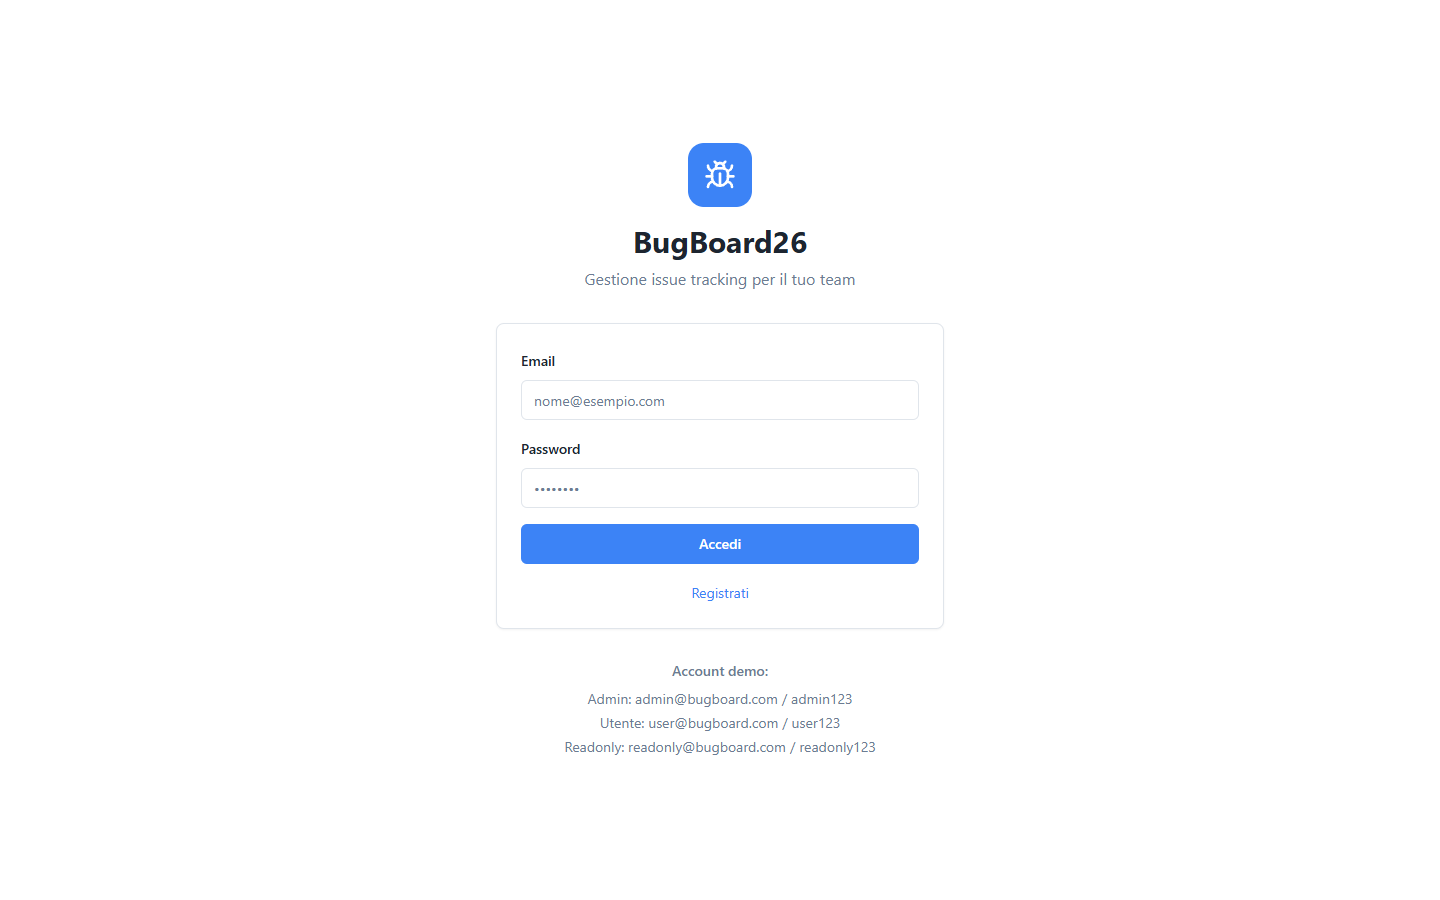
\includegraphics[width=0.85\textwidth]{immagini/mockup_01_login.png}
    \caption{Pagina di Login: form con email e password, pulsante di accesso}
    \label{fig:mockup_login}
\end{figure}

\begin{itemize}
    \item \textbf{Scopo}: autenticazione dell'utente al sistema
    \item \textbf{Elementi}: campo email, campo password, pulsante ``Accedi'', link alla pagina di registrazione
    \item \textbf{Comportamento}: in caso di credenziali errate viene mostrato un messaggio di errore inline; in caso di successo l'utente viene reindirizzato alla Dashboard
\end{itemize}

% ------- 2. REGISTRAZIONE -------
\subsubsection{Mock-up 2 --- Pagina di Registrazione}

\begin{figure}[H]
    \centering
    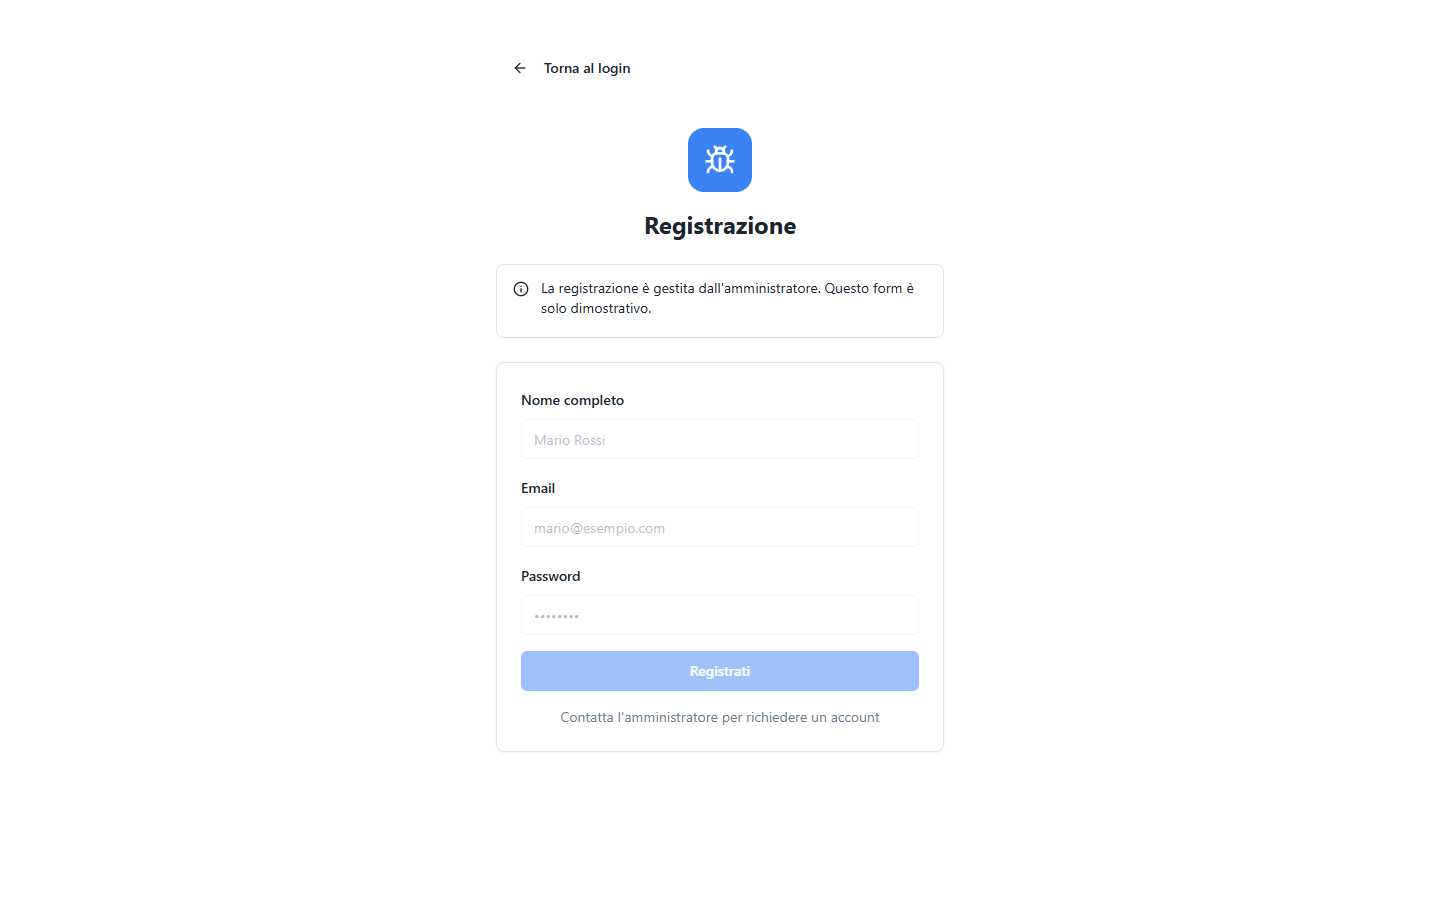
\includegraphics[width=0.85\textwidth]{immagini/mockup_02_register.png}
    \caption{Pagina di Registrazione: form con dati personali e creazione account}
    \label{fig:mockup_register}
\end{figure}

\begin{itemize}
    \item \textbf{Scopo}: creazione di un nuovo account utente
    \item \textbf{Elementi}: campi nome, email, password, conferma password; pulsante ``Registrati''
    \item \textbf{Validazione}: i campi vengono validati in tempo reale con messaggi di errore inline
\end{itemize}

% ------- 3. HOME -------
\subsubsection{Mock-up 3 --- Home / Dashboard}

\begin{figure}[H]
    \centering
    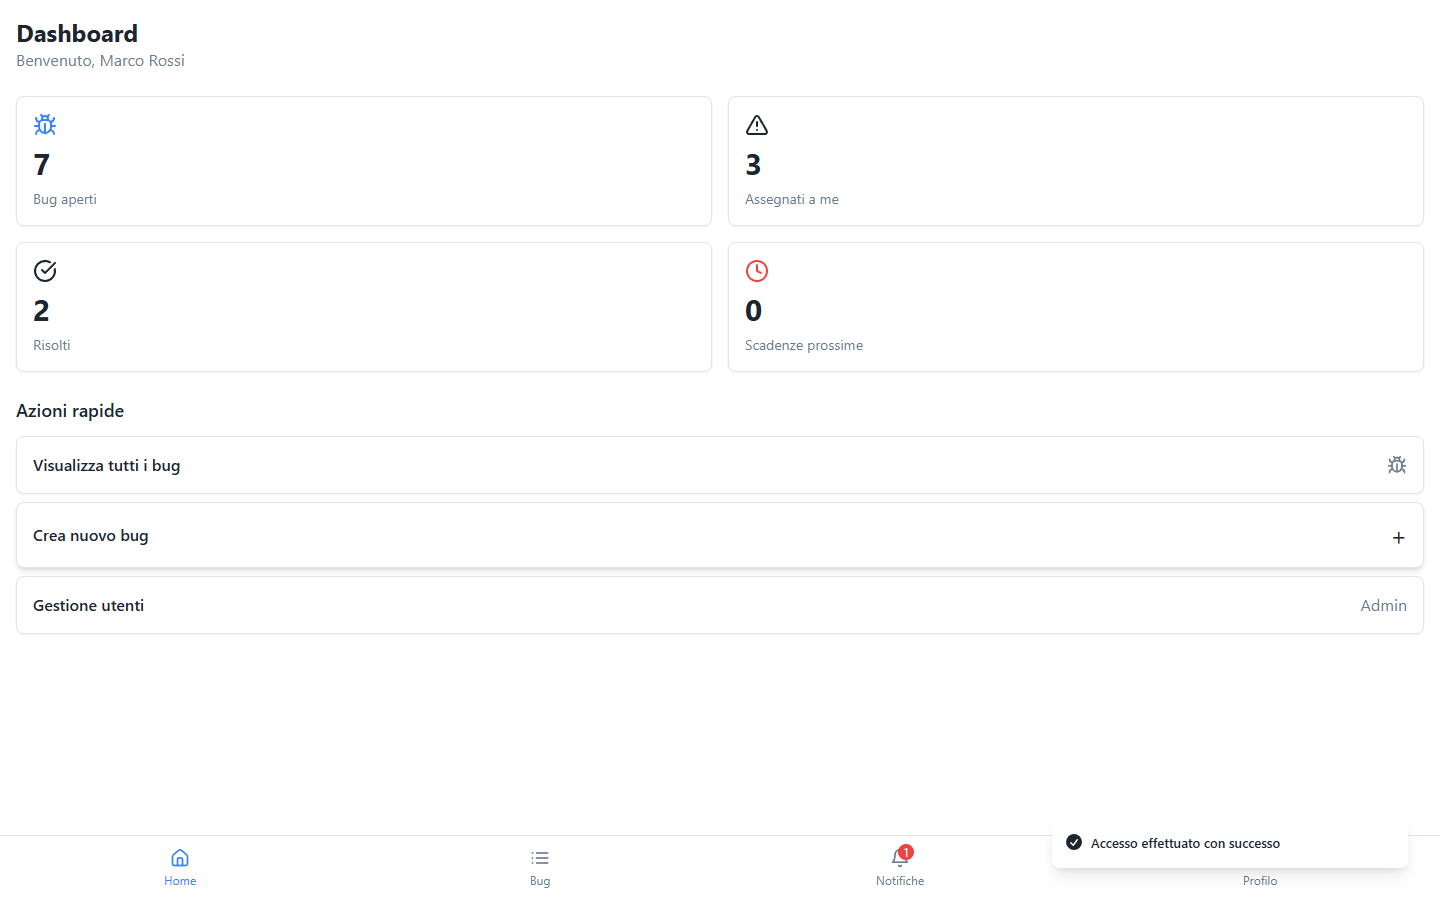
\includegraphics[width=0.85\textwidth]{immagini/mockup_03_home_dashboard.png}
    \caption{Home Dashboard: panoramica delle metriche principali e accessi rapidi}
    \label{fig:mockup_home}
\end{figure}

\begin{itemize}
    \item \textbf{Scopo}: fornire una panoramica immediata dello stato del sistema dopo il login
    \item \textbf{Elementi}: card metriche (bug aperti, assegnati a me, risolti, scadenze prossime), header con navigazione principale
    \item \textbf{Accessi rapidi}: da qui si può navigare alla lista bug, al form di creazione e ai report
\end{itemize}

% ------- 4. LISTA BUG -------
\subsubsection{Mock-up 4 --- Lista Bug con Filtri}

\begin{figure}[H]
    \centering
    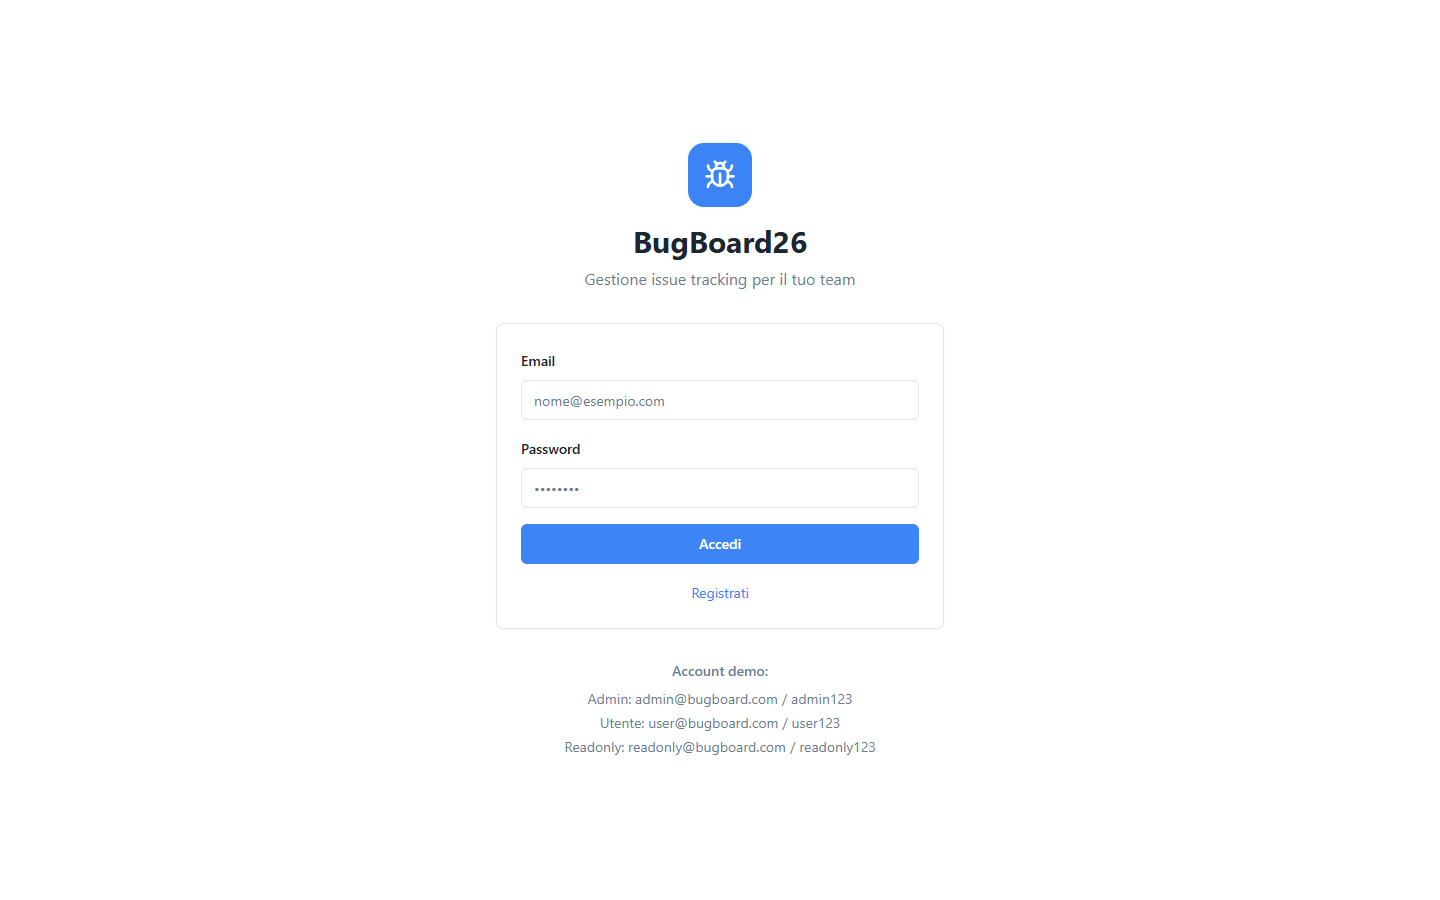
\includegraphics[width=0.85\textwidth]{immagini/mockup_04_lista_bug.png}
    \caption{Lista Bug: tabella con filtri per tipo, stato, priorità e ricerca testuale}
    \label{fig:mockup_lista_bug}
\end{figure}

\begin{itemize}
    \item \textbf{Scopo}: visualizzazione e filtraggio dell'elenco completo dei bug
    \item \textbf{Elementi}: barra filtri orizzontale (tipo, stato, priorità), campo ricerca full-text, tabella bug con badge colorati, paginazione
    \item \textbf{Interazione}: clic su una riga apre il dettaglio del bug; i filtri si applicano in tempo reale
\end{itemize}

% ------- 5. DETTAGLIO BUG -------
\subsubsection{Mock-up 5 --- Dettaglio Bug}

\begin{figure}[H]
    \centering
    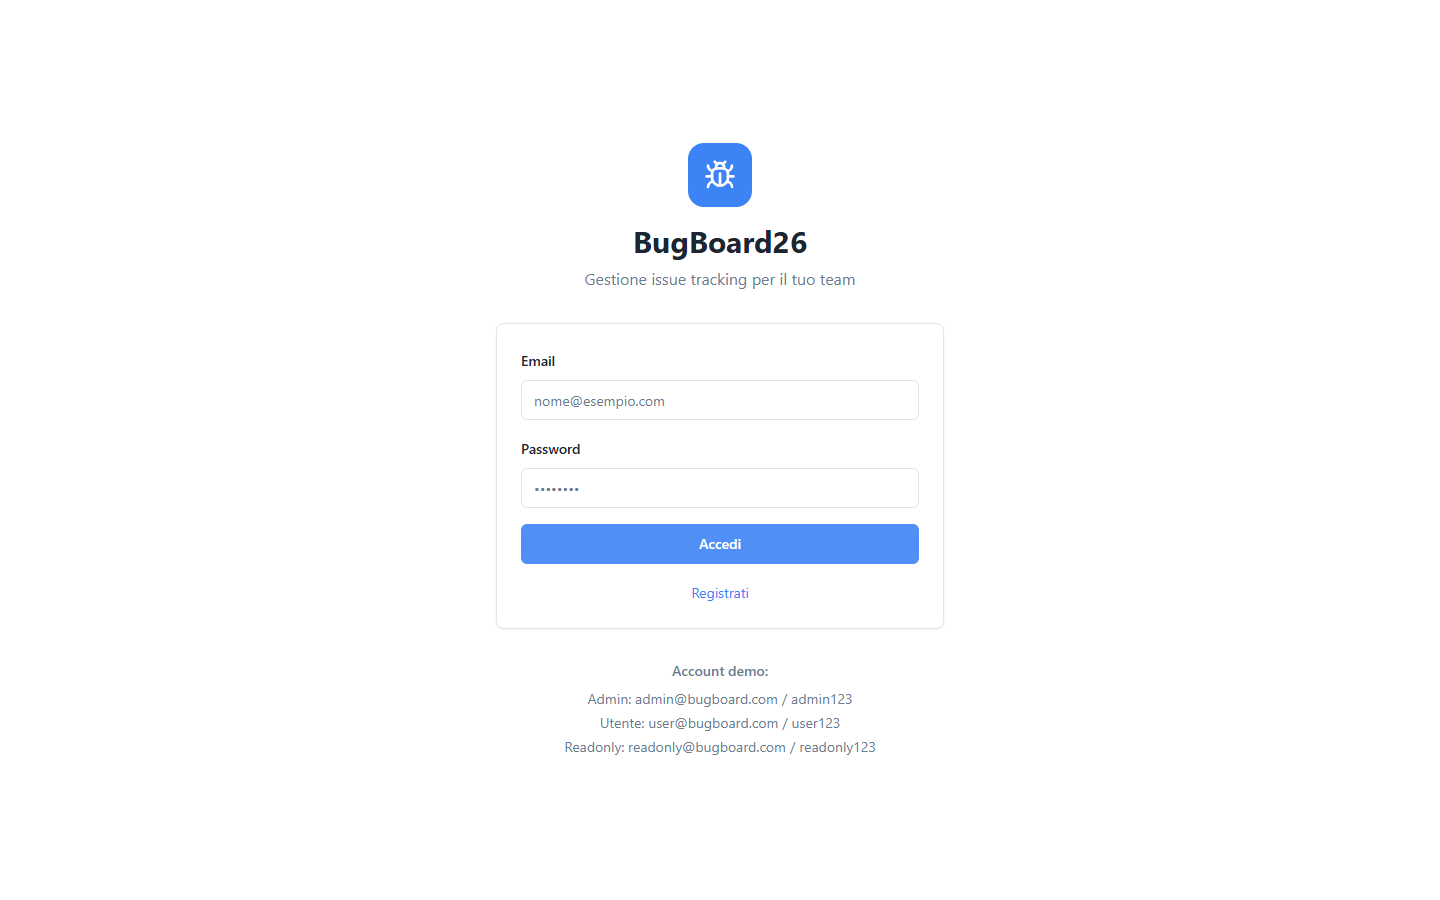
\includegraphics[width=0.85\textwidth]{immagini/mockup_05_dettaglio_bug.png}
    \caption{Dettaglio Bug: informazioni complete, commenti, storico modifiche e azioni disponibili}
    \label{fig:mockup_dettaglio_bug}
\end{figure}

\begin{itemize}
    \item \textbf{Scopo}: visualizzazione completa di un bug specifico e gestione delle azioni disponibili
    \item \textbf{Elementi}: header con titolo, stato e priorità; sezioni descrizione, commenti, allegati, storico; barra azioni laterale (modifica, assegna, risolvi, archivia, duplica)
    \item \textbf{Azioni visibili}: dipendono dal ruolo dell'utente (USER vede meno azioni rispetto ad Admin)
\end{itemize}

% ------- 6. FORM CREAZIONE BUG (UC01) -------
\subsubsection{Mock-up 6 --- Form Creazione/Modifica Bug \textbf{[UC01]}}

\begin{figure}[H]
    \centering
    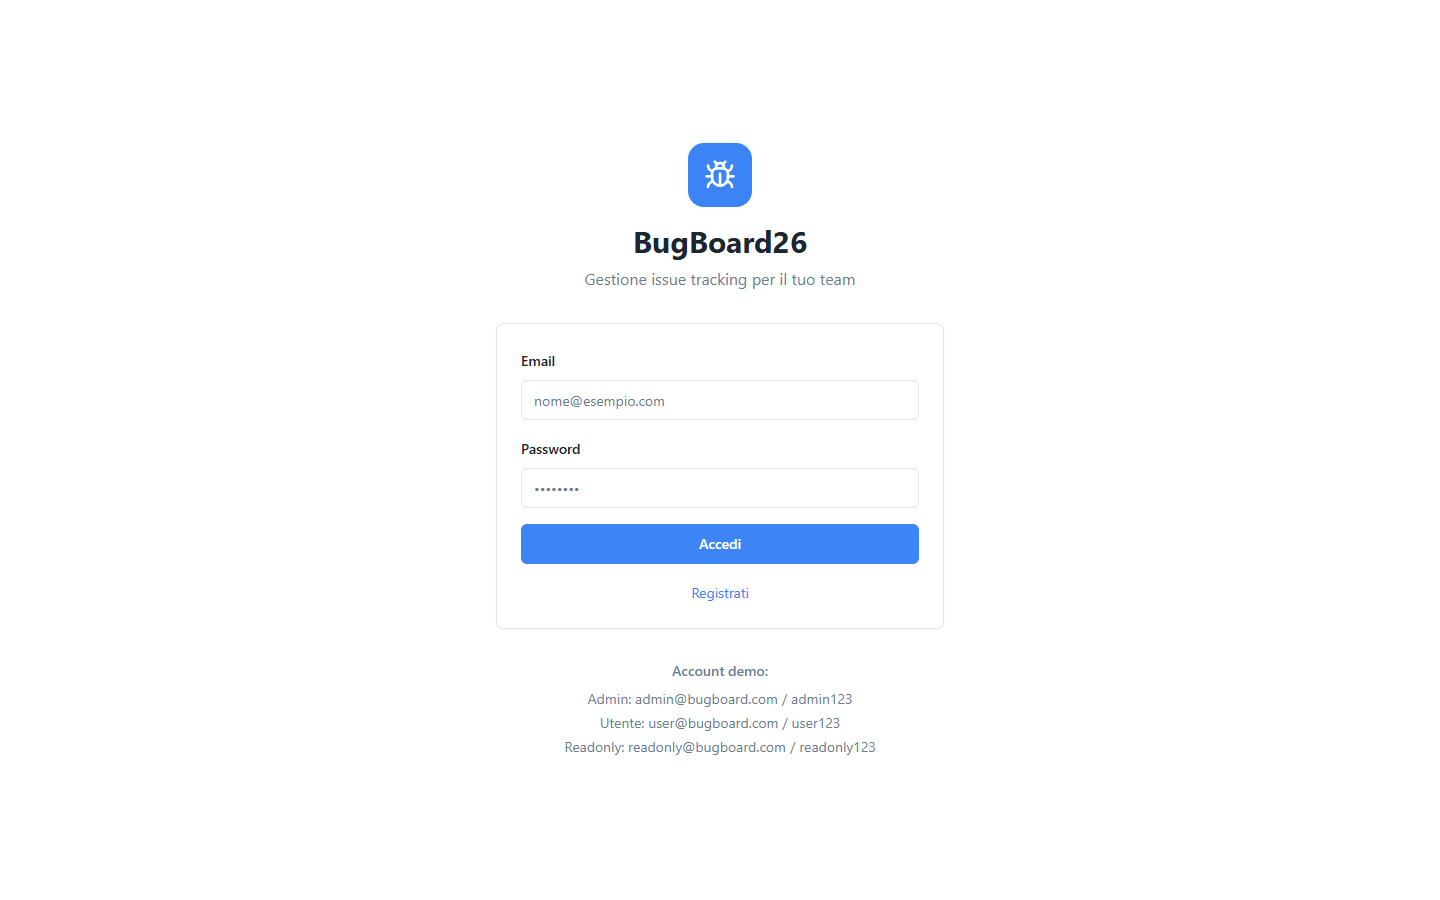
\includegraphics[width=0.85\textwidth]{immagini/mockup_06_form_creazione_bug.png}
    \caption{Form Creazione Bug (UC01): campi titolo, tipo, priorità, descrizione, label, allegati}
    \label{fig:mockup_form_bug}
\end{figure}

\begin{itemize}
    \item \textbf{Caso d'uso}: UC01 --- Creazione nuovo bug
    \item \textbf{Elementi}: campo titolo, selettori tipo e priorità, area di testo descrizione, selezione label multipla, upload allegati immagine, selezione assegnatario opzionale, pulsante ``Salva''
    \item \textbf{Validazione}: i campi obbligatori (titolo, tipo, priorità) sono evidenziati se lasciati vuoti; il formato e la dimensione degli allegati sono verificati prima dell'invio
\end{itemize}

% ------- 7. ASSEGNAZIONE BUG (UC02) -------
\subsubsection{Mock-up 7 --- Assegnazione Bug \textbf{[UC02]}}

\begin{figure}[H]
    \centering
    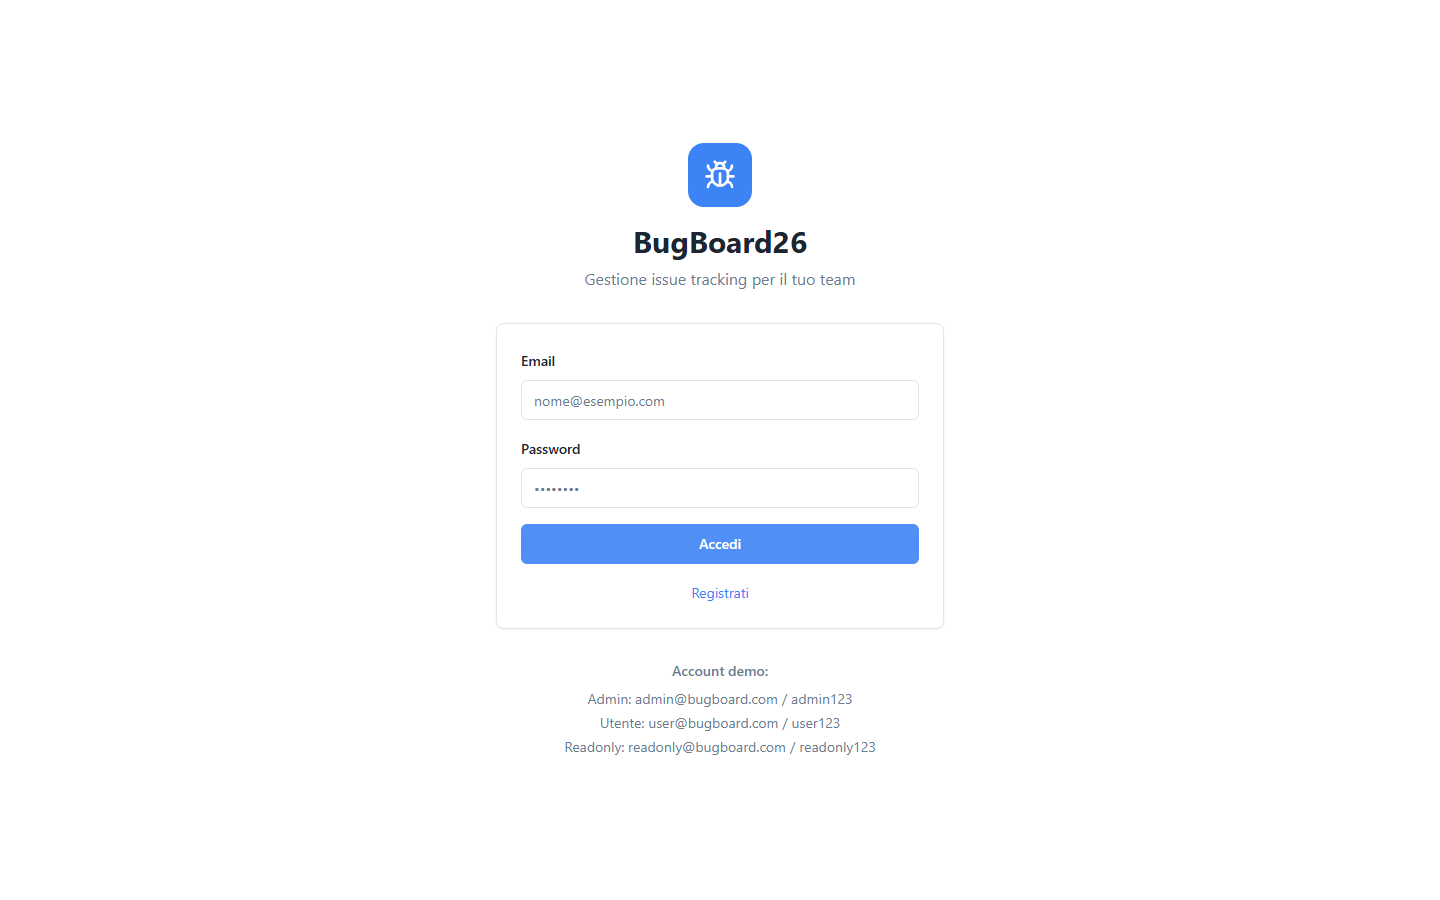
\includegraphics[width=0.85\textwidth]{immagini/mockup_07_assegnazione_bug.png}
    \caption{Assegnazione Bug (UC02): selezione dell'utente a cui assegnare il bug}
    \label{fig:mockup_assegnazione}
\end{figure}

\begin{itemize}
    \item \textbf{Caso d'uso}: UC02 --- Assegnazione bug a un utente (solo Admin)
    \item \textbf{Elementi}: select per la scelta dell'utente assegnatario, pulsante conferma
    \item \textbf{Accesso}: questa schermata è accessibile solo agli utenti con ruolo Admin; un USER viene reindirizzato alla Dashboard
\end{itemize}

% ------- 8. NOTIFICHE -------
\subsubsection{Mock-up 8 --- Notifiche}

\begin{figure}[H]
    \centering
    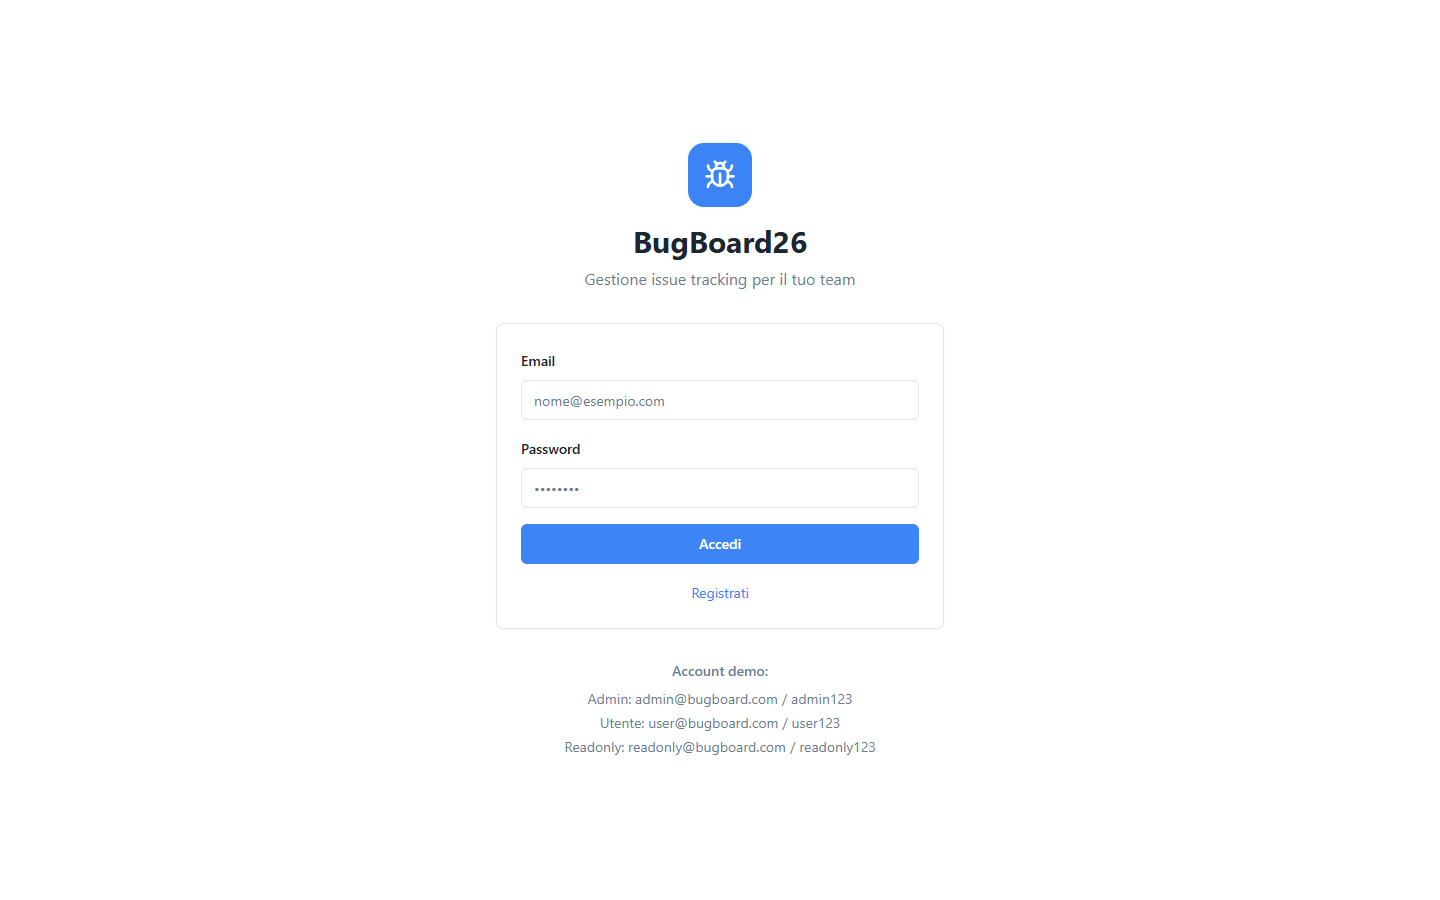
\includegraphics[width=0.85\textwidth]{immagini/mockup_08_notifiche.png}
    \caption{Centro Notifiche: lista degli aggiornamenti sui bug seguiti dall'utente}
    \label{fig:mockup_notifiche}
\end{figure}

\begin{itemize}
    \item \textbf{Scopo}: mostrare all'utente gli aggiornamenti recenti sui bug che lo riguardano (assegnazioni, cambi stato, nuovi commenti)
    \item \textbf{Elementi}: lista notifiche con timestamp, tipo evento e link al bug correlato; indicatore notifiche non lette
\end{itemize}

% ------- 9. PROFILO -------
\subsubsection{Mock-up 9 --- Profilo Utente}

\begin{figure}[H]
    \centering
    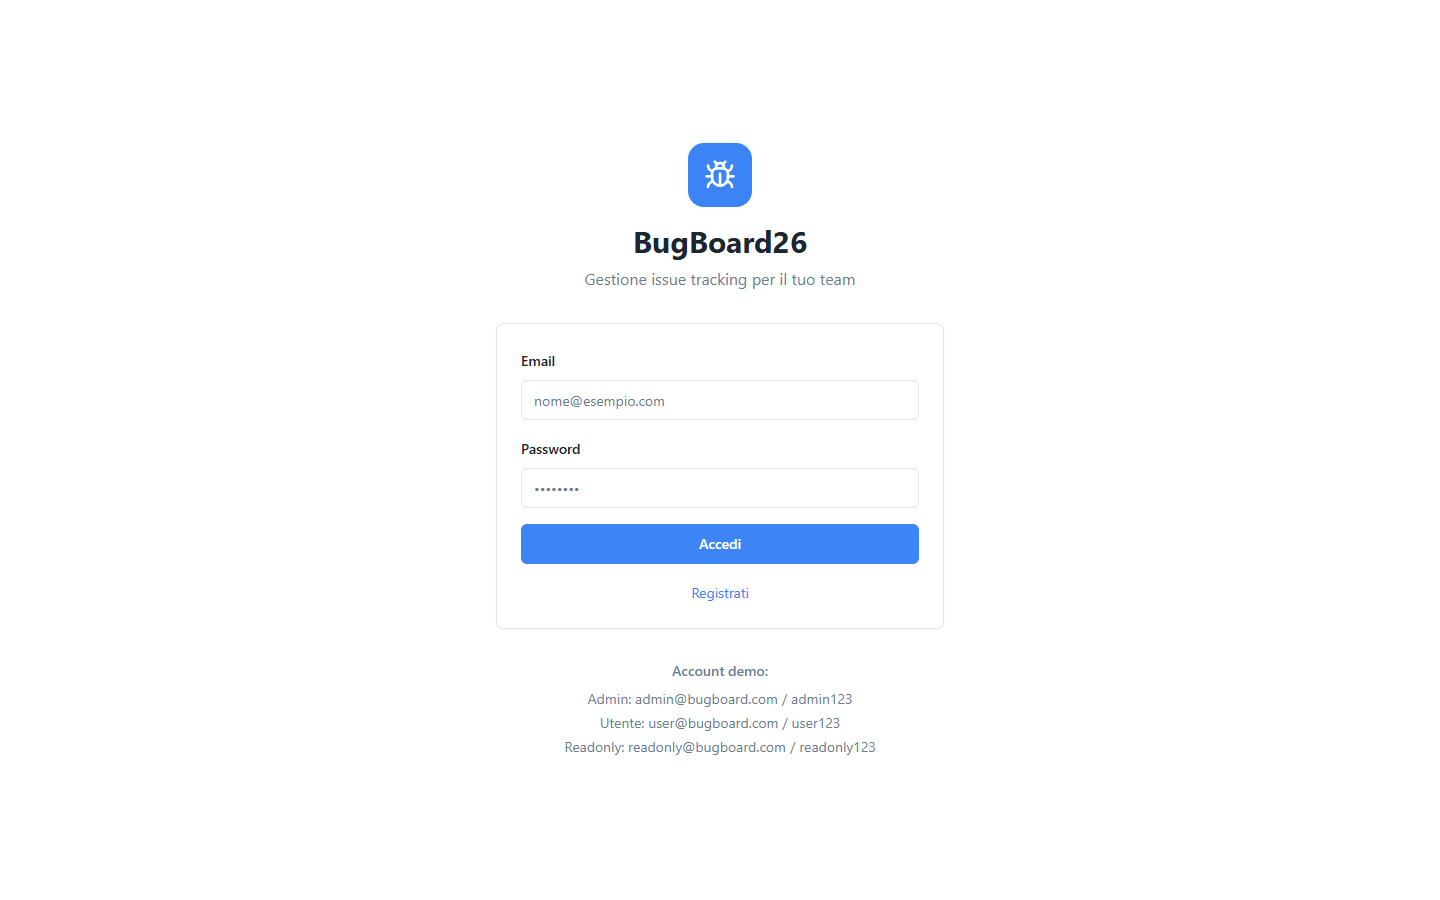
\includegraphics[width=0.85\textwidth]{immagini/mockup_09_profilo.png}
    \caption{Profilo Utente: gestione informazioni personali e cambio password}
    \label{fig:mockup_profilo}
\end{figure}

\begin{itemize}
    \item \textbf{Scopo}: consentire all'utente di visualizzare e modificare le proprie informazioni e la password
    \item \textbf{Elementi}: nome, email, ruolo (in sola lettura), form cambio password con validazione
\end{itemize}

% ------- 10. REPORT MENSILE (UC04) -------
\subsubsection{Mock-up 10 --- Report Mensile \textbf{[UC04]}}

\begin{figure}[H]
    \centering
    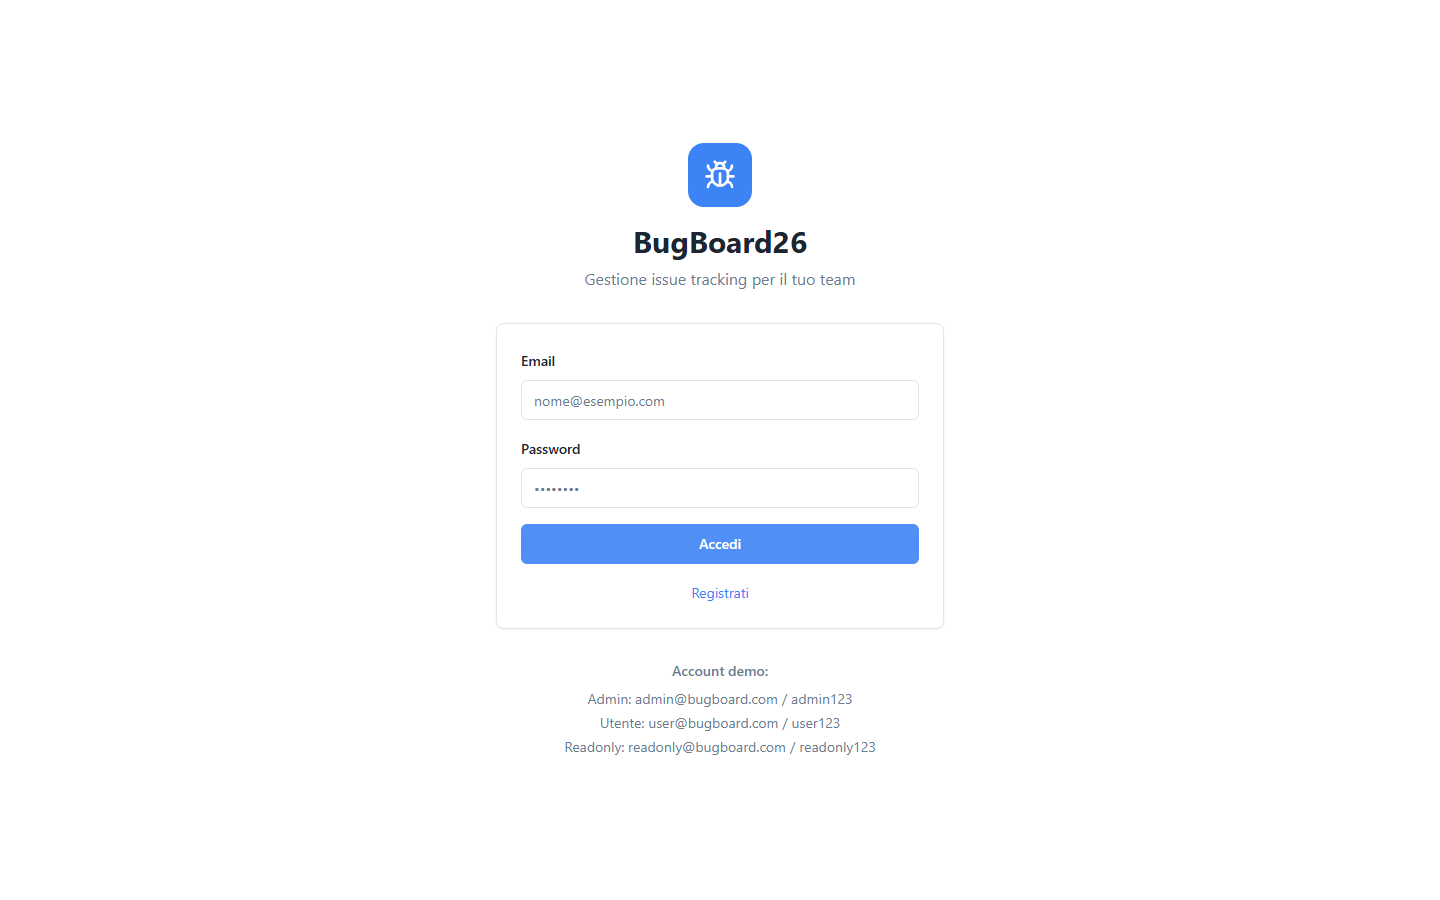
\includegraphics[width=0.85\textwidth]{immagini/mockup_10_report_mensile.png}
    \caption{Report Mensile Admin (UC04): statistiche, grafici e pulsante di export Excel}
    \label{fig:mockup_report}
\end{figure}

\begin{itemize}
    \item \textbf{Caso d'uso}: UC04 --- Generazione report mensile (solo Admin)
    \item \textbf{Elementi}: selettore mese/anno, grafici (distribuzione stato, priorità, trend temporale), tabella riassuntiva metriche, pulsante ``Esporta Excel''
    \item \textbf{Accesso}: solo Admin; gli altri utenti vengono reindirizzati alla Dashboard
\end{itemize}

% ------- 11. GESTIONE UTENTI ADMIN -------
\subsubsection{Mock-up 11 --- Gestione Utenti (Admin)}

\begin{figure}[H]
    \centering
    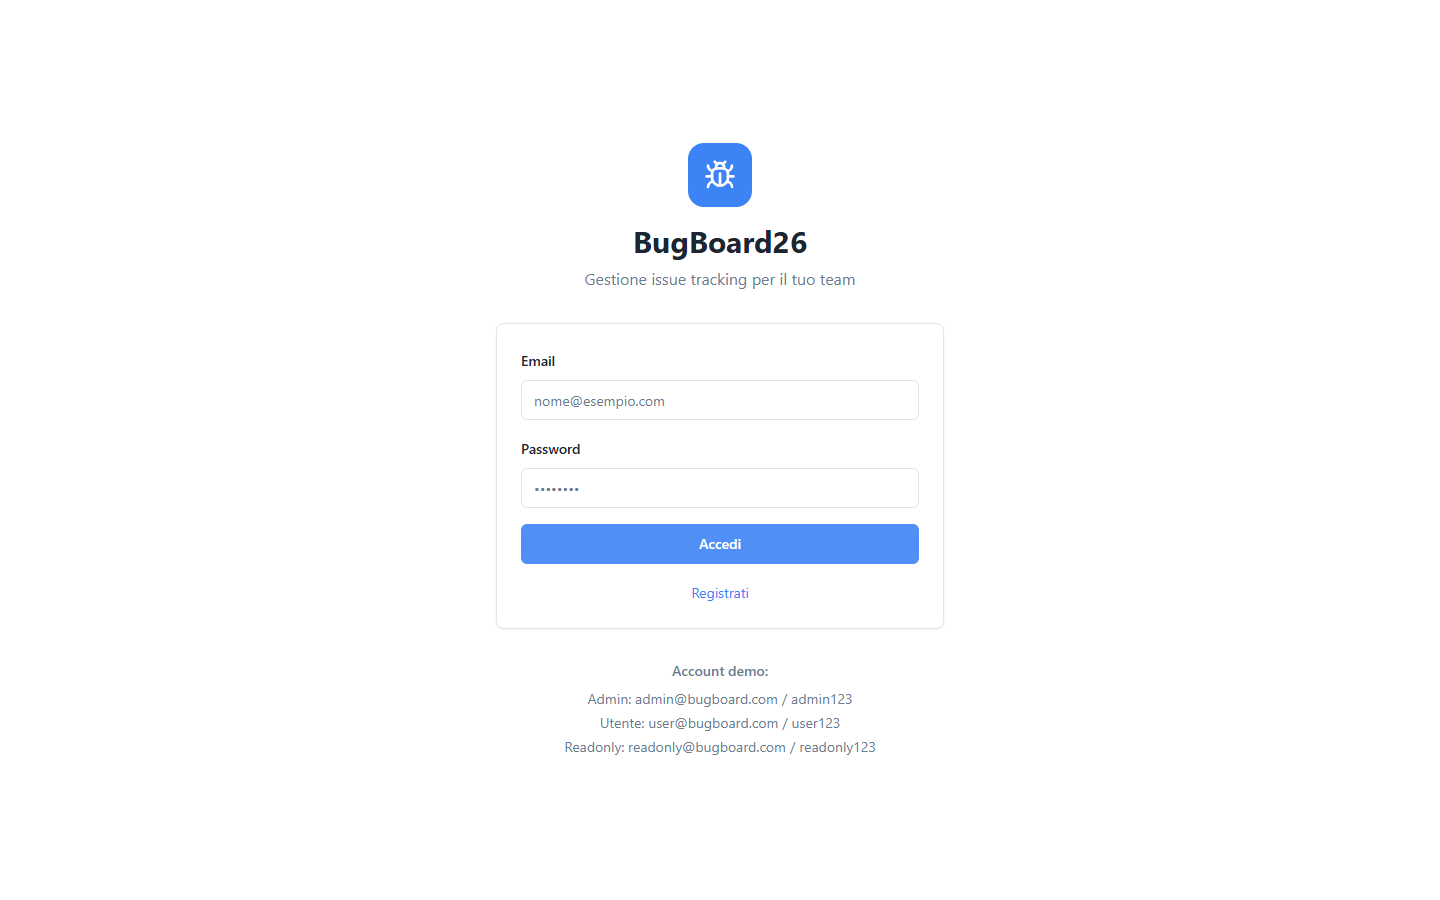
\includegraphics[width=0.85\textwidth]{immagini/mockup_11_admin_utenti.png}
    \caption{Gestione Utenti Admin: lista utenti con ruoli, stato e azioni di modifica}
    \label{fig:mockup_admin_utenti}
\end{figure}

\begin{itemize}
    \item \textbf{Scopo}: permettere all'Admin di gestire gli account del sistema (visualizzazione ruoli, disabilitazione utenti)
    \item \textbf{Elementi}: tabella utenti con email, nome, ruolo e stato; azioni per modifica ruolo e disabilitazione account
\end{itemize}

% ------- 12. ARCHIVIO -------
\subsubsection{Mock-up 12 --- Archivio Bug}

\begin{figure}[H]
    \centering
    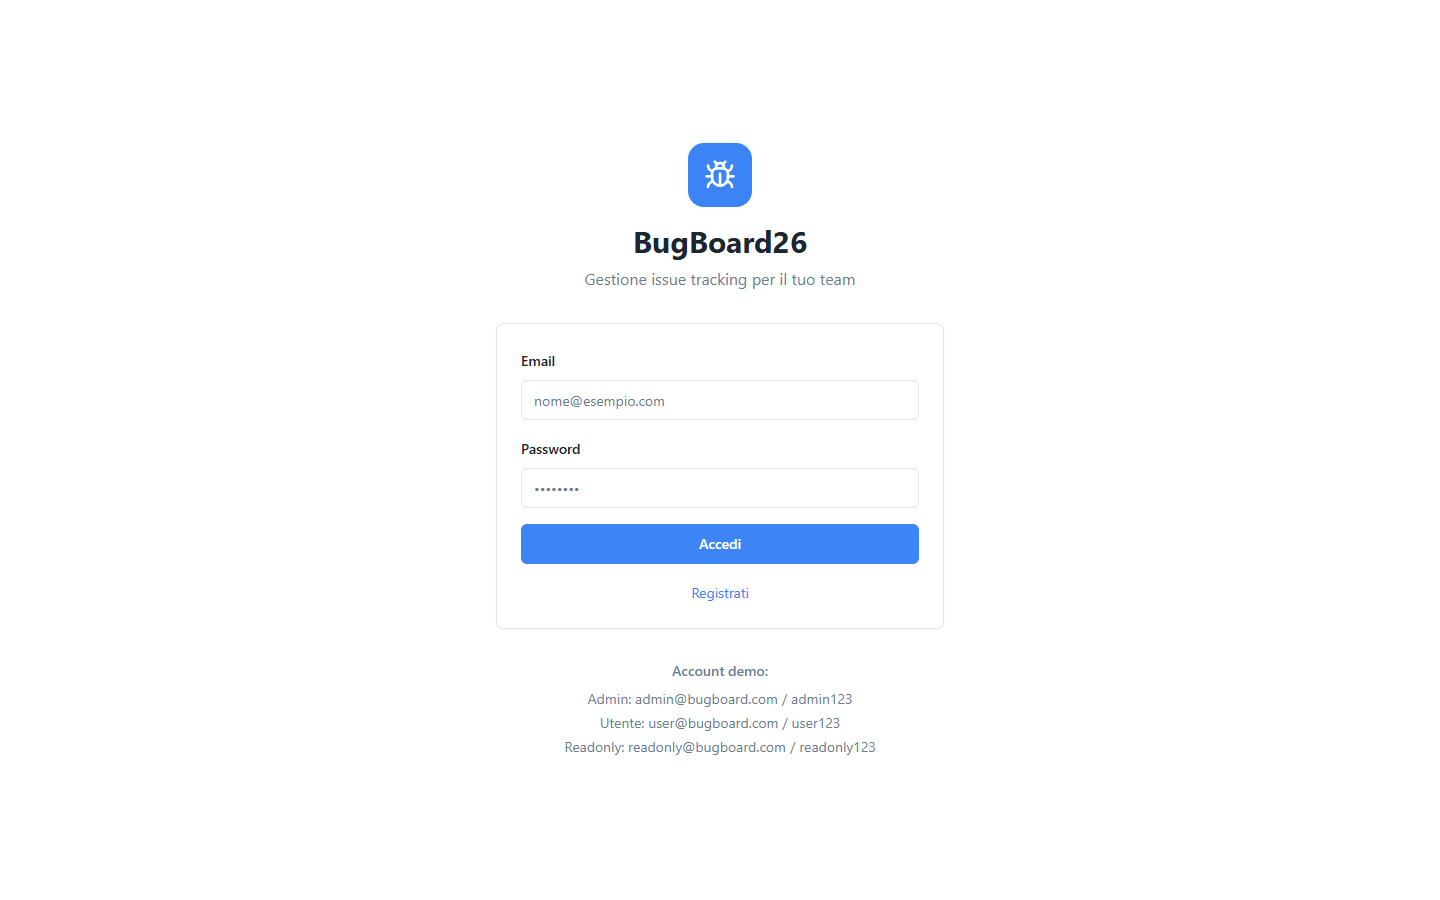
\includegraphics[width=0.85\textwidth]{immagini/mockup_12_archivio.png}
    \caption{Archivio Bug: lista dei bug archiviati con possibilità di consultazione}
    \label{fig:mockup_archivio}
\end{figure}

\begin{itemize}
    \item \textbf{Scopo}: visualizzare i bug archiviati per storico e consultazione senza influire sulla lista attiva
    \item \textbf{Elementi}: tabella bug in stato \textit{Archived} con filtri e ricerca; solo Admin può archiviare/ripristinare bug
\end{itemize}

% ------- 13. EXPORT -------
\subsubsection{Mock-up 13 --- Export Dati}

\begin{figure}[H]
    \centering
    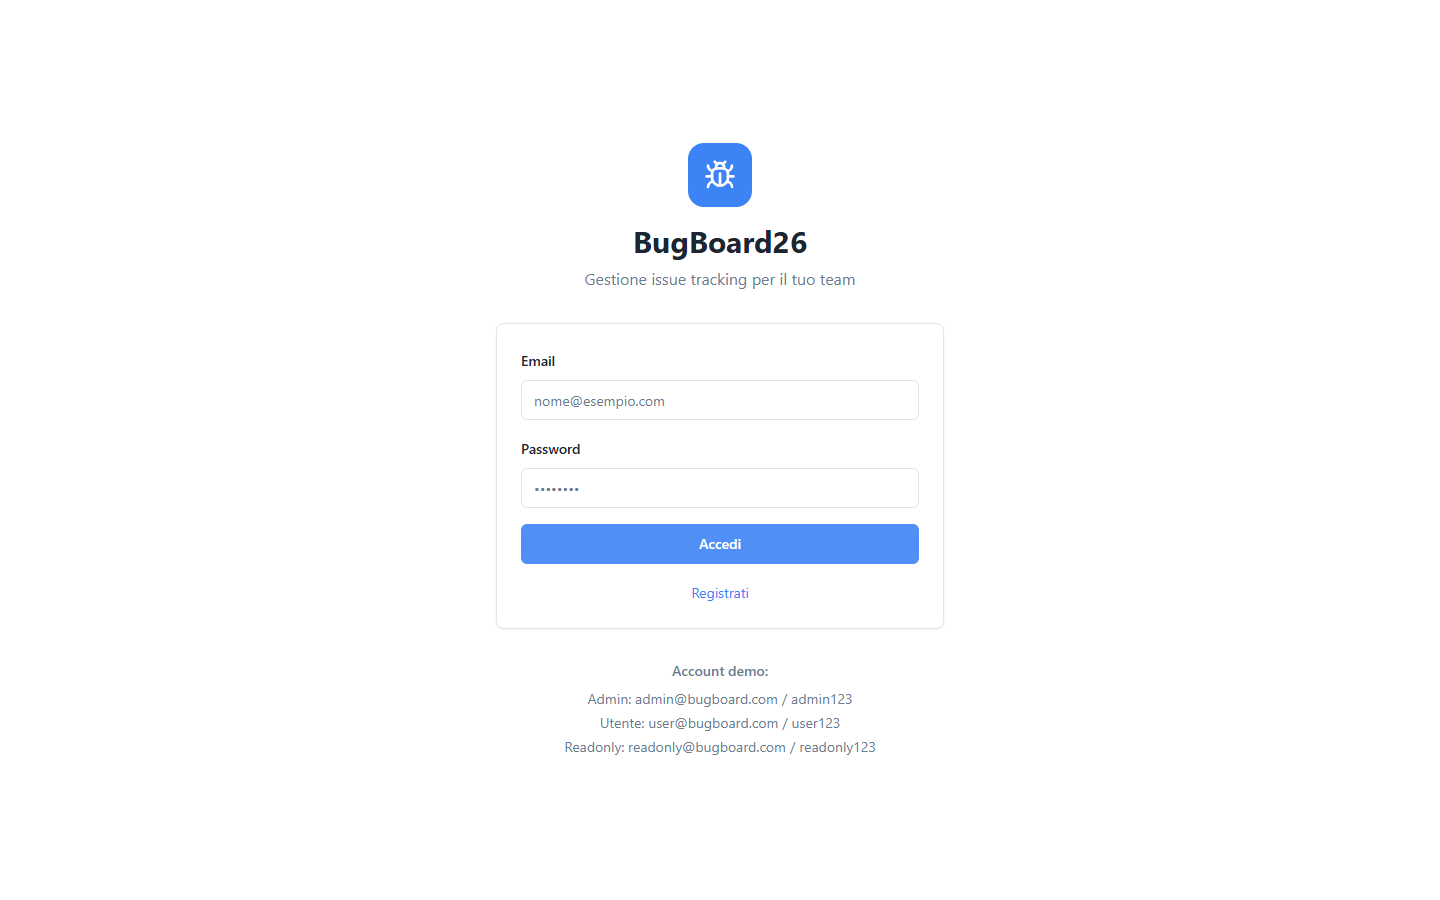
\includegraphics[width=0.85\textwidth]{immagini/mockup_13_export.png}
    \caption{Export Dati: download dell'elenco bug in formato CSV o Excel}
    \label{fig:mockup_export}
\end{figure}

\begin{itemize}
    \item \textbf{Scopo}: consentire l'esportazione dei dati per analisi esterne
    \item \textbf{Elementi}: pulsanti ``Scarica CSV'' e ``Scarica Excel''; i file vengono generati dal backend e scaricati direttamente
\end{itemize}

% ------------------------------------------------------------
\subsection{Osservazioni emerse dalla prototipazione}

La realizzazione del prototipo funzionante ha permesso di identificare alcune scelte migliorative rispetto all'analisi iniziale:

\begin{itemize}
    \item \textbf{Chiarezza dei ruoli}: è stato necessario rendere esplicito nel UI quali azioni sono riservate all'Admin (assegnazione, report, archiviazione, gestione utenti), aggiungendo reindirizzamenti automatici per utenti non autorizzati
    \item \textbf{Filtri immediati}: la lista bug con filtri in tempo reale si è rivelata la funzionalità più usata nelle sessioni di test, confermando la scelta di renderla la pagina principale
    \item \textbf{Badge colorati}: l'uso di badge cromatici per stato, priorità e tipo ha migliorato significativamente la leggibilità della lista bug senza aprire il dettaglio
    \item \textbf{Navigazione mobile}: il menu hamburger con le stesse voci del desktop ha garantito piena parità funzionale su dispositivi mobili
\end{itemize}

% ============================================================

\section{Prototipazione visuale attraverso Mock-up}

La prototipazione visuale di BugBoard26 è stata realizzata direttamente come applicazione React funzionante, con dati simulati (\textit{mock data}). Le schermate qui mostrate sono catture reali del prototipo interattivo, e non semplici bozzetti grafici. Questo approccio ha permesso di validare il flusso utente in modo concreto fin dalla fase di analisi.

% ------------------------------------------------------------
\subsection{Scelte Progettuali}

\subsubsection{Layout e Navigazione}
\begin{itemize}
    \item \textbf{Header fisso}: barra superiore con logo, link alle sezioni principali (Dashboard, Bug, Report, Admin) e menu utente con avatar, email e pulsante logout
    \item \textbf{Navigazione mobile}: menu a comparsa (hamburger) con le stesse voci, ottimizzato per touch
    \item \textbf{Layout responsive}: design \textit{mobile-first} realizzato con Tailwind CSS; le griglie si adattano automaticamente a qualsiasi larghezza schermo
\end{itemize}

\subsubsection{Palette Colori e Badge}
\begin{itemize}
    \item \textbf{Priorità}: \textit{Critical} (rosso), \textit{High} (arancione), \textit{Medium} (giallo), \textit{Low} (verde)
    \item \textbf{Stato}: \textit{Todo} (grigio chiaro), \textit{In Progress} (blu), \textit{Resolved} (verde), \textit{Archived} (grigio scuro)
    \item \textbf{Tipo}: \textit{Bug} (rosso), \textit{Feature} (viola), \textit{Enhancement} (azzurro)
    \item \textbf{Azioni primarie}: blu (\texttt{\#007BFF}); superfici neutre: grigi Tailwind
\end{itemize}

\subsubsection{Componenti UI riutilizzati}
Tutti i componenti sono basati su \textbf{Radix UI} e \textbf{shadcn/ui}: Button, Card, Select, Dialog, Badge, Table, Toast, DropdownMenu. Questo garantisce coerenza visiva e accessibilità WCAG 2.1 out-of-the-box.

% ------------------------------------------------------------
\subsection{Mock-up delle interfacce utente}

Di seguito sono illustrate le schermate principali del prototipo, raggruppate per funzionalità. Le schermate contrassegnate con \textbf{[UC0X]} corrispondono direttamente ai casi d'uso formalizzati nella sezione precedente.

% ------- 1. LOGIN -------
\subsubsection{Mock-up 1 --- Pagina di Login}

\begin{figure}[H]
    \centering
    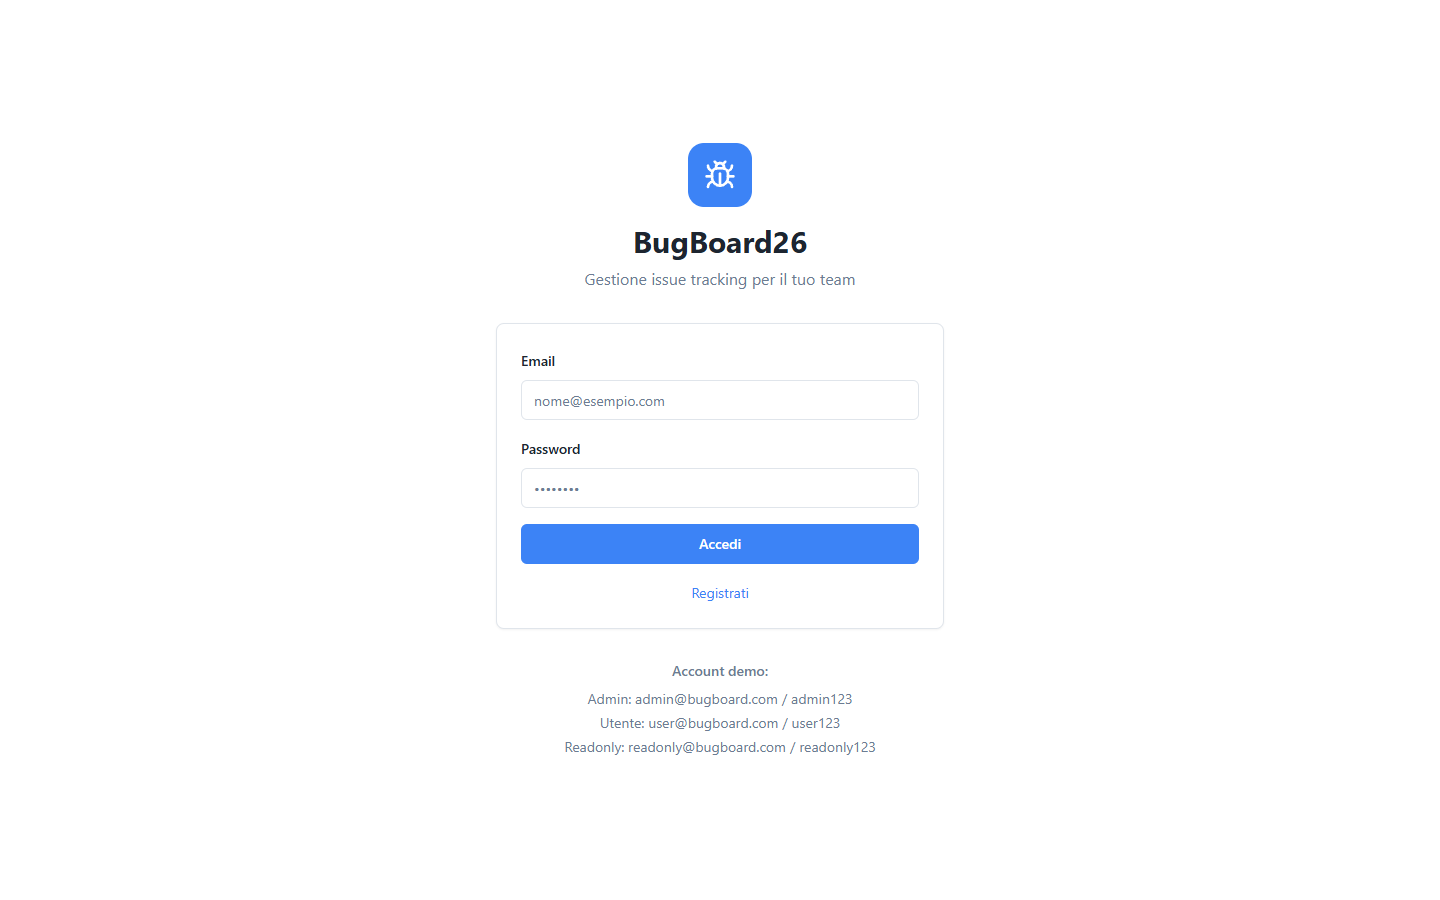
\includegraphics[width=0.85\textwidth]{immagini/mockup_01_login.png}
    \caption{Pagina di Login: form con email e password, pulsante di accesso}
    \label{fig:mockup_login}
\end{figure}

\begin{itemize}
    \item \textbf{Scopo}: autenticazione dell'utente al sistema
    \item \textbf{Elementi}: campo email, campo password, pulsante ``Accedi'', link alla pagina di registrazione
    \item \textbf{Comportamento}: in caso di credenziali errate viene mostrato un messaggio di errore inline; in caso di successo l'utente viene reindirizzato alla Dashboard
\end{itemize}

% ------- 2. REGISTRAZIONE -------
\subsubsection{Mock-up 2 --- Pagina di Registrazione}

\begin{figure}[H]
    \centering
    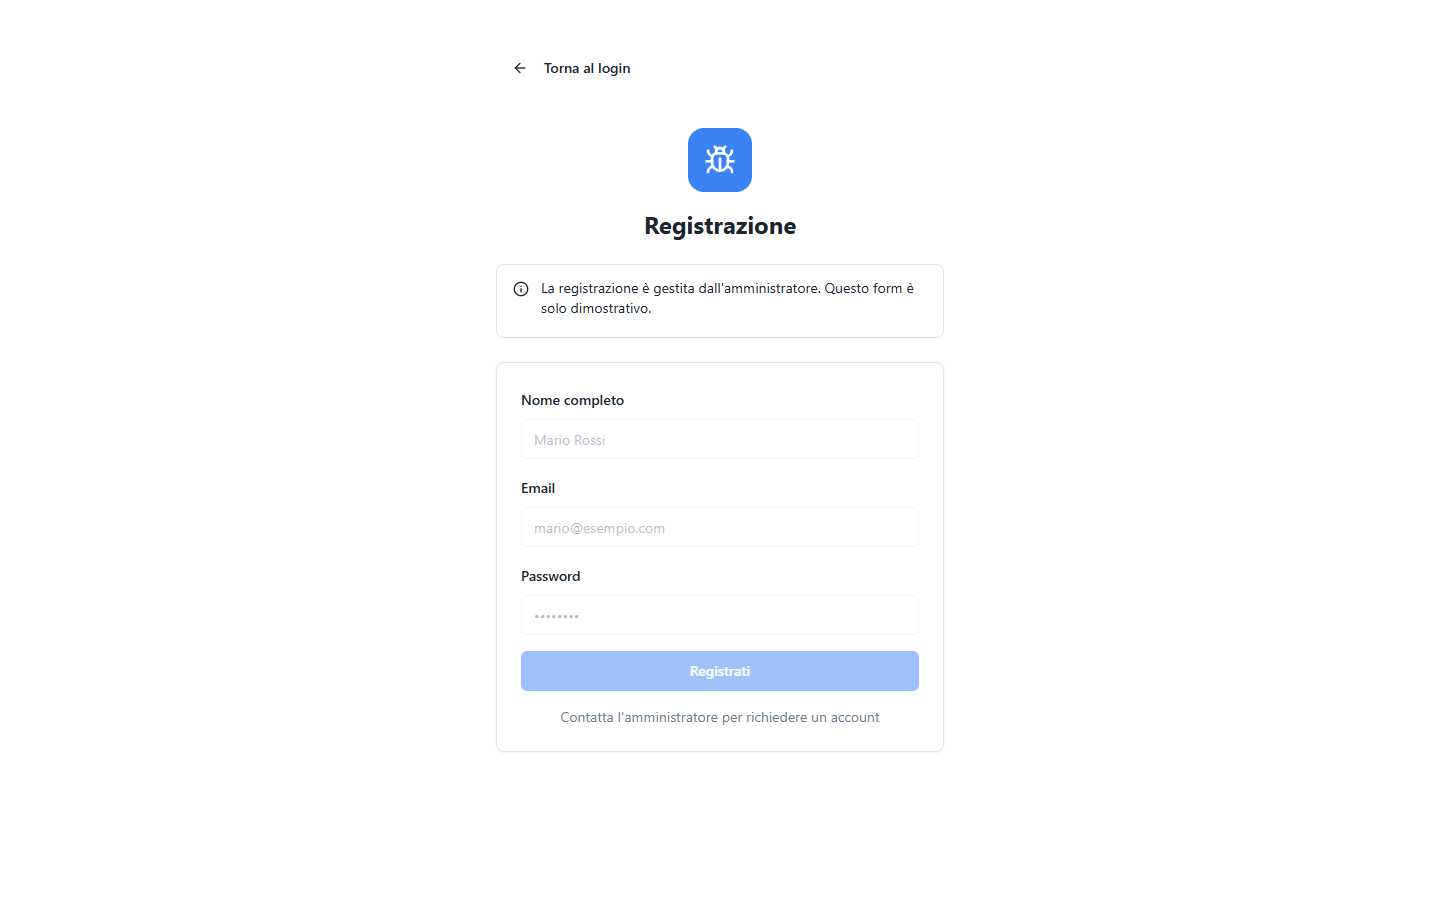
\includegraphics[width=0.85\textwidth]{immagini/mockup_02_register.png}
    \caption{Pagina di Registrazione: form con dati personali e creazione account}
    \label{fig:mockup_register}
\end{figure}

\begin{itemize}
    \item \textbf{Scopo}: creazione di un nuovo account utente
    \item \textbf{Elementi}: campi nome, email, password, conferma password; pulsante ``Registrati''
    \item \textbf{Validazione}: i campi vengono validati in tempo reale con messaggi di errore inline
\end{itemize}

% ------- 3. HOME -------
\subsubsection{Mock-up 3 --- Home / Dashboard}

\begin{figure}[H]
    \centering
    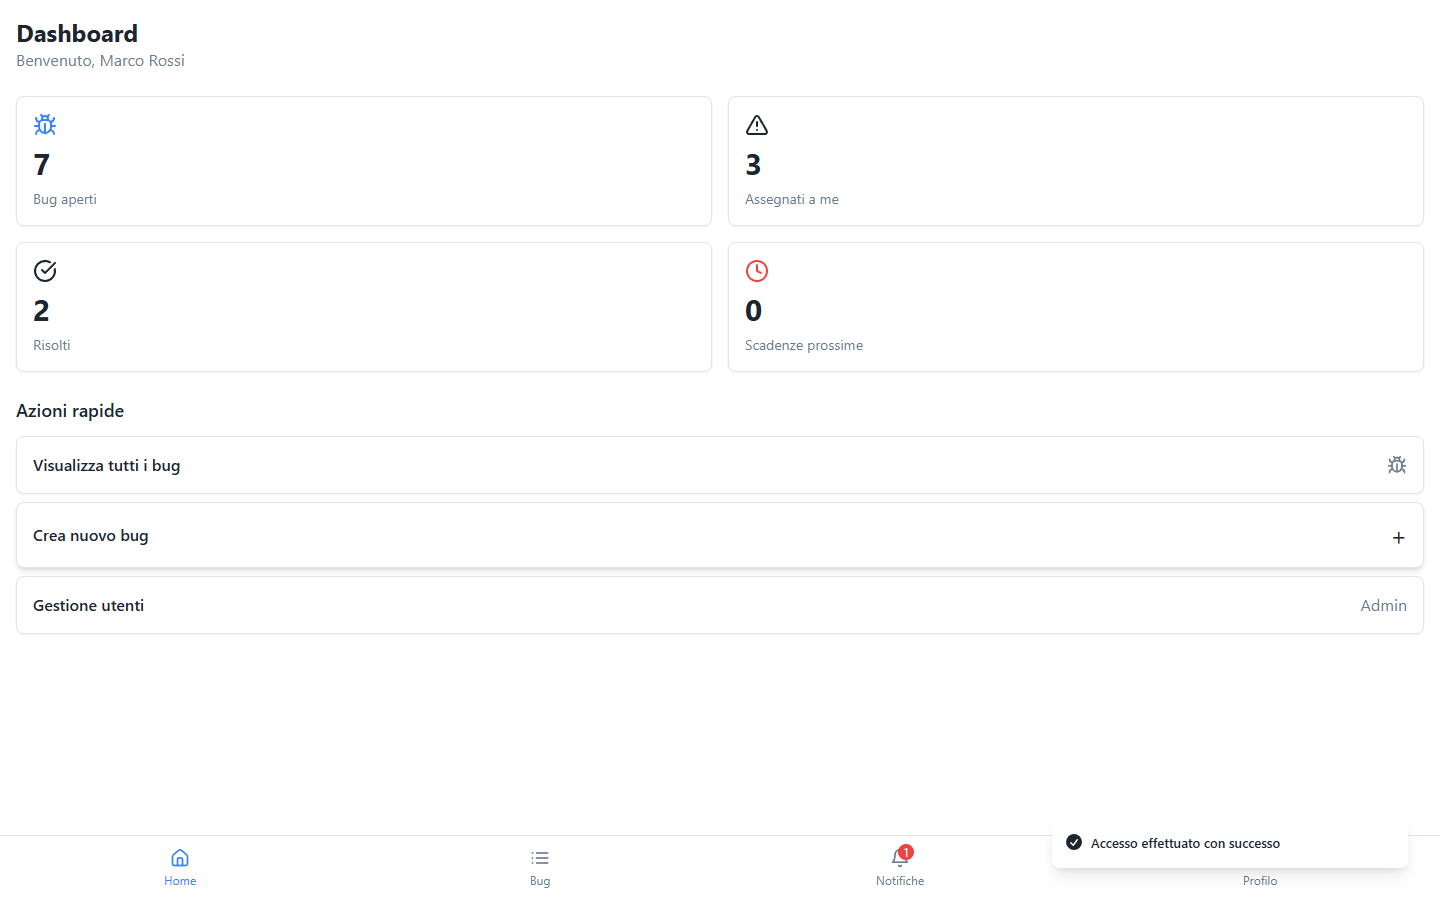
\includegraphics[width=0.85\textwidth]{immagini/mockup_03_home_dashboard.png}
    \caption{Home Dashboard: panoramica delle metriche principali e accessi rapidi}
    \label{fig:mockup_home}
\end{figure}

\begin{itemize}
    \item \textbf{Scopo}: fornire una panoramica immediata dello stato del sistema dopo il login
    \item \textbf{Elementi}: card metriche (bug aperti, assegnati a me, risolti, scadenze prossime), header con navigazione principale
    \item \textbf{Accessi rapidi}: da qui si può navigare alla lista bug, al form di creazione e ai report
\end{itemize}

% ------- 4. LISTA BUG -------
\subsubsection{Mock-up 4 --- Lista Bug con Filtri}

\begin{figure}[H]
    \centering
    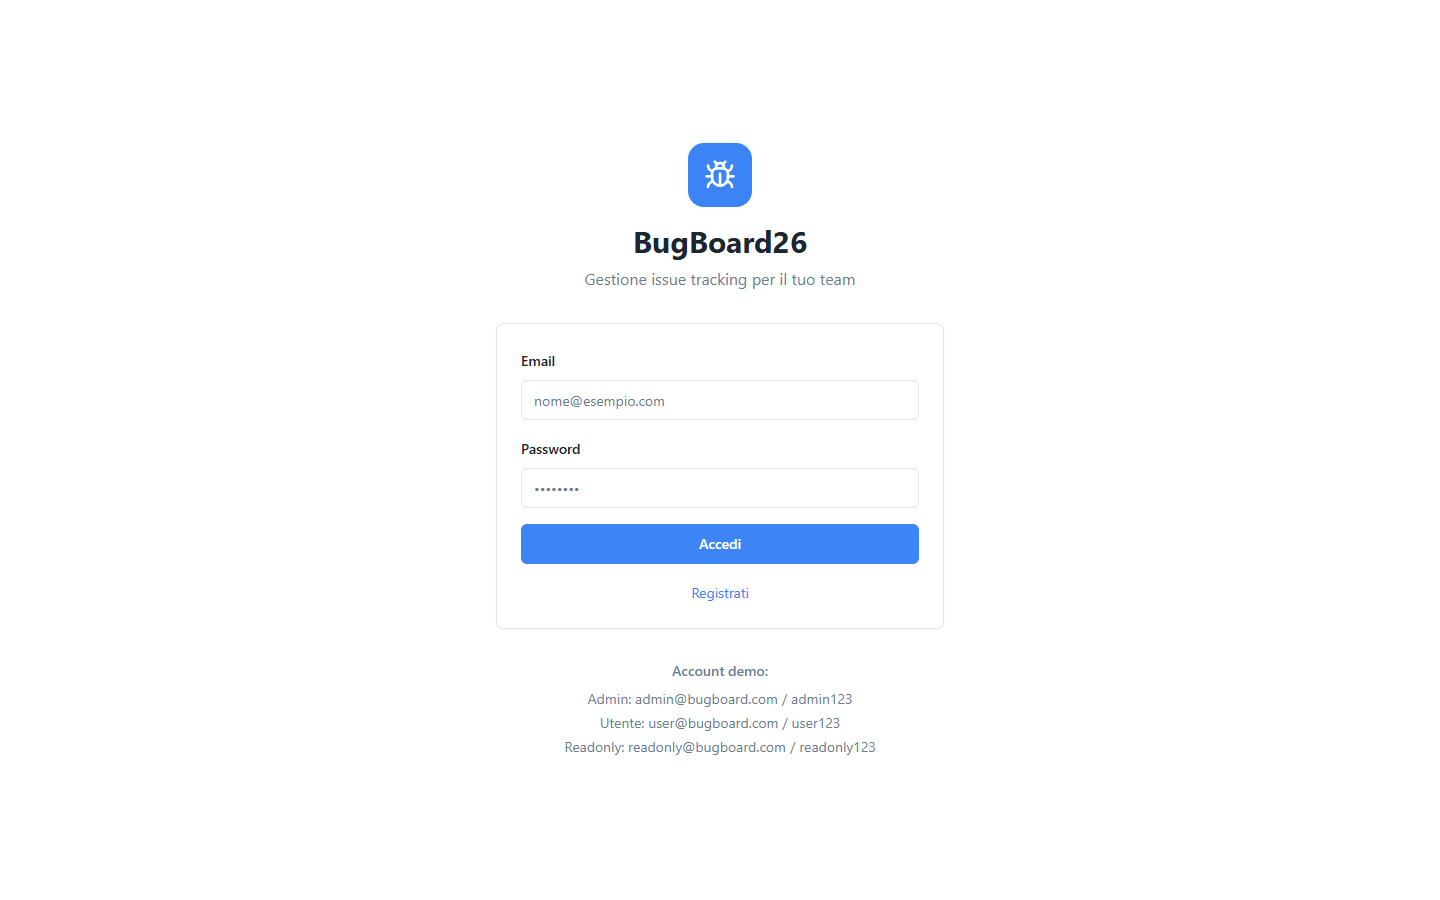
\includegraphics[width=0.85\textwidth]{immagini/mockup_04_lista_bug.png}
    \caption{Lista Bug: tabella con filtri per tipo, stato, priorità e ricerca testuale}
    \label{fig:mockup_lista_bug}
\end{figure}

\begin{itemize}
    \item \textbf{Scopo}: visualizzazione e filtraggio dell'elenco completo dei bug
    \item \textbf{Elementi}: barra filtri orizzontale (tipo, stato, priorità), campo ricerca full-text, tabella bug con badge colorati, paginazione
    \item \textbf{Interazione}: clic su una riga apre il dettaglio del bug; i filtri si applicano in tempo reale
\end{itemize}

% ------- 5. DETTAGLIO BUG -------
\subsubsection{Mock-up 5 --- Dettaglio Bug}

\begin{figure}[H]
    \centering
    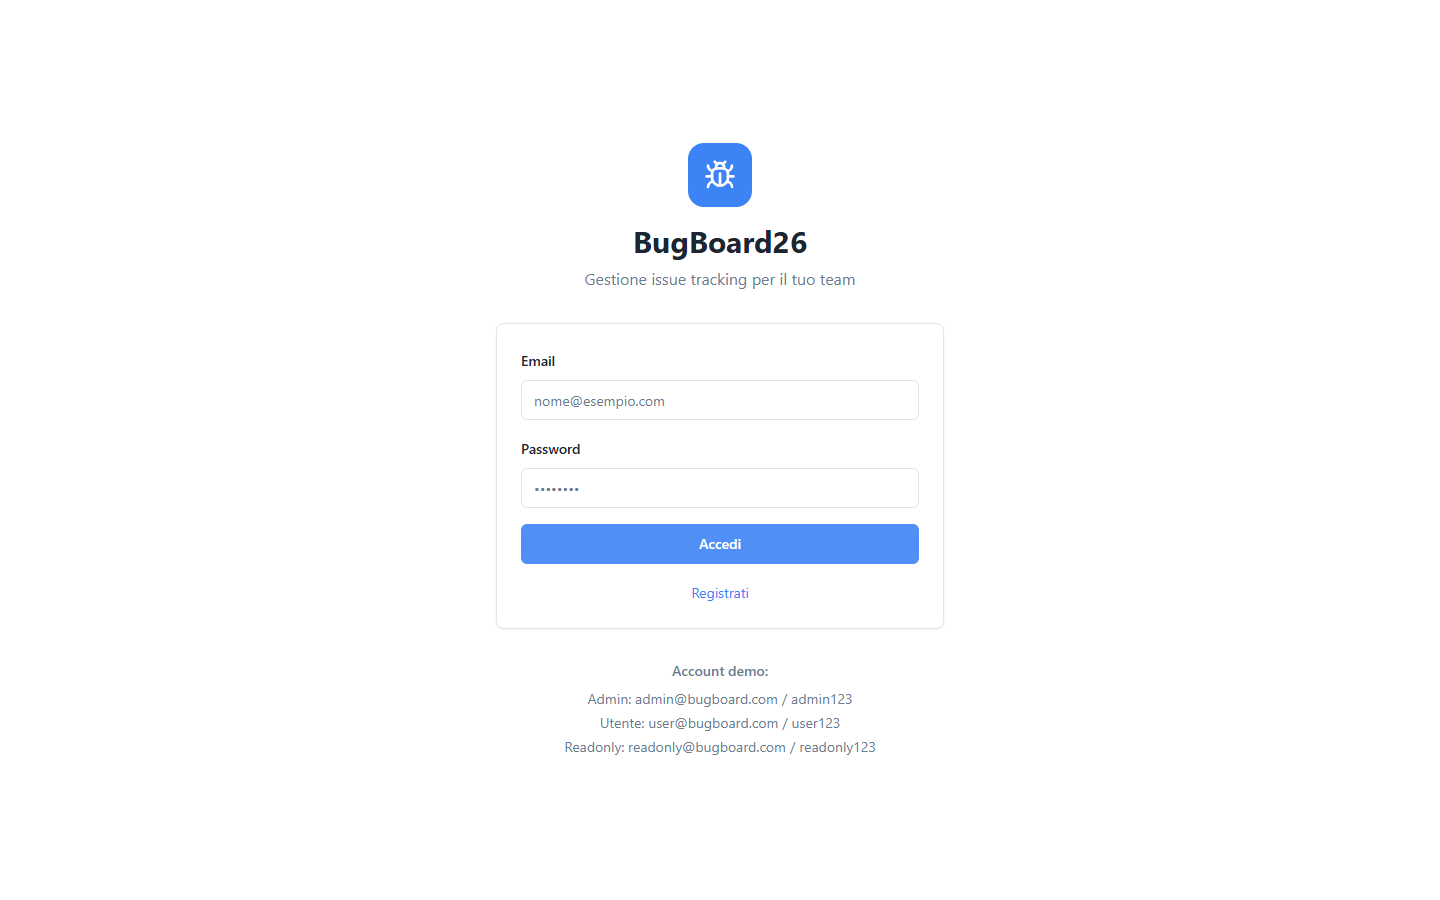
\includegraphics[width=0.85\textwidth]{immagini/mockup_05_dettaglio_bug.png}
    \caption{Dettaglio Bug: informazioni complete, commenti, storico modifiche e azioni disponibili}
    \label{fig:mockup_dettaglio_bug}
\end{figure}

\begin{itemize}
    \item \textbf{Scopo}: visualizzazione completa di un bug specifico e gestione delle azioni disponibili
    \item \textbf{Elementi}: header con titolo, stato e priorità; sezioni descrizione, commenti, allegati, storico; barra azioni laterale (modifica, assegna, risolvi, archivia, duplica)
    \item \textbf{Azioni visibili}: dipendono dal ruolo dell'utente (USER vede meno azioni rispetto ad Admin)
\end{itemize}

% ------- 6. FORM CREAZIONE BUG (UC01) -------
\subsubsection{Mock-up 6 --- Form Creazione/Modifica Bug \textbf{[UC01]}}

\begin{figure}[H]
    \centering
    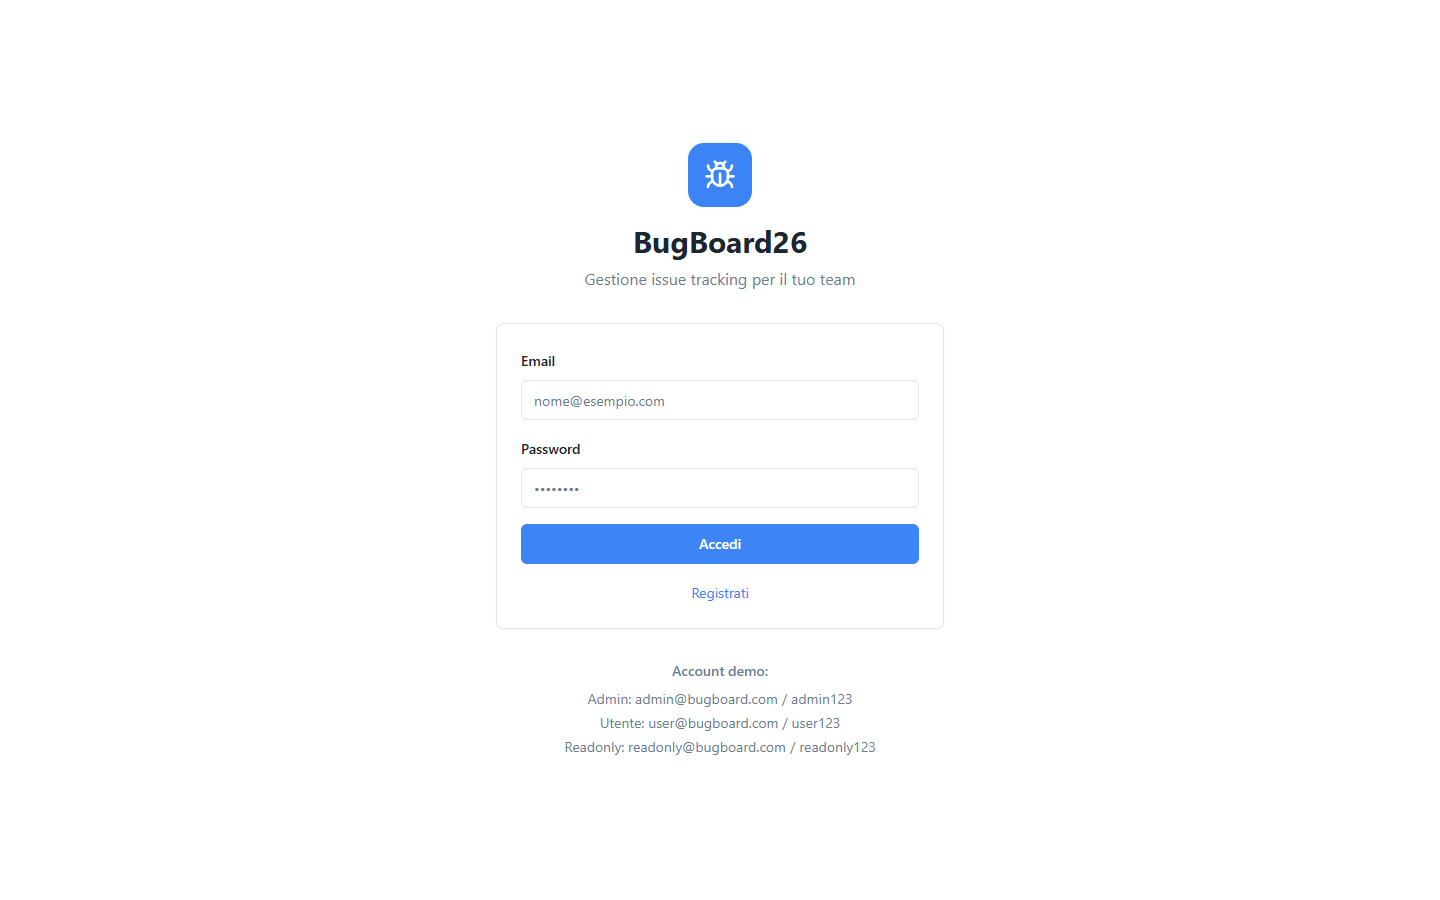
\includegraphics[width=0.85\textwidth]{immagini/mockup_06_form_creazione_bug.png}
    \caption{Form Creazione Bug (UC01): campi titolo, tipo, priorità, descrizione, label, allegati}
    \label{fig:mockup_form_bug}
\end{figure}

\begin{itemize}
    \item \textbf{Caso d'uso}: UC01 --- Creazione nuovo bug
    \item \textbf{Elementi}: campo titolo, selettori tipo e priorità, area di testo descrizione, selezione label multipla, upload allegati immagine, selezione assegnatario opzionale, pulsante ``Salva''
    \item \textbf{Validazione}: i campi obbligatori (titolo, tipo, priorità) sono evidenziati se lasciati vuoti; il formato e la dimensione degli allegati sono verificati prima dell'invio
\end{itemize}

% ------- 7. ASSEGNAZIONE BUG (UC02) -------
\subsubsection{Mock-up 7 --- Assegnazione Bug \textbf{[UC02]}}

\begin{figure}[H]
    \centering
    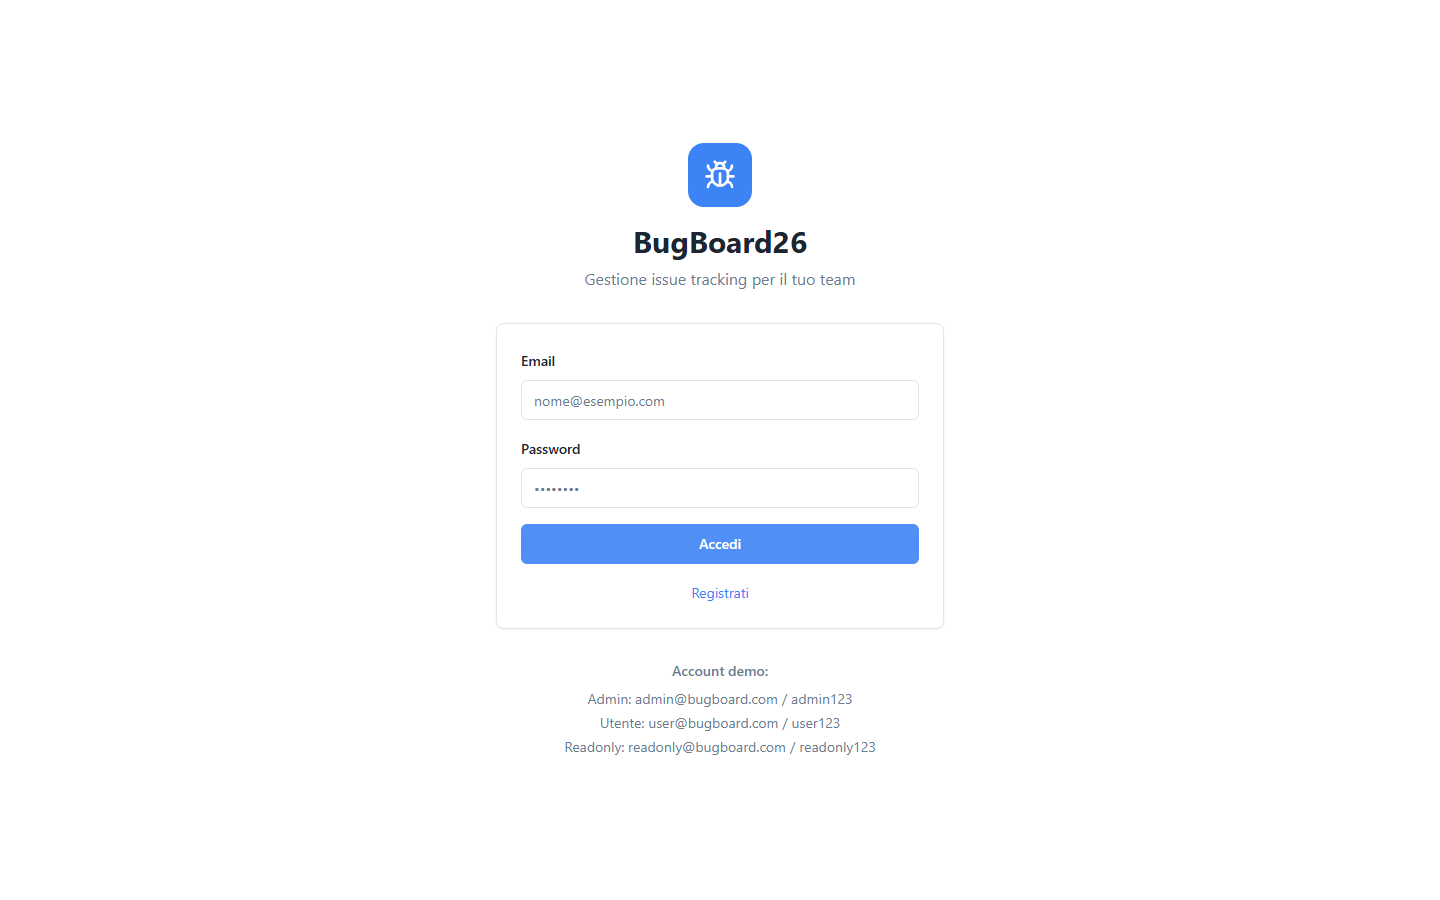
\includegraphics[width=0.85\textwidth]{immagini/mockup_07_assegnazione_bug.png}
    \caption{Assegnazione Bug (UC02): selezione dell'utente a cui assegnare il bug}
    \label{fig:mockup_assegnazione}
\end{figure}

\begin{itemize}
    \item \textbf{Caso d'uso}: UC02 --- Assegnazione bug a un utente (solo Admin)
    \item \textbf{Elementi}: select per la scelta dell'utente assegnatario, pulsante conferma
    \item \textbf{Accesso}: questa schermata è accessibile solo agli utenti con ruolo Admin; un USER viene reindirizzato alla Dashboard
\end{itemize}

% ------- 8. NOTIFICHE -------
\subsubsection{Mock-up 8 --- Notifiche}

\begin{figure}[H]
    \centering
    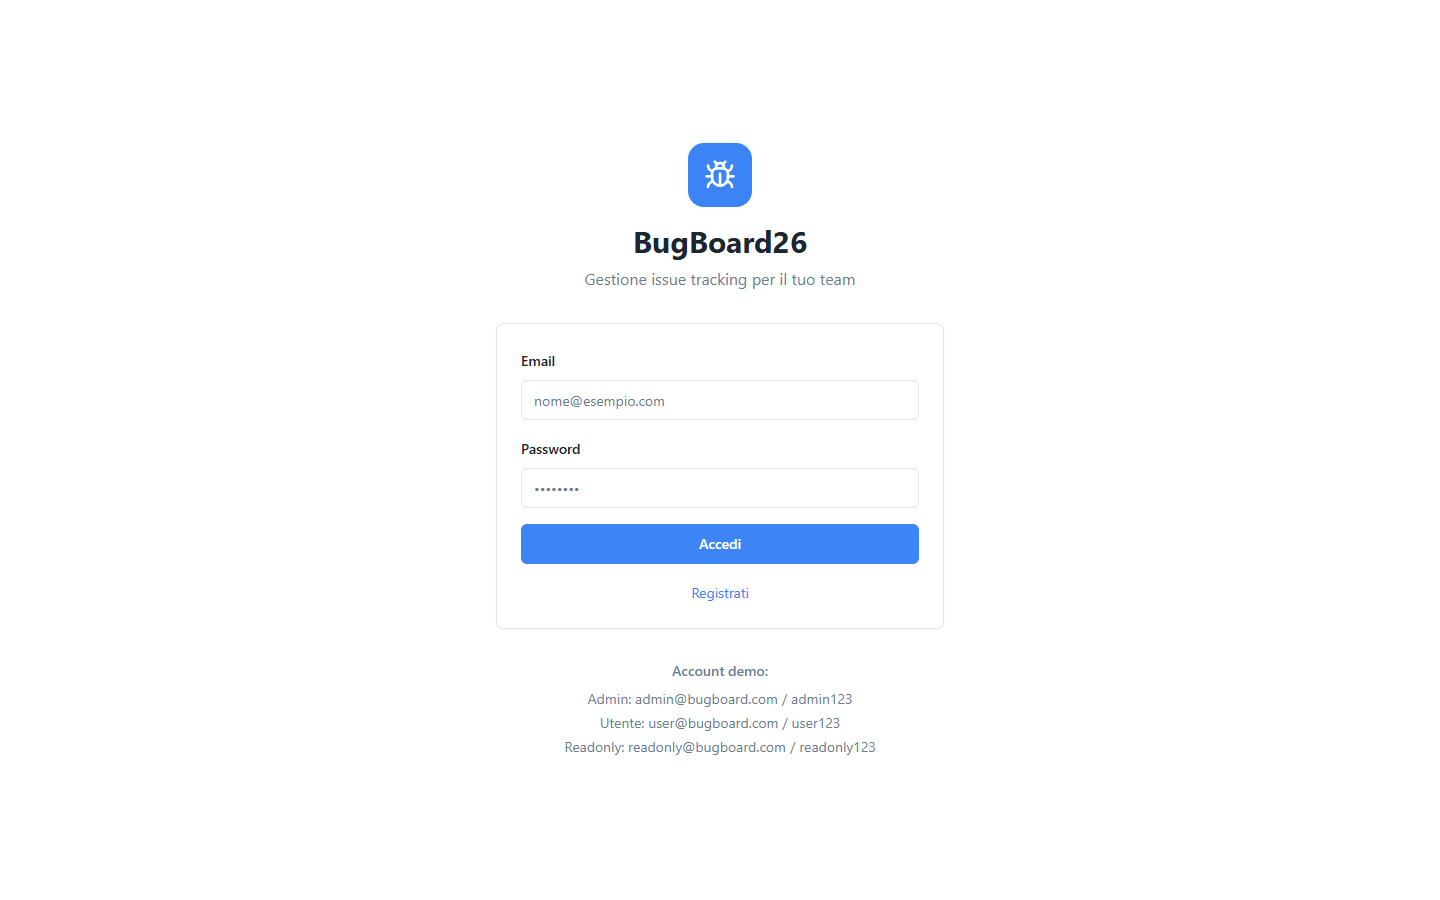
\includegraphics[width=0.85\textwidth]{immagini/mockup_08_notifiche.png}
    \caption{Centro Notifiche: lista degli aggiornamenti sui bug seguiti dall'utente}
    \label{fig:mockup_notifiche}
\end{figure}

\begin{itemize}
    \item \textbf{Scopo}: mostrare all'utente gli aggiornamenti recenti sui bug che lo riguardano (assegnazioni, cambi stato, nuovi commenti)
    \item \textbf{Elementi}: lista notifiche con timestamp, tipo evento e link al bug correlato; indicatore notifiche non lette
\end{itemize}

% ------- 9. PROFILO -------
\subsubsection{Mock-up 9 --- Profilo Utente}

\begin{figure}[H]
    \centering
    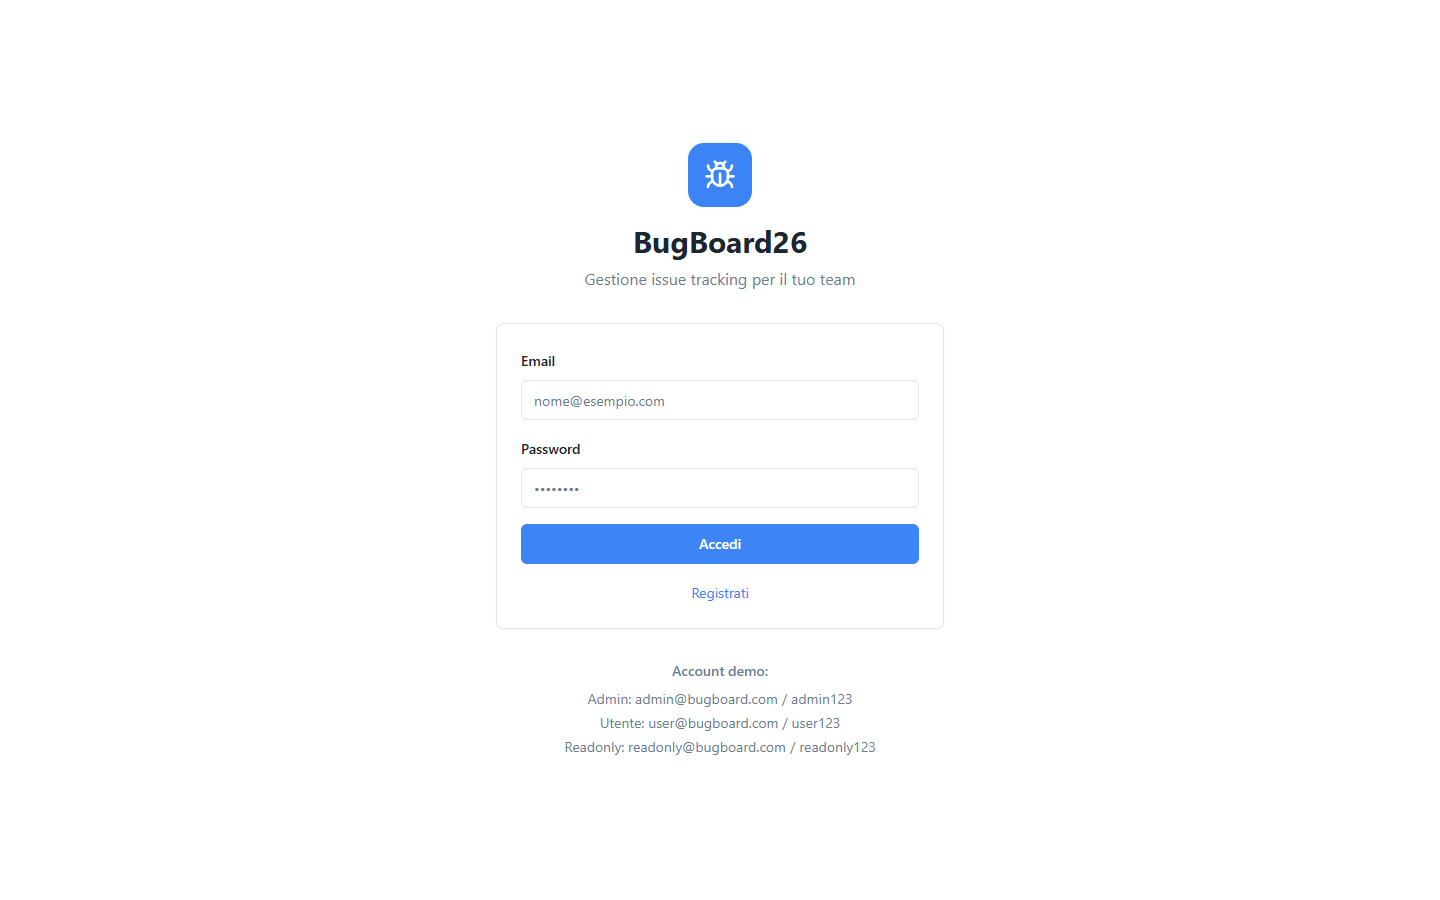
\includegraphics[width=0.85\textwidth]{immagini/mockup_09_profilo.png}
    \caption{Profilo Utente: gestione informazioni personali e cambio password}
    \label{fig:mockup_profilo}
\end{figure}

\begin{itemize}
    \item \textbf{Scopo}: consentire all'utente di visualizzare e modificare le proprie informazioni e la password
    \item \textbf{Elementi}: nome, email, ruolo (in sola lettura), form cambio password con validazione
\end{itemize}

% ------- 10. REPORT MENSILE (UC04) -------
\subsubsection{Mock-up 10 --- Report Mensile \textbf{[UC04]}}

\begin{figure}[H]
    \centering
    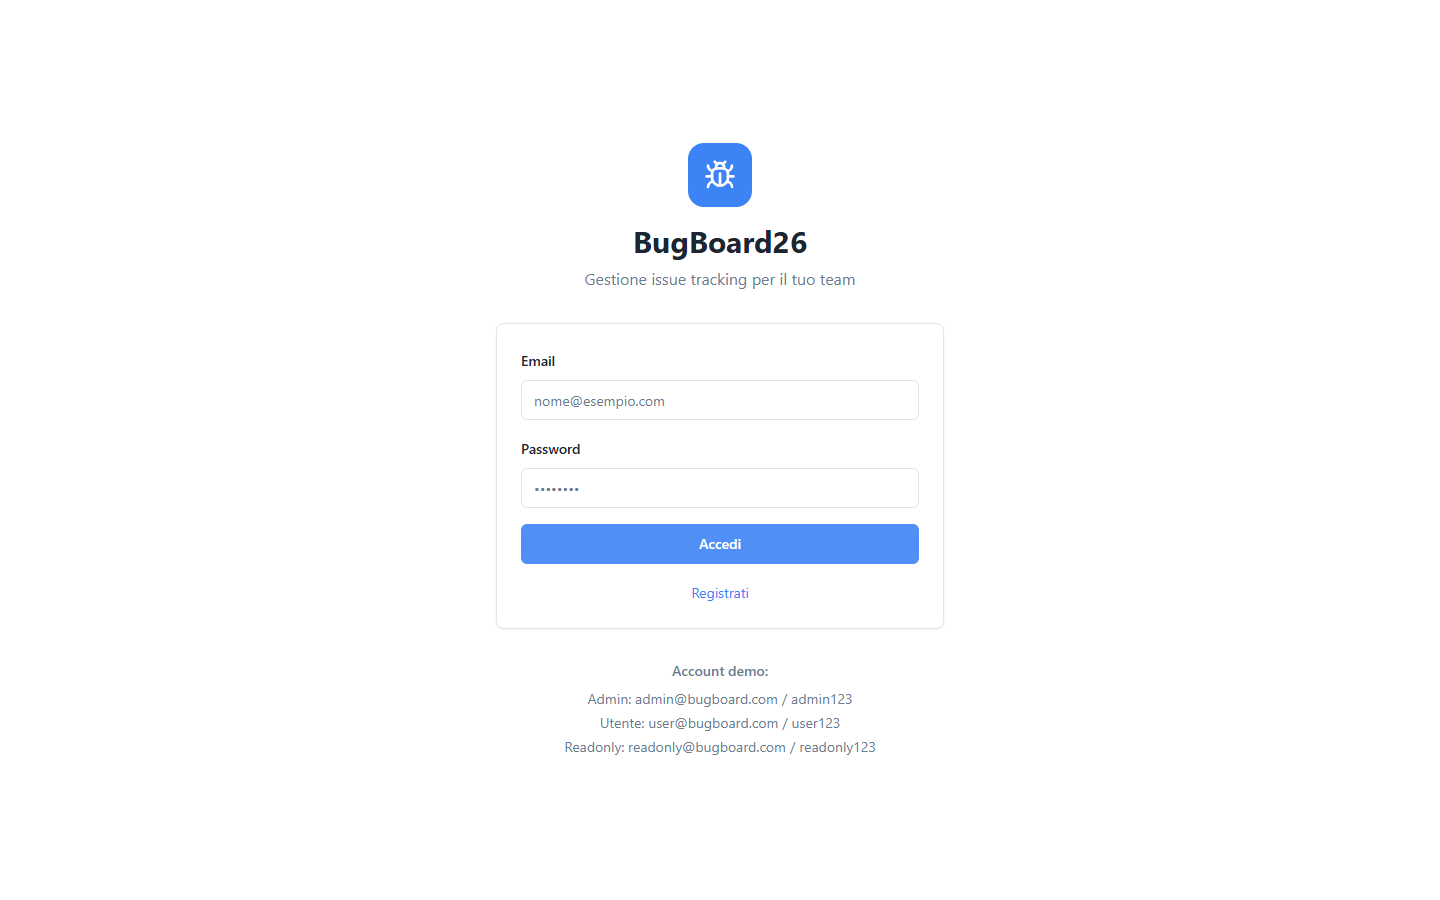
\includegraphics[width=0.85\textwidth]{immagini/mockup_10_report_mensile.png}
    \caption{Report Mensile Admin (UC04): statistiche, grafici e pulsante di export Excel}
    \label{fig:mockup_report}
\end{figure}

\begin{itemize}
    \item \textbf{Caso d'uso}: UC04 --- Generazione report mensile (solo Admin)
    \item \textbf{Elementi}: selettore mese/anno, grafici (distribuzione stato, priorità, trend temporale), tabella riassuntiva metriche, pulsante ``Esporta Excel''
    \item \textbf{Accesso}: solo Admin; gli altri utenti vengono reindirizzati alla Dashboard
\end{itemize}

% ------- 11. GESTIONE UTENTI ADMIN -------
\subsubsection{Mock-up 11 --- Gestione Utenti (Admin)}

\begin{figure}[H]
    \centering
    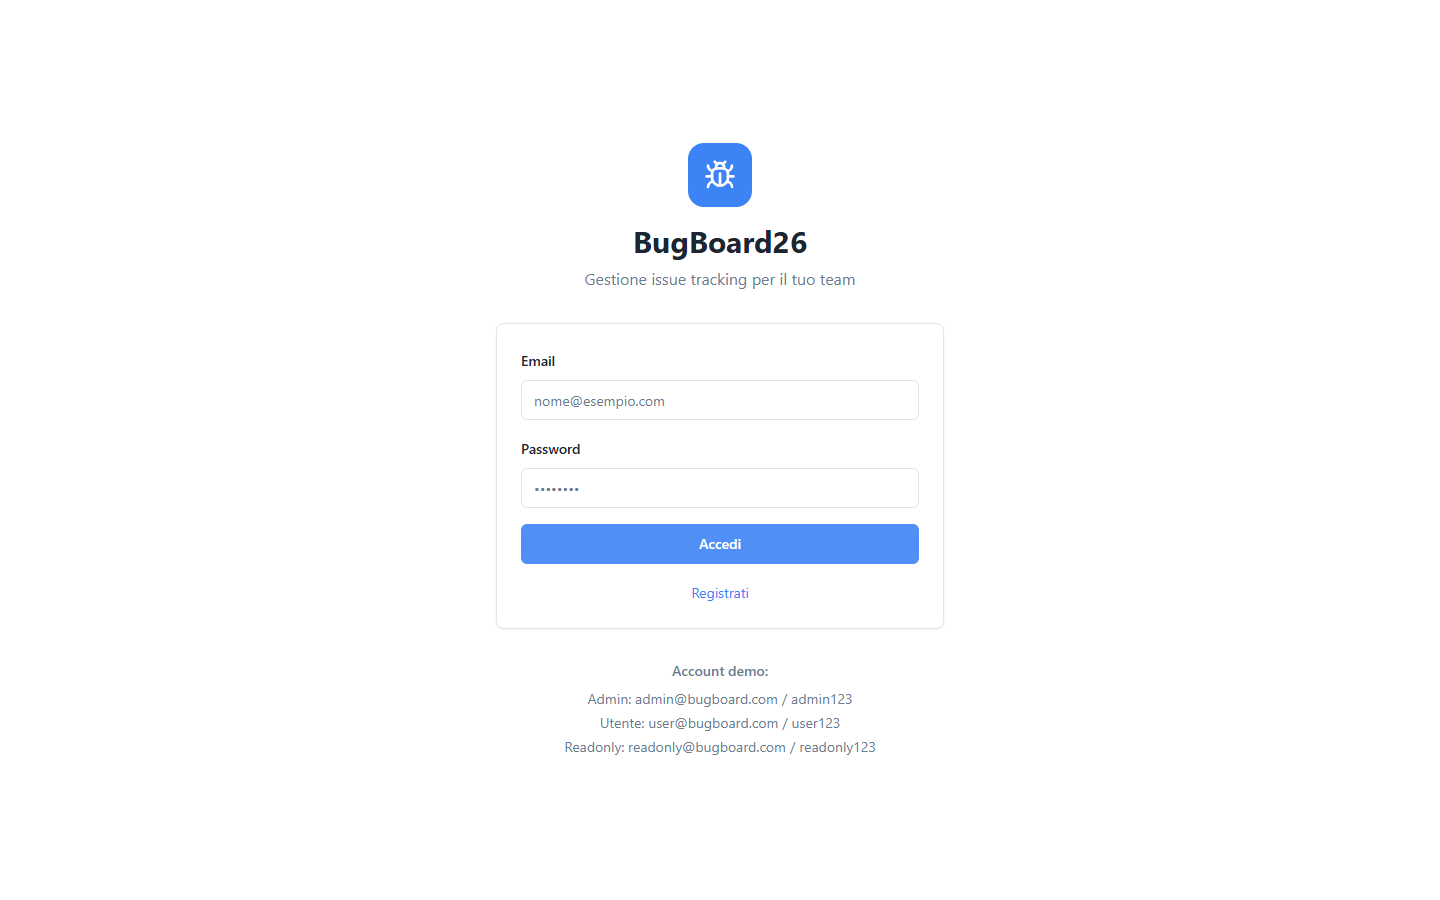
\includegraphics[width=0.85\textwidth]{immagini/mockup_11_admin_utenti.png}
    \caption{Gestione Utenti Admin: lista utenti con ruoli, stato e azioni di modifica}
    \label{fig:mockup_admin_utenti}
\end{figure}

\begin{itemize}
    \item \textbf{Scopo}: permettere all'Admin di gestire gli account del sistema (visualizzazione ruoli, disabilitazione utenti)
    \item \textbf{Elementi}: tabella utenti con email, nome, ruolo e stato; azioni per modifica ruolo e disabilitazione account
\end{itemize}

% ------- 12. ARCHIVIO -------
\subsubsection{Mock-up 12 --- Archivio Bug}

\begin{figure}[H]
    \centering
    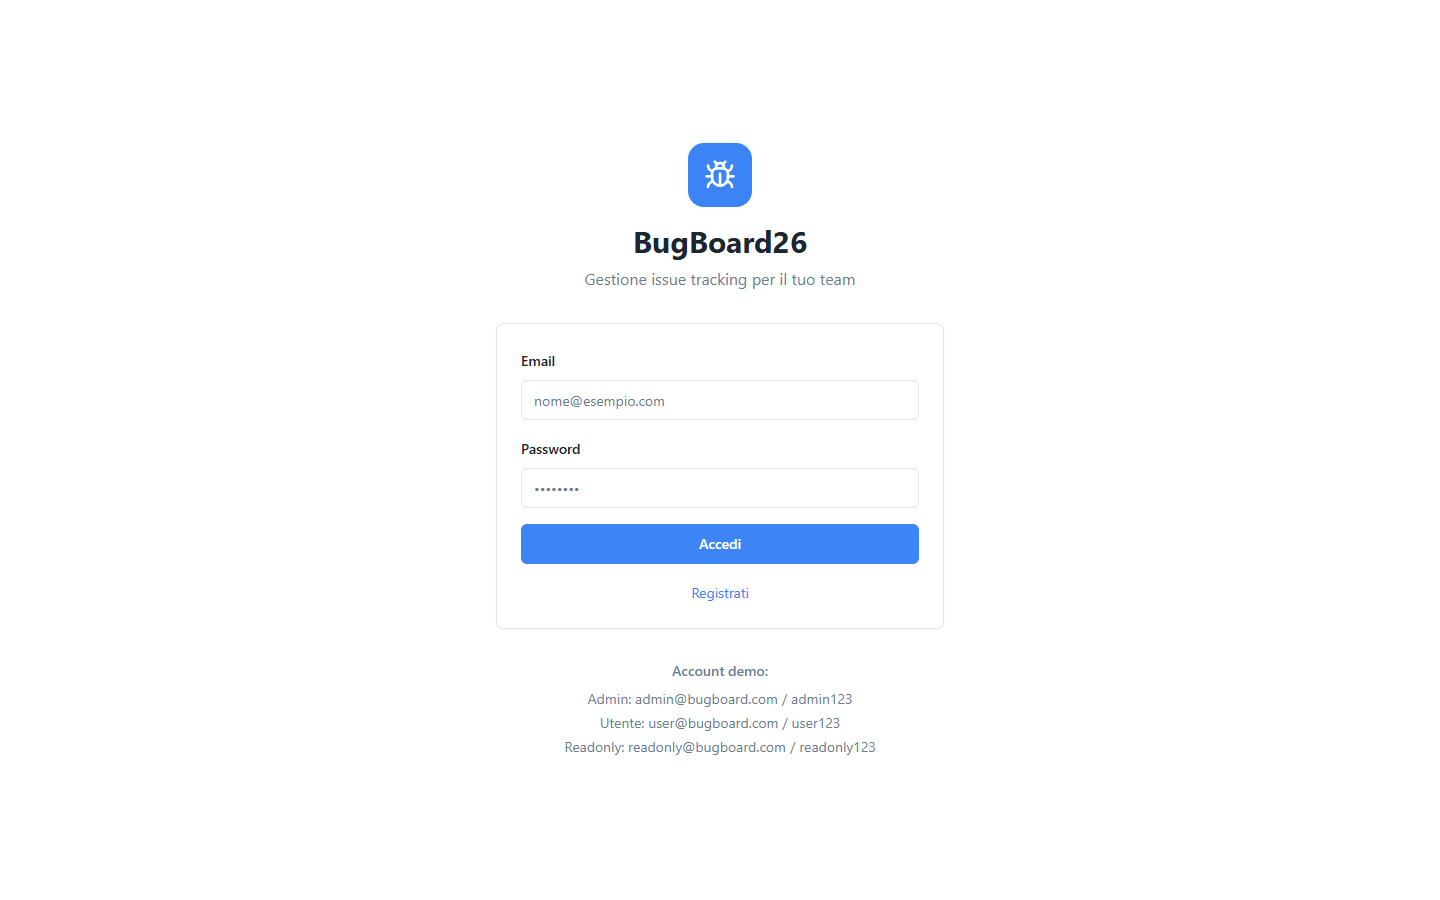
\includegraphics[width=0.85\textwidth]{immagini/mockup_12_archivio.png}
    \caption{Archivio Bug: lista dei bug archiviati con possibilità di consultazione}
    \label{fig:mockup_archivio}
\end{figure}

\begin{itemize}
    \item \textbf{Scopo}: visualizzare i bug archiviati per storico e consultazione senza influire sulla lista attiva
    \item \textbf{Elementi}: tabella bug in stato \textit{Archived} con filtri e ricerca; solo Admin può archiviare/ripristinare bug
\end{itemize}

% ------- 13. EXPORT -------
\subsubsection{Mock-up 13 --- Export Dati}

\begin{figure}[H]
    \centering
    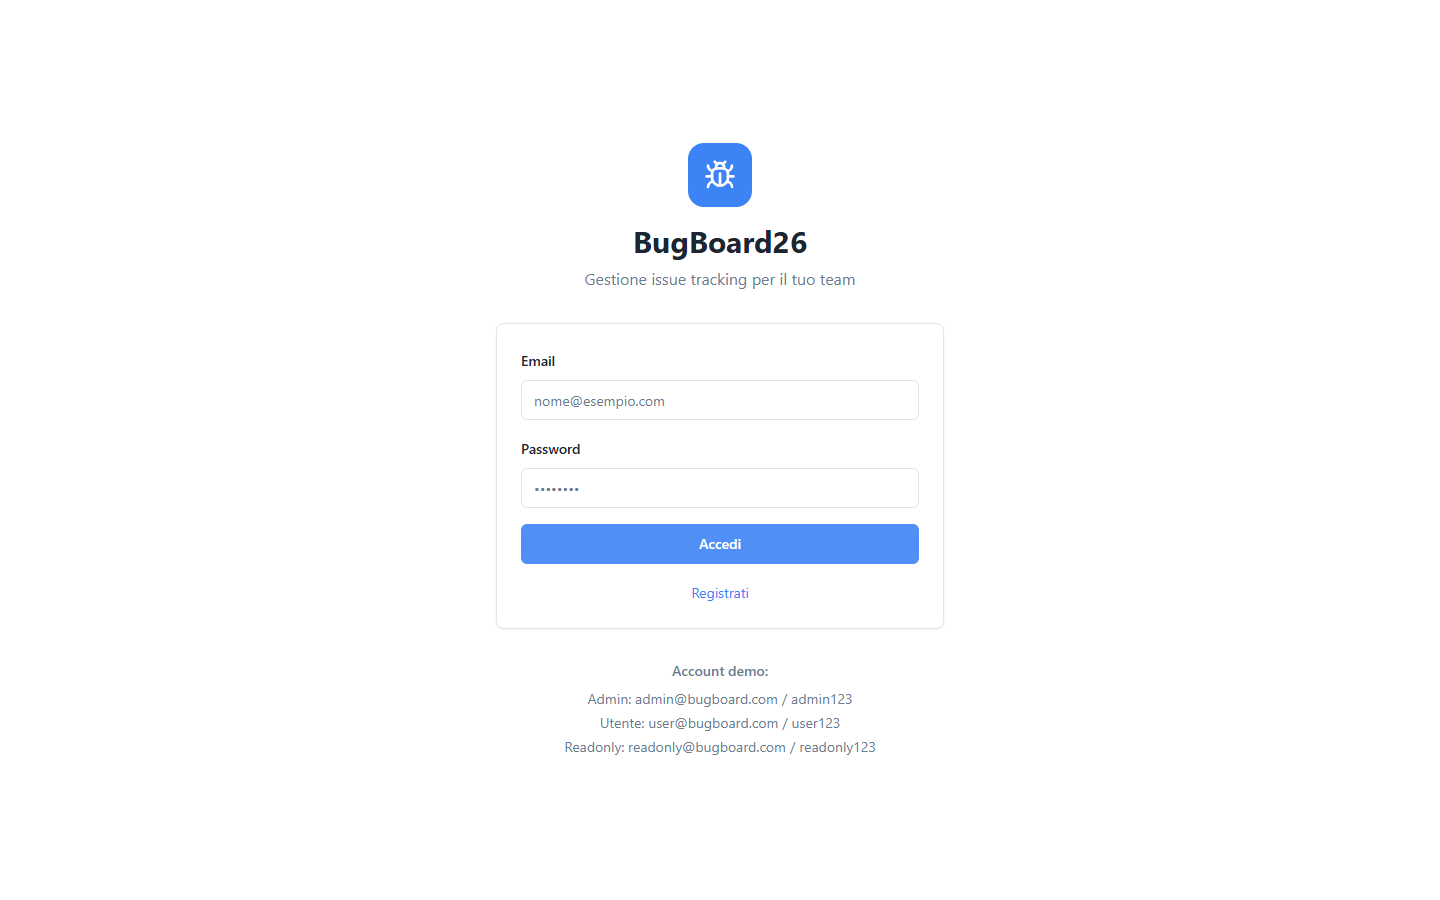
\includegraphics[width=0.85\textwidth]{immagini/mockup_13_export.png}
    \caption{Export Dati: download dell'elenco bug in formato CSV o Excel}
    \label{fig:mockup_export}
\end{figure}

\begin{itemize}
    \item \textbf{Scopo}: consentire l'esportazione dei dati per analisi esterne
    \item \textbf{Elementi}: pulsanti ``Scarica CSV'' e ``Scarica Excel''; i file vengono generati dal backend e scaricati direttamente
\end{itemize}

% ------------------------------------------------------------
\subsection{Osservazioni emerse dalla prototipazione}

La realizzazione del prototipo funzionante ha permesso di identificare alcune scelte migliorative rispetto all'analisi iniziale:

\begin{itemize}
    \item \textbf{Chiarezza dei ruoli}: è stato necessario rendere esplicito nel UI quali azioni sono riservate all'Admin (assegnazione, report, archiviazione, gestione utenti), aggiungendo reindirizzamenti automatici per utenti non autorizzati
    \item \textbf{Filtri immediati}: la lista bug con filtri in tempo reale si è rivelata la funzionalità più usata nelle sessioni di test, confermando la scelta di renderla la pagina principale
    \item \textbf{Badge colorati}: l'uso di badge cromatici per stato, priorità e tipo ha migliorato significativamente la leggibilità della lista bug senza aprire il dettaglio
    \item \textbf{Navigazione mobile}: il menu hamburger con le stesse voci del desktop ha garantito piena parità funzionale su dispositivi mobili
\end{itemize}

% ============================================================

\section{Prototipazione visuale attraverso Mock-up}

La prototipazione visuale di BugBoard26 è stata realizzata direttamente come applicazione React funzionante, con dati simulati (\textit{mock data}). Le schermate qui mostrate sono catture reali del prototipo interattivo, e non semplici bozzetti grafici. Questo approccio ha permesso di validare il flusso utente in modo concreto fin dalla fase di analisi.

% ------------------------------------------------------------
\subsection{Scelte Progettuali}

\subsubsection{Layout e Navigazione}
\begin{itemize}
    \item \textbf{Header fisso}: barra superiore con logo, link alle sezioni principali (Dashboard, Bug, Report, Admin) e menu utente con avatar, email e pulsante logout
    \item \textbf{Navigazione mobile}: menu a comparsa (hamburger) con le stesse voci, ottimizzato per touch
    \item \textbf{Layout responsive}: design \textit{mobile-first} realizzato con Tailwind CSS; le griglie si adattano automaticamente a qualsiasi larghezza schermo
\end{itemize}

\subsubsection{Palette Colori e Badge}
\begin{itemize}
    \item \textbf{Priorità}: \textit{Critical} (rosso), \textit{High} (arancione), \textit{Medium} (giallo), \textit{Low} (verde)
    \item \textbf{Stato}: \textit{Todo} (grigio chiaro), \textit{In Progress} (blu), \textit{Resolved} (verde), \textit{Archived} (grigio scuro)
    \item \textbf{Tipo}: \textit{Bug} (rosso), \textit{Feature} (viola), \textit{Enhancement} (azzurro)
    \item \textbf{Azioni primarie}: blu (\texttt{\#007BFF}); superfici neutre: grigi Tailwind
\end{itemize}

\subsubsection{Componenti UI riutilizzati}
Tutti i componenti sono basati su \textbf{Radix UI} e \textbf{shadcn/ui}: Button, Card, Select, Dialog, Badge, Table, Toast, DropdownMenu. Questo garantisce coerenza visiva e accessibilità WCAG 2.1 out-of-the-box.

% ------------------------------------------------------------
\subsection{Mock-up delle interfacce utente}

Di seguito sono illustrate le schermate principali del prototipo, raggruppate per funzionalità. Le schermate contrassegnate con \textbf{[UC0X]} corrispondono direttamente ai casi d'uso formalizzati nella sezione precedente.

% ------- 1. LOGIN -------
\subsubsection{Mock-up 1 --- Pagina di Login}

\begin{figure}[H]
    \centering
    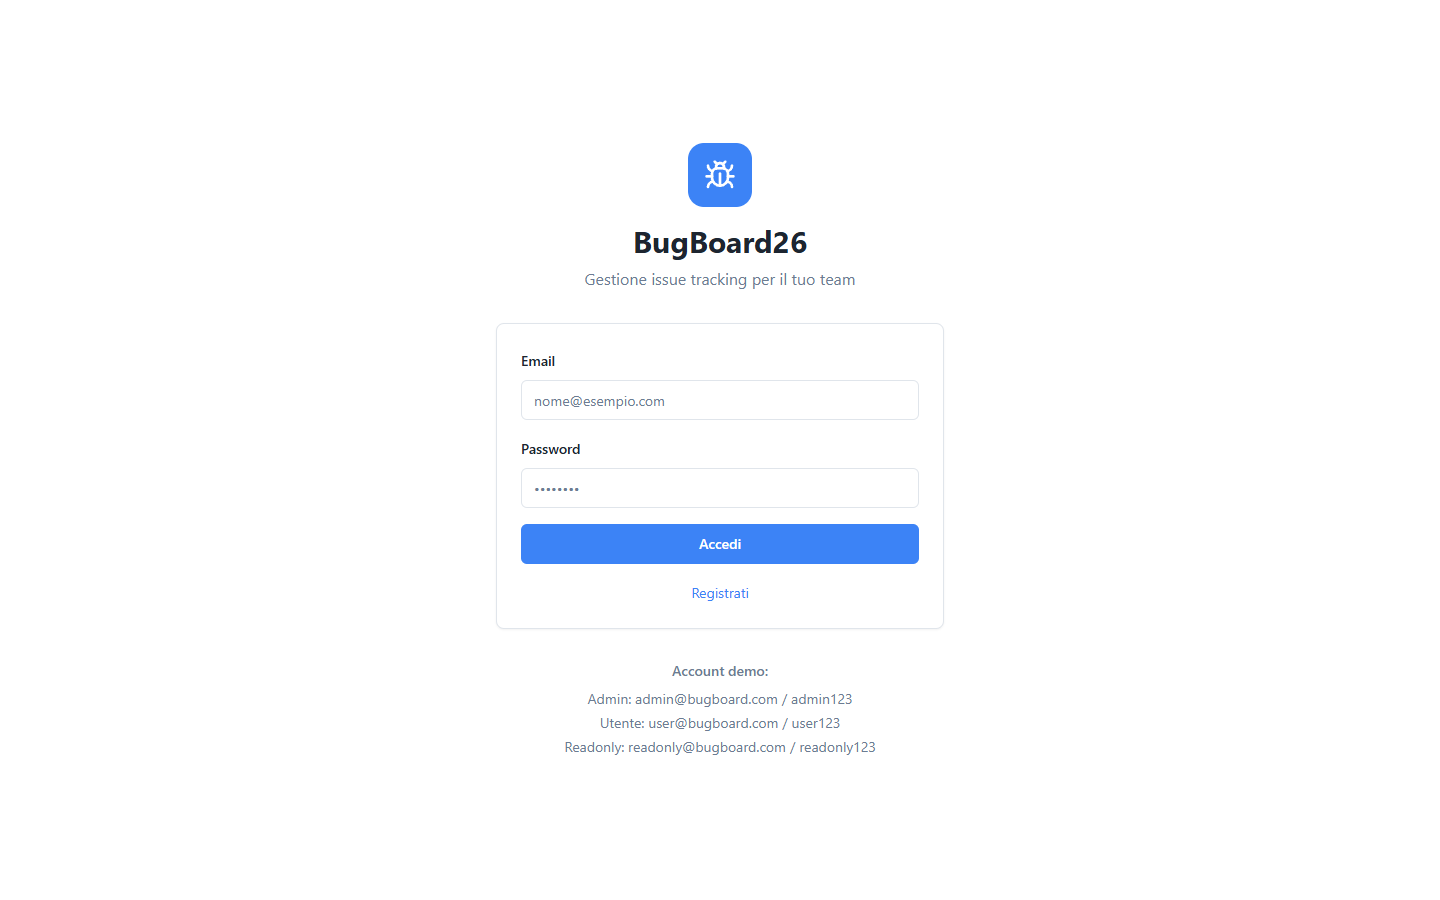
\includegraphics[width=0.85\textwidth]{immagini/mockup_01_login.png}
    \caption{Pagina di Login: form con email e password, pulsante di accesso}
    \label{fig:mockup_login}
\end{figure}

\begin{itemize}
    \item \textbf{Scopo}: autenticazione dell'utente al sistema
    \item \textbf{Elementi}: campo email, campo password, pulsante ``Accedi'', link alla pagina di registrazione
    \item \textbf{Comportamento}: in caso di credenziali errate viene mostrato un messaggio di errore inline; in caso di successo l'utente viene reindirizzato alla Dashboard
\end{itemize}

% ------- 2. REGISTRAZIONE -------
\subsubsection{Mock-up 2 --- Pagina di Registrazione}

\begin{figure}[H]
    \centering
    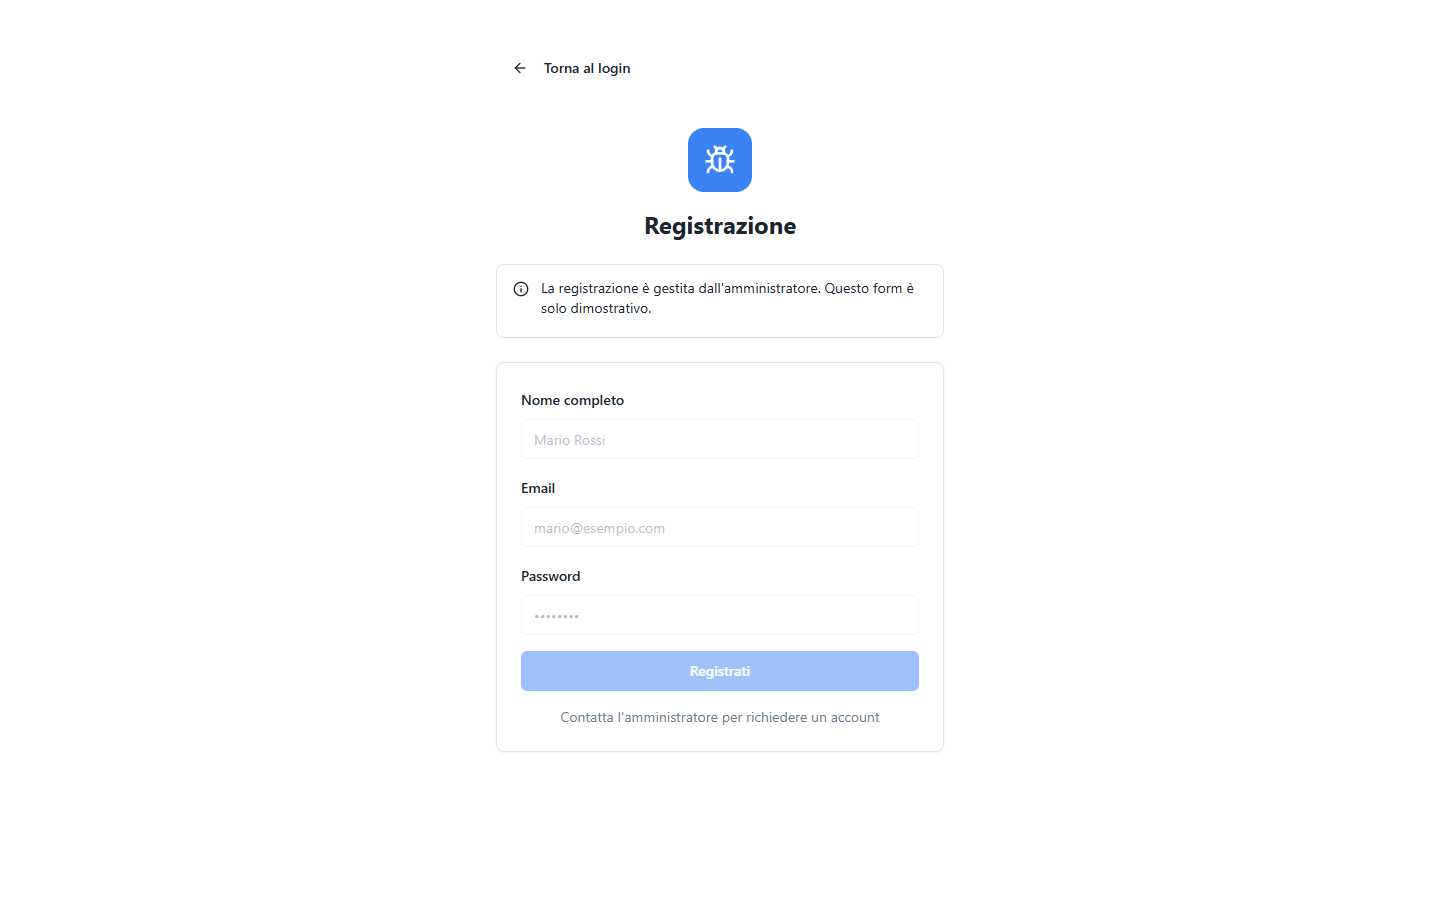
\includegraphics[width=0.85\textwidth]{immagini/mockup_02_register.png}
    \caption{Pagina di Registrazione: form con dati personali e creazione account}
    \label{fig:mockup_register}
\end{figure}

\begin{itemize}
    \item \textbf{Scopo}: creazione di un nuovo account utente
    \item \textbf{Elementi}: campi nome, email, password, conferma password; pulsante ``Registrati''
    \item \textbf{Validazione}: i campi vengono validati in tempo reale con messaggi di errore inline
\end{itemize}

% ------- 3. HOME -------
\subsubsection{Mock-up 3 --- Home / Dashboard}

\begin{figure}[H]
    \centering
    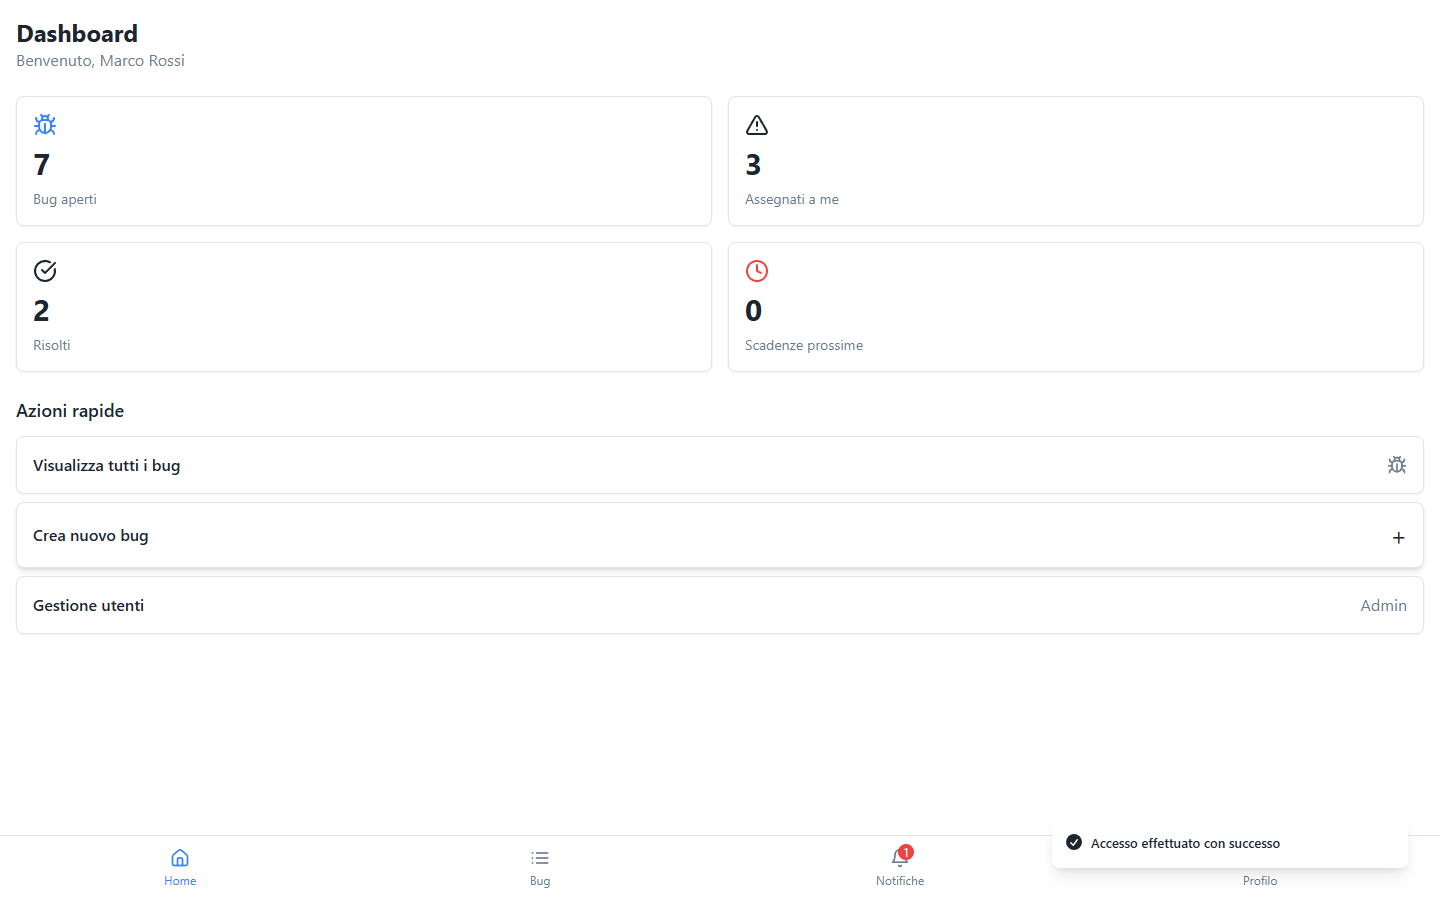
\includegraphics[width=0.85\textwidth]{immagini/mockup_03_home_dashboard.png}
    \caption{Home Dashboard: panoramica delle metriche principali e accessi rapidi}
    \label{fig:mockup_home}
\end{figure}

\begin{itemize}
    \item \textbf{Scopo}: fornire una panoramica immediata dello stato del sistema dopo il login
    \item \textbf{Elementi}: card metriche (bug aperti, assegnati a me, risolti, scadenze prossime), header con navigazione principale
    \item \textbf{Accessi rapidi}: da qui si può navigare alla lista bug, al form di creazione e ai report
\end{itemize}

% ------- 4. LISTA BUG -------
\subsubsection{Mock-up 4 --- Lista Bug con Filtri}

\begin{figure}[H]
    \centering
    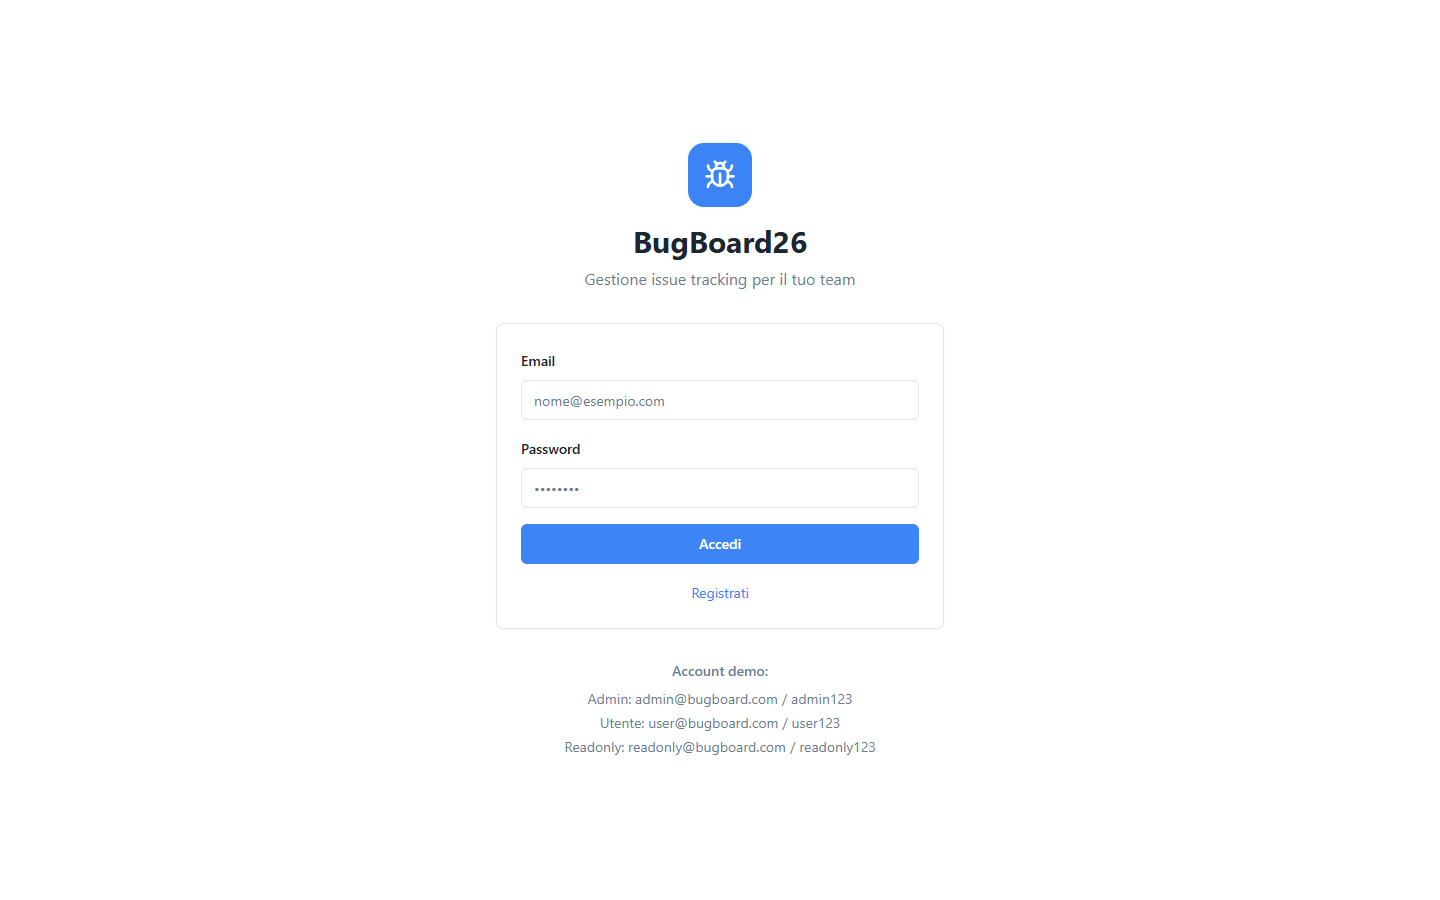
\includegraphics[width=0.85\textwidth]{immagini/mockup_04_lista_bug.png}
    \caption{Lista Bug: tabella con filtri per tipo, stato, priorità e ricerca testuale}
    \label{fig:mockup_lista_bug}
\end{figure}

\begin{itemize}
    \item \textbf{Scopo}: visualizzazione e filtraggio dell'elenco completo dei bug
    \item \textbf{Elementi}: barra filtri orizzontale (tipo, stato, priorità), campo ricerca full-text, tabella bug con badge colorati, paginazione
    \item \textbf{Interazione}: clic su una riga apre il dettaglio del bug; i filtri si applicano in tempo reale
\end{itemize}

% ------- 5. DETTAGLIO BUG -------
\subsubsection{Mock-up 5 --- Dettaglio Bug}

\begin{figure}[H]
    \centering
    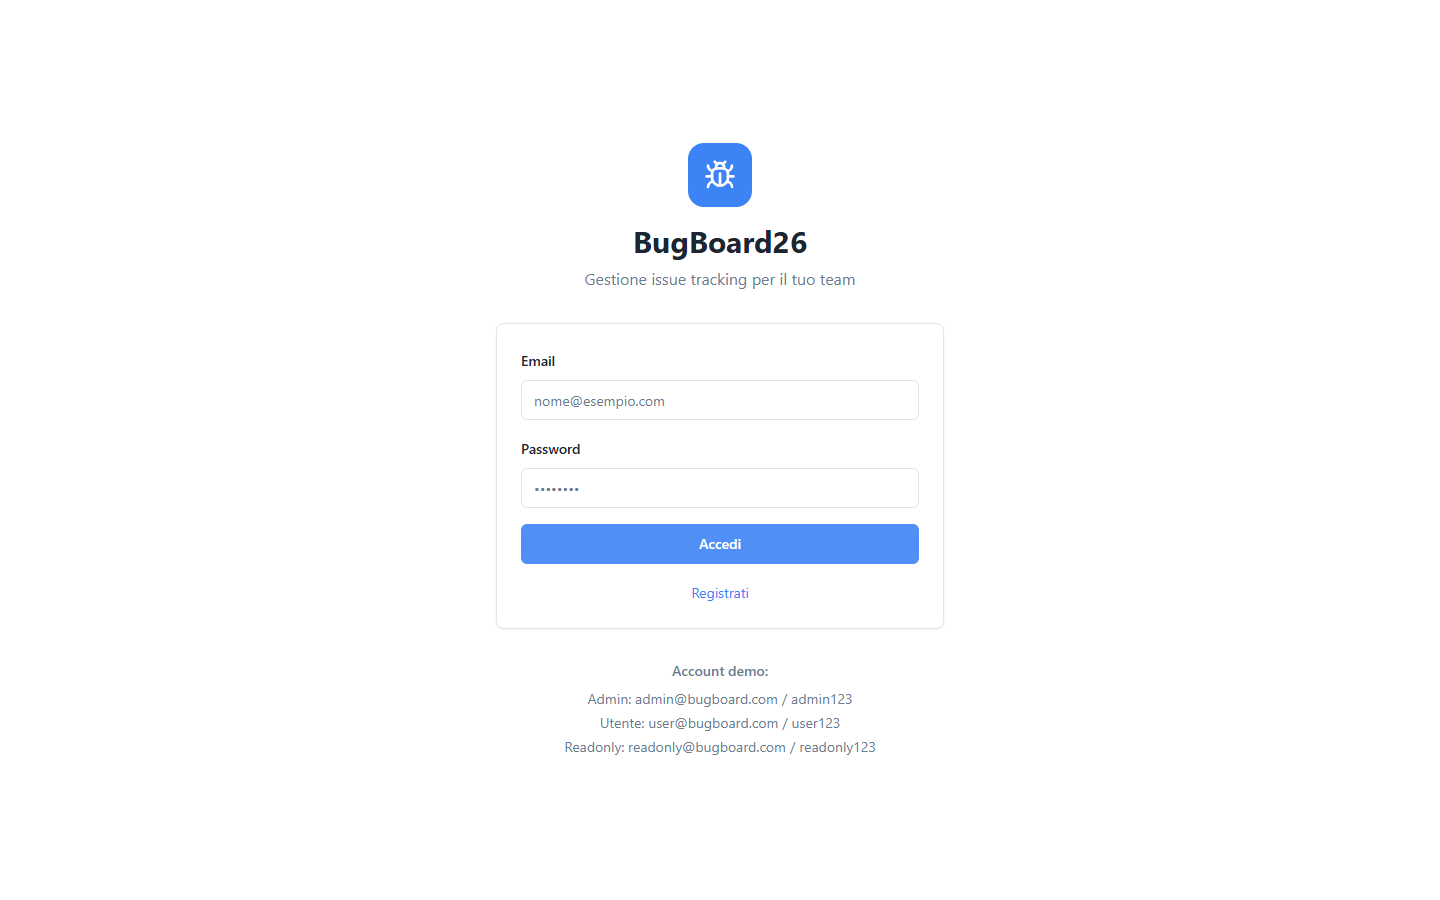
\includegraphics[width=0.85\textwidth]{immagini/mockup_05_dettaglio_bug.png}
    \caption{Dettaglio Bug: informazioni complete, commenti, storico modifiche e azioni disponibili}
    \label{fig:mockup_dettaglio_bug}
\end{figure}

\begin{itemize}
    \item \textbf{Scopo}: visualizzazione completa di un bug specifico e gestione delle azioni disponibili
    \item \textbf{Elementi}: header con titolo, stato e priorità; sezioni descrizione, commenti, allegati, storico; barra azioni laterale (modifica, assegna, risolvi, archivia, duplica)
    \item \textbf{Azioni visibili}: dipendono dal ruolo dell'utente (USER vede meno azioni rispetto ad Admin)
\end{itemize}

% ------- 6. FORM CREAZIONE BUG (UC01) -------
\subsubsection{Mock-up 6 --- Form Creazione/Modifica Bug \textbf{[UC01]}}

\begin{figure}[H]
    \centering
    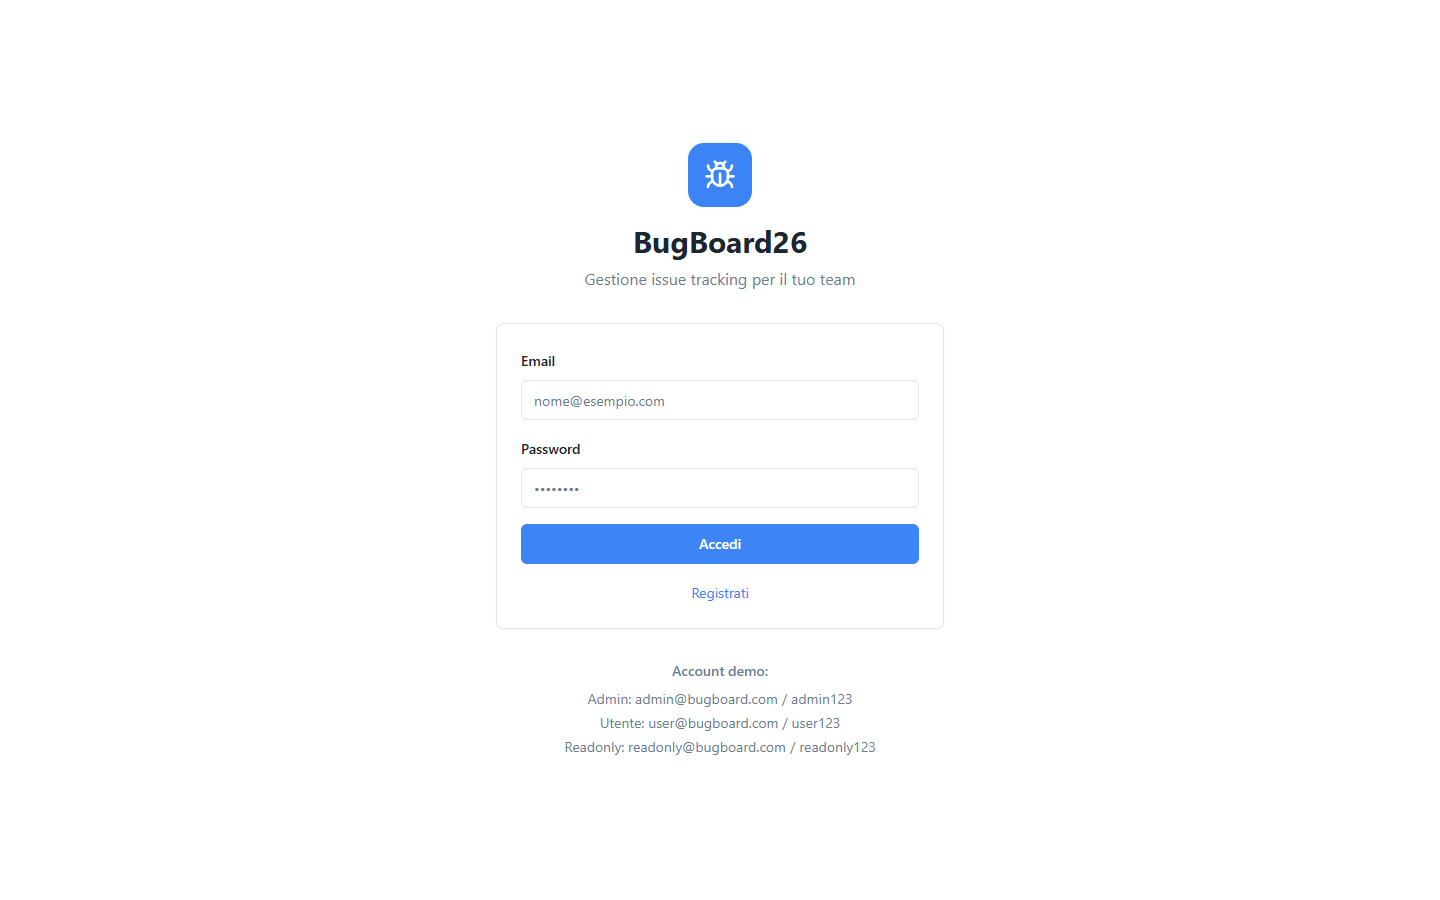
\includegraphics[width=0.85\textwidth]{immagini/mockup_06_form_creazione_bug.png}
    \caption{Form Creazione Bug (UC01): campi titolo, tipo, priorità, descrizione, label, allegati}
    \label{fig:mockup_form_bug}
\end{figure}

\begin{itemize}
    \item \textbf{Caso d'uso}: UC01 --- Creazione nuovo bug
    \item \textbf{Elementi}: campo titolo, selettori tipo e priorità, area di testo descrizione, selezione label multipla, upload allegati immagine, selezione assegnatario opzionale, pulsante ``Salva''
    \item \textbf{Validazione}: i campi obbligatori (titolo, tipo, priorità) sono evidenziati se lasciati vuoti; il formato e la dimensione degli allegati sono verificati prima dell'invio
\end{itemize}

% ------- 7. ASSEGNAZIONE BUG (UC02) -------
\subsubsection{Mock-up 7 --- Assegnazione Bug \textbf{[UC02]}}

\begin{figure}[H]
    \centering
    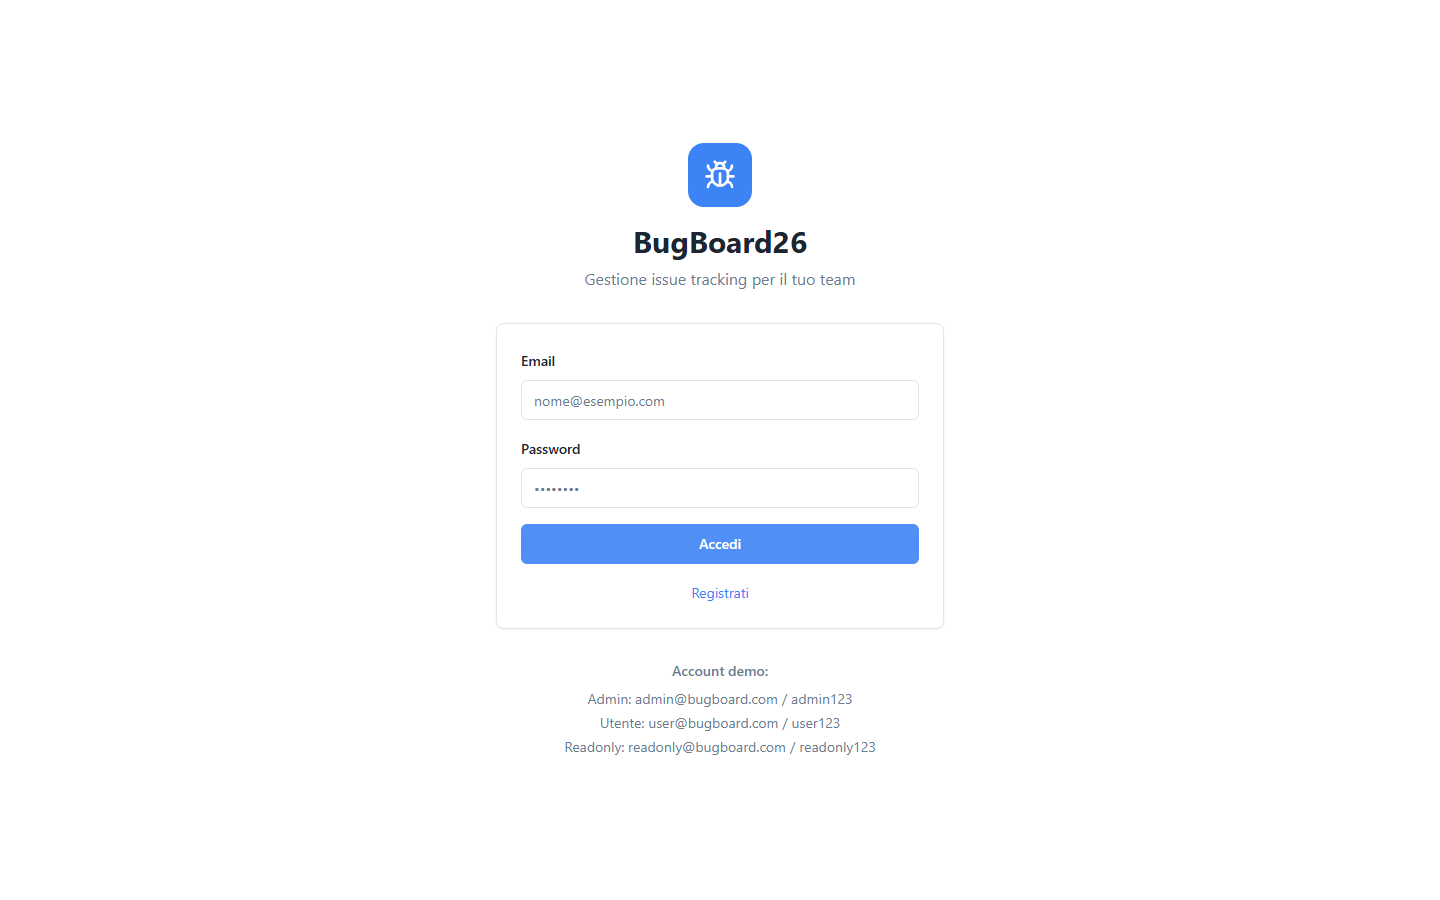
\includegraphics[width=0.85\textwidth]{immagini/mockup_07_assegnazione_bug.png}
    \caption{Assegnazione Bug (UC02): selezione dell'utente a cui assegnare il bug}
    \label{fig:mockup_assegnazione}
\end{figure}

\begin{itemize}
    \item \textbf{Caso d'uso}: UC02 --- Assegnazione bug a un utente (solo Admin)
    \item \textbf{Elementi}: select per la scelta dell'utente assegnatario, pulsante conferma
    \item \textbf{Accesso}: questa schermata è accessibile solo agli utenti con ruolo Admin; un USER viene reindirizzato alla Dashboard
\end{itemize}

% ------- 8. NOTIFICHE -------
\subsubsection{Mock-up 8 --- Notifiche}

\begin{figure}[H]
    \centering
    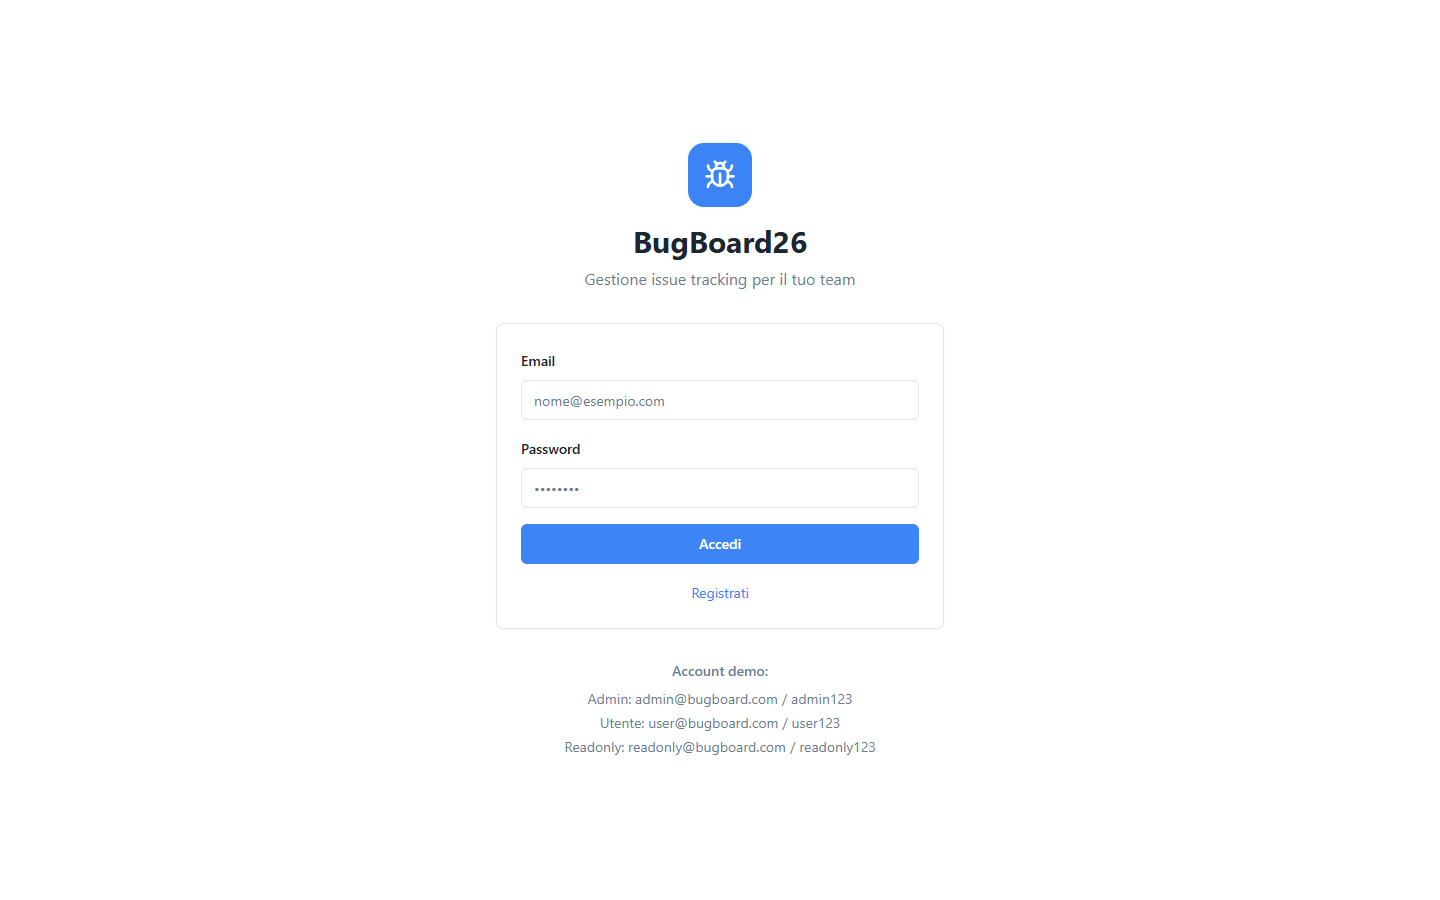
\includegraphics[width=0.85\textwidth]{immagini/mockup_08_notifiche.png}
    \caption{Centro Notifiche: lista degli aggiornamenti sui bug seguiti dall'utente}
    \label{fig:mockup_notifiche}
\end{figure}

\begin{itemize}
    \item \textbf{Scopo}: mostrare all'utente gli aggiornamenti recenti sui bug che lo riguardano (assegnazioni, cambi stato, nuovi commenti)
    \item \textbf{Elementi}: lista notifiche con timestamp, tipo evento e link al bug correlato; indicatore notifiche non lette
\end{itemize}

% ------- 9. PROFILO -------
\subsubsection{Mock-up 9 --- Profilo Utente}

\begin{figure}[H]
    \centering
    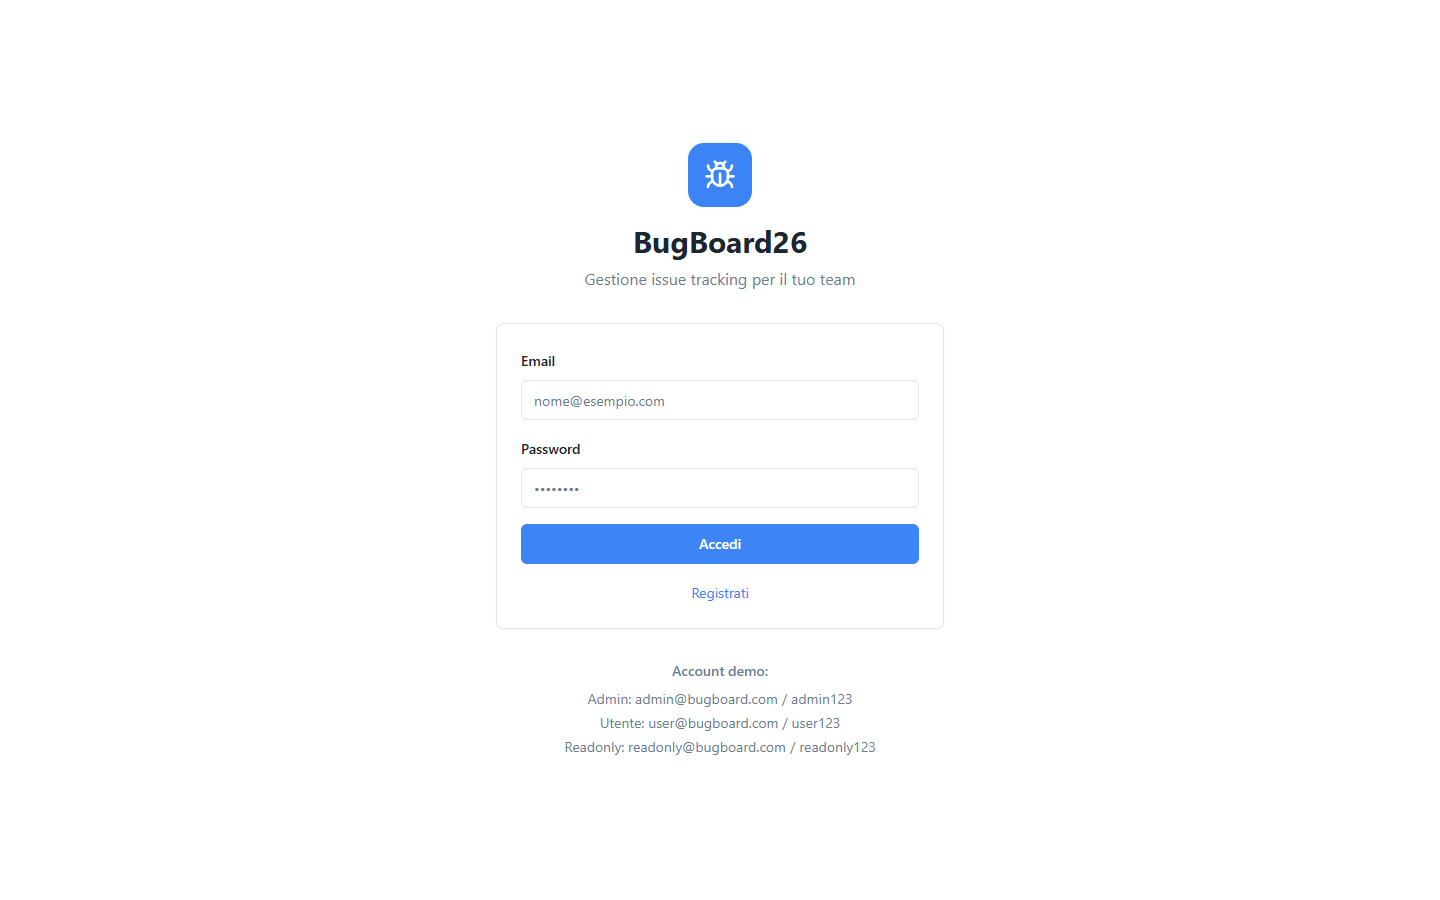
\includegraphics[width=0.85\textwidth]{immagini/mockup_09_profilo.png}
    \caption{Profilo Utente: gestione informazioni personali e cambio password}
    \label{fig:mockup_profilo}
\end{figure}

\begin{itemize}
    \item \textbf{Scopo}: consentire all'utente di visualizzare e modificare le proprie informazioni e la password
    \item \textbf{Elementi}: nome, email, ruolo (in sola lettura), form cambio password con validazione
\end{itemize}

% ------- 10. REPORT MENSILE (UC04) -------
\subsubsection{Mock-up 10 --- Report Mensile \textbf{[UC04]}}

\begin{figure}[H]
    \centering
    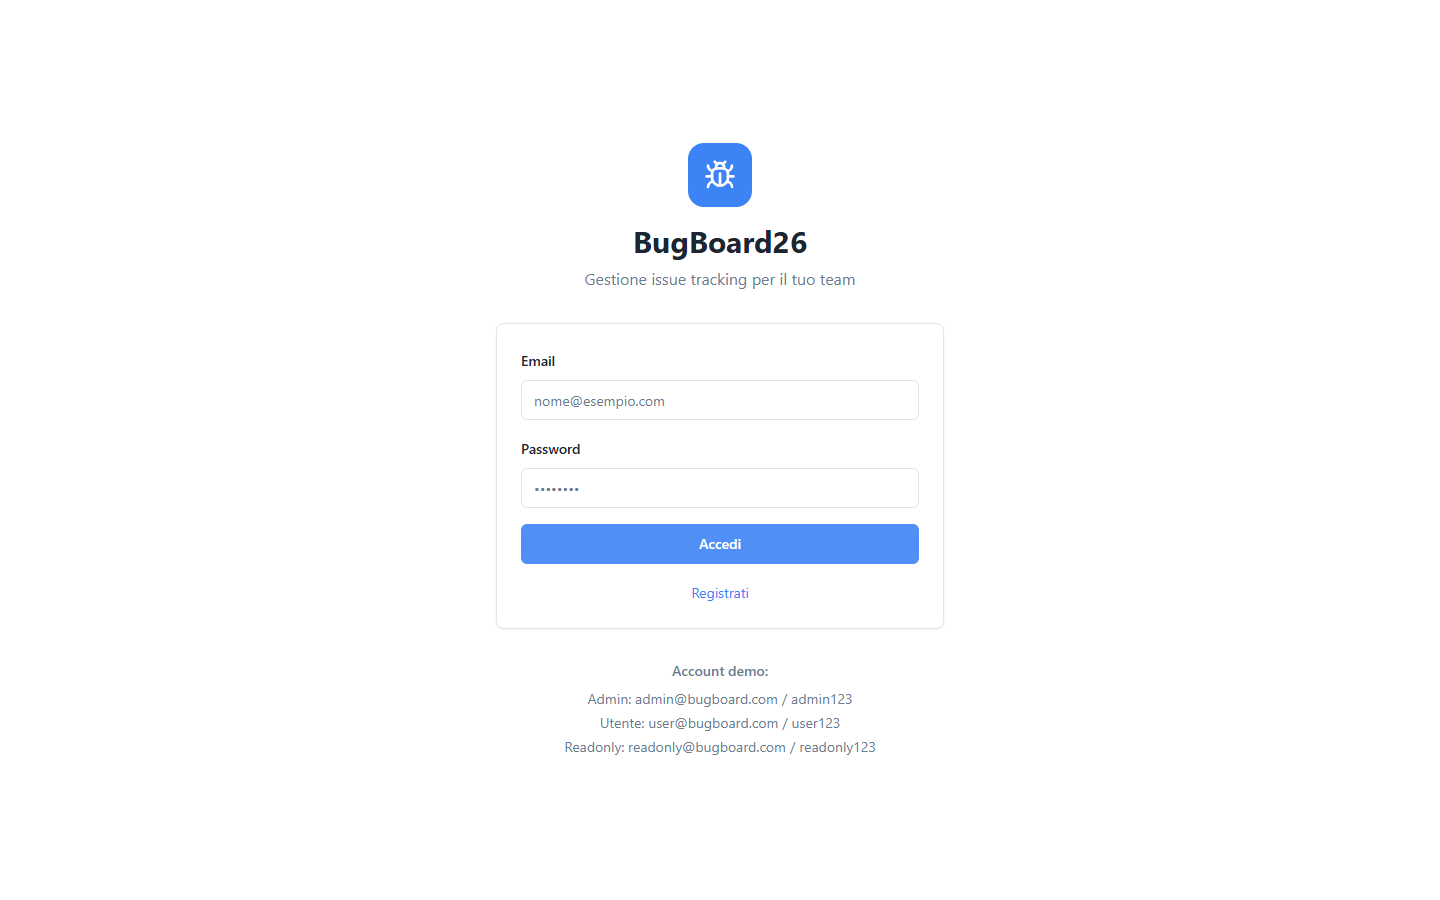
\includegraphics[width=0.85\textwidth]{immagini/mockup_10_report_mensile.png}
    \caption{Report Mensile Admin (UC04): statistiche, grafici e pulsante di export Excel}
    \label{fig:mockup_report}
\end{figure}

\begin{itemize}
    \item \textbf{Caso d'uso}: UC04 --- Generazione report mensile (solo Admin)
    \item \textbf{Elementi}: selettore mese/anno, grafici (distribuzione stato, priorità, trend temporale), tabella riassuntiva metriche, pulsante ``Esporta Excel''
    \item \textbf{Accesso}: solo Admin; gli altri utenti vengono reindirizzati alla Dashboard
\end{itemize}

% ------- 11. GESTIONE UTENTI ADMIN -------
\subsubsection{Mock-up 11 --- Gestione Utenti (Admin)}

\begin{figure}[H]
    \centering
    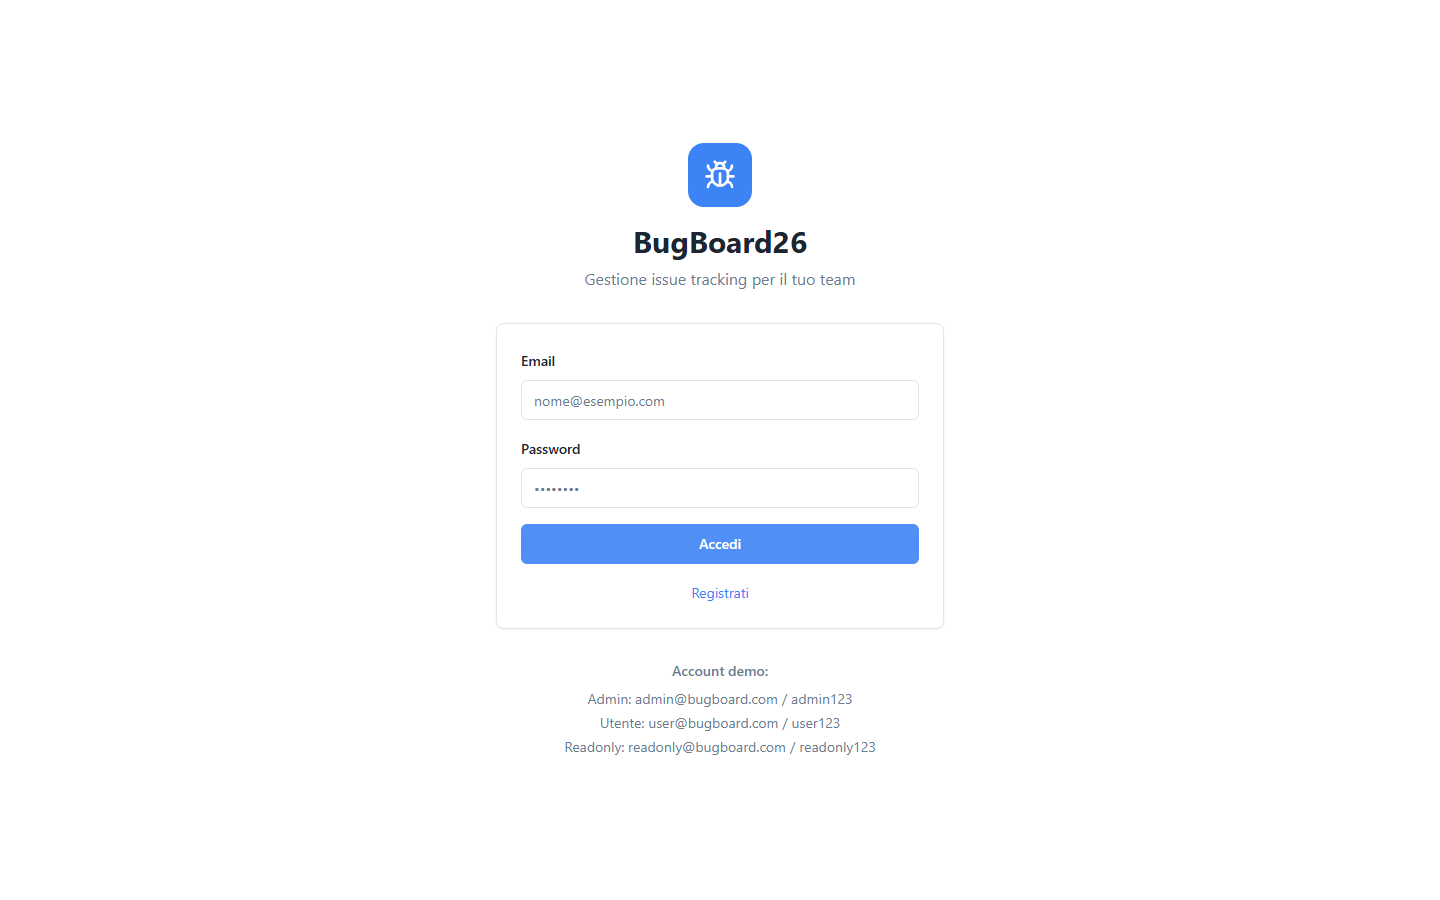
\includegraphics[width=0.85\textwidth]{immagini/mockup_11_admin_utenti.png}
    \caption{Gestione Utenti Admin: lista utenti con ruoli, stato e azioni di modifica}
    \label{fig:mockup_admin_utenti}
\end{figure}

\begin{itemize}
    \item \textbf{Scopo}: permettere all'Admin di gestire gli account del sistema (visualizzazione ruoli, disabilitazione utenti)
    \item \textbf{Elementi}: tabella utenti con email, nome, ruolo e stato; azioni per modifica ruolo e disabilitazione account
\end{itemize}

% ------- 12. ARCHIVIO -------
\subsubsection{Mock-up 12 --- Archivio Bug}

\begin{figure}[H]
    \centering
    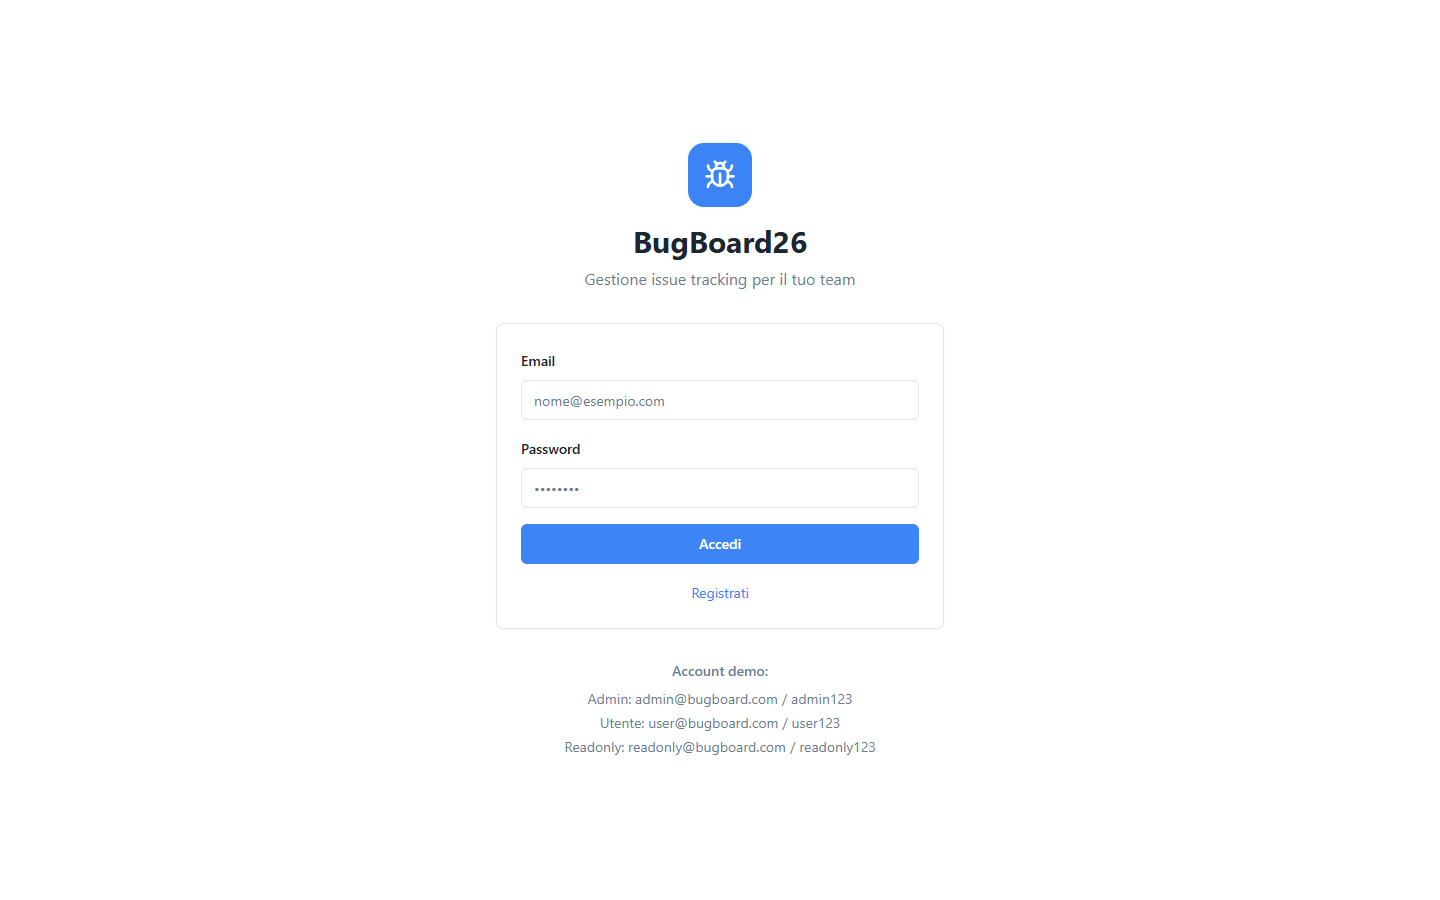
\includegraphics[width=0.85\textwidth]{immagini/mockup_12_archivio.png}
    \caption{Archivio Bug: lista dei bug archiviati con possibilità di consultazione}
    \label{fig:mockup_archivio}
\end{figure}

\begin{itemize}
    \item \textbf{Scopo}: visualizzare i bug archiviati per storico e consultazione senza influire sulla lista attiva
    \item \textbf{Elementi}: tabella bug in stato \textit{Archived} con filtri e ricerca; solo Admin può archiviare/ripristinare bug
\end{itemize}

% ------- 13. EXPORT -------
\subsubsection{Mock-up 13 --- Export Dati}

\begin{figure}[H]
    \centering
    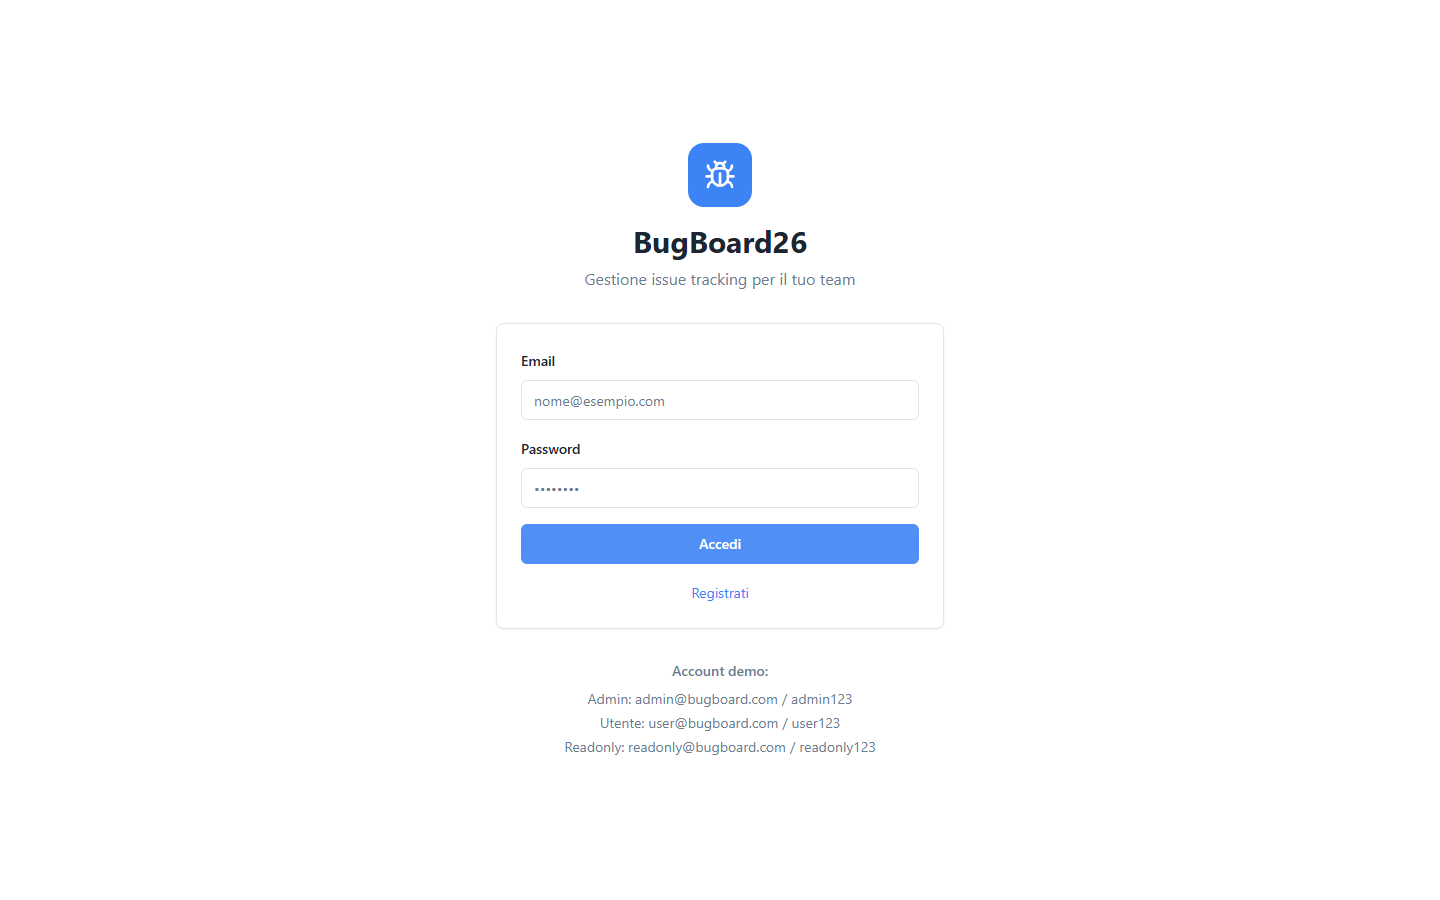
\includegraphics[width=0.85\textwidth]{immagini/mockup_13_export.png}
    \caption{Export Dati: download dell'elenco bug in formato CSV o Excel}
    \label{fig:mockup_export}
\end{figure}

\begin{itemize}
    \item \textbf{Scopo}: consentire l'esportazione dei dati per analisi esterne
    \item \textbf{Elementi}: pulsanti ``Scarica CSV'' e ``Scarica Excel''; i file vengono generati dal backend e scaricati direttamente
\end{itemize}

% ------------------------------------------------------------
\subsection{Osservazioni emerse dalla prototipazione}

La realizzazione del prototipo funzionante ha permesso di identificare alcune scelte migliorative rispetto all'analisi iniziale:

\begin{itemize}
    \item \textbf{Chiarezza dei ruoli}: è stato necessario rendere esplicito nel UI quali azioni sono riservate all'Admin (assegnazione, report, archiviazione, gestione utenti), aggiungendo reindirizzamenti automatici per utenti non autorizzati
    \item \textbf{Filtri immediati}: la lista bug con filtri in tempo reale si è rivelata la funzionalità più usata nelle sessioni di test, confermando la scelta di renderla la pagina principale
    \item \textbf{Badge colorati}: l'uso di badge cromatici per stato, priorità e tipo ha migliorato significativamente la leggibilità della lista bug senza aprire il dettaglio
    \item \textbf{Navigazione mobile}: il menu hamburger con le stesse voci del desktop ha garantito piena parità funzionale su dispositivi mobili
\end{itemize}


% ============================================================
% DESIGN DEL SISTEMA
% design_sistema.tex — Documento di Design del Sistema

\section{Design del Sistema}

\subsection{Descrizione dell'architettura}

BugBoard26 adotta un'architettura \textbf{client-server a tre livelli}
(Three-Tier Architecture), separando nettamente le responsabilità tra
\emph{presentazione}, \emph{logica di business} e \emph{persistenza dei dati}.

\begin{center}
\begin{tabular}{|l|p{10cm}|}
\hline
\textbf{Livello} & \textbf{Descrizione} \\
\hline
Presentazione (Frontend) & Single Page Application React che comunica con il backend tramite API REST. \\
\hline
Logica di Business (Backend) & Applicazione Spring Boot che espone endpoint RESTful, gestisce autenticazione JWT e implementa le regole di business. \\
\hline
Persistenza (Database) & Database relazionale (H2 in sviluppo, PostgreSQL in produzione) gestito tramite JPA/Hibernate. \\
\hline
\end{tabular}
\end{center}

\subsubsection{Diagramma architetturale}

\begin{verbatim}
  +-----------------+       HTTPS/REST       +-------------------+
  |                 |  <------------------->  |                   |
  |    Frontend     |       /api/*           |     Backend       |
  |    (React SPA)  |                        |   (Spring Boot)   |
  |    Port 8080    |                        |    Port 8081      |
  +-----------------+                        +--------+----------+
        |                                             |
        | (Vite dev proxy)                            | JPA/Hibernate
        | /api -> localhost:8081                       |
        |                                    +--------v----------+
        |                                    |                   |
        |                                    |     Database      |
        |                                    |  H2 / PostgreSQL  |
        |                                    +-------------------+
        |
        v
  +-----------------+
  | Docker Compose  |
  |  (Produzione)   |
  +-----------------+
\end{verbatim}

\subsection{Criteri di design adottati}

\begin{description}
    \item[Separazione delle responsabilità (\emph{Separation of Concerns})]
    Ogni livello ha una responsabilità ben definita: il frontend si occupa
    esclusivamente della presentazione e dell'interazione utente, il backend
    della logica di business e dell'autorizzazione, il database della
    persistenza. Questa separazione favorisce la manutenibilità e la
    testabilità.

    \item[Stateless Authentication]
    L'autenticazione è gestita tramite token JWT, eliminando la necessità
    di sessioni server-side. Ogni richiesta contiene il token necessario
    per l'identificazione, facilitando la scalabilità orizzontale.

    \item[API-First Design]
    Il backend espone un'API RESTful documentata tramite OpenAPI/Swagger
    (SpringDoc). Questo approccio consente lo sviluppo indipendente di
    frontend e backend, facilita l'integrazione con altri client e permette
    il testing automatico delle API.

    \item[Convention over Configuration]
    L'utilizzo di Spring Boot riduce drasticamente la configurazione
    boilerplate grazie alle \emph{auto-configurations} e alle convenzioni
    del framework.

    \item[Containerizzazione]
    L'intero stack è containerizzabile tramite Docker e orchestrabile con
    Docker Compose, garantendo riproducibilità dell'ambiente e facilità di
    deployment.
\end{description}

\subsection{Scelte tecnologiche}

\subsubsection{Frontend}

\begin{center}
\small
\begin{tabular}{|l|l|p{6cm}|}
\hline
\textbf{Tecnologia} & \textbf{Versione} & \textbf{Motivazione} \\
\hline
React & 18.x & Libreria UI component-based matura e con vasto ecosistema; facilita la creazione di SPA reattive. \\
\hline
TypeScript & 5.x & Tipizzazione statica che riduce i bug a runtime e migliora la manutenibilità del codice. \\
\hline
Vite & 6.x & Build tool moderno, significativamente più veloce di Webpack grazie a ESBuild e HMR nativo. \\
\hline
Tailwind CSS & 3.x & Framework CSS utility-first che accelera lo sviluppo della UI e garantisce consistenza visiva. \\
\hline
Radix UI & -- & Componenti accessibili e non stilizzati (\emph{headless}), conformi a WAI-ARIA, personalizzabili con Tailwind. \\
\hline
React Query & 5.x & Gestione dello stato server-side (caching, refetching, invalidation) che semplifica le chiamate API. \\
\hline
React Router & 7.x & Routing dichiarativo per SPA con supporto a lazy loading e route protette. \\
\hline
\end{tabular}
\end{center}

\subsubsection{Backend}

\begin{center}
\small
\begin{tabular}{|l|l|p{6cm}|}
\hline
\textbf{Tecnologia} & \textbf{Versione} & \textbf{Motivazione} \\
\hline
Java & 23 & Linguaggio robusto e type-safe, con record e pattern matching per DTO concisi. \\
\hline
Spring Boot & 3.3.4 & Framework enterprise standard per applicazioni Java; auto-configuration, starter dependencies, embedded server. \\
\hline
Spring Security & -- & Gestione completa di autenticazione e autorizzazione; integrazione nativa con JWT. \\
\hline
Spring Data JPA & -- & Astrazione ORM che elimina il codice boilerplate per l'accesso ai dati; supporto a Specification per query dinamiche. \\
\hline
H2 Database & -- & Database embedded per lo sviluppo locale; nessuna installazione richiesta, avvio immediato. \\
\hline
PostgreSQL & 16 & Database relazionale per produzione; robusto, conforme ACID, supporto nativo a UUID. \\
\hline
JJWT & 0.12.5 & Libreria per la creazione e validazione di token JWT; API fluente e sicura. \\
\hline
SpringDoc & 2.6.0 & Generazione automatica della documentazione OpenAPI 3.0 dalle annotazioni Spring. \\
\hline
Apache POI & 5.3.0 & Generazione di file Excel (.xlsx) per l'export dei dati bug. \\
\hline
\end{tabular}
\end{center}

\subsubsection{Testing}

\begin{center}
\small
\begin{tabular}{|l|p{10cm}|}
\hline
\textbf{Tecnologia} & \textbf{Motivazione} \\
\hline
JUnit 5 & Framework di testing standard per Java; supporto a test parametrizzati, display names, extensions. \\
\hline
Mockito 5 & Libreria di mocking che consente l'isolamento delle dipendenze nei test di unità. \\
\hline
AssertJ & Asserzioni fluenti che migliorano la leggibilità dei test. \\
\hline
\end{tabular}
\end{center}

\subsubsection{DevOps e Deployment}

\begin{center}
\small
\begin{tabular}{|l|p{10cm}|}
\hline
\textbf{Tecnologia} & \textbf{Motivazione} \\
\hline
Docker & Containerizzazione per ambienti riproducibili; Dockerfile multi-stage per build ottimizzati. \\
\hline
Docker Compose & Orchestrazione dei tre servizi (database, backend, frontend) con un solo comando. \\
\hline
Git / GitHub & Version control distribuito; collaborazione, code review, CI/CD integration. \\
\hline
Maven & Build automation per il backend; gestione dipendenze, lifecycle standardizzato. \\
\hline
npm & Package manager per il frontend; gestione dipendenze e script di build. \\
\hline
\end{tabular}
\end{center}

\subsection{Comunicazione tra i livelli}

La comunicazione tra frontend e backend avviene tramite API REST su HTTP/HTTPS:

\begin{itemize}
    \item \textbf{Formato dati}: JSON (Content-Type: \texttt{application/json})
    \item \textbf{Autenticazione}: Token JWT trasportato tramite cookie HttpOnly
          (\texttt{token}) oppure header \texttt{Authorization: Bearer <token>}
    \item \textbf{Proxy in sviluppo}: Vite redirige \texttt{/api/*} a
          \texttt{localhost:8081}, evitando problemi CORS durante lo sviluppo
    \item \textbf{Endpoint principali}:
    \begin{itemize}
        \item \texttt{POST /api/auth/login} — Autenticazione
        \item \texttt{GET/POST /api/bugs} — Listing e creazione bug
        \item \texttt{PATCH /api/bugs/\{id\}} — Modifica bug
        \item \texttt{POST /api/bugs/\{id\}/assign} — Assegnazione (admin)
        \item \texttt{GET /api/admin/metrics} — Metriche (admin)
        \item \texttt{GET /api/export/bugs.csv} — Export CSV
    \end{itemize}
\end{itemize}

\subsection{Sicurezza}

\begin{itemize}
    \item \textbf{Password}: hash BCrypt con salt automatico
    \item \textbf{CSRF}: disabilitato (architettura stateless con JWT)
    \item \textbf{CORS}: configurazione restrittiva con whitelist degli origin consentiti
    \item \textbf{Sessioni}: nessuna sessione server-side (\texttt{SessionCreationPolicy.STATELESS})
    \item \textbf{Autorizzazione}: controllo a livello di servizio basato sul
          ruolo dell'utente (ADMIN, USER, READONLY)
    \item \textbf{Cookie JWT}: attributi \texttt{HttpOnly} e \texttt{SameSite=Lax}
          per mitigare XSS e CSRF
\end{itemize}


% ============================================================
% DESIGN DEL SOFTWARE
% design_software.tex — Documento di Design del Software

\section{Design del Software}

\subsection{Schema per la persistenza dati}

Il database relazionale è gestito tramite JPA/Hibernate con strategia
\texttt{ddl-auto=update}. Di seguito lo schema entità-relazione con tutte le
tabelle, colonne e vincoli.

\subsubsection{Tabella \texttt{users}}

\begin{center}
\small
\begin{tabular}{|l|l|l|p{4cm}|}
\hline
\textbf{Colonna} & \textbf{Tipo} & \textbf{Vincoli} & \textbf{Note} \\
\hline
\texttt{id} & UUID & PK, AUTO & Identificativo univoco \\
\hline
\texttt{email} & VARCHAR & UNIQUE, NOT NULL & Indirizzo email \\
\hline
\texttt{password\_hash} & CHAR(60) & NOT NULL & Hash BCrypt \\
\hline
\texttt{name} & VARCHAR & NOT NULL & Nome visualizzato \\
\hline
\texttt{role} & VARCHAR & NOT NULL & Enum: ADMIN, USER, READONLY \\
\hline
\texttt{created\_at} & TIMESTAMP & & Data di registrazione \\
\hline
\end{tabular}
\end{center}

\subsubsection{Tabella \texttt{bugs}}

\begin{center}
\small
\begin{tabular}{|l|l|l|p{4cm}|}
\hline
\textbf{Colonna} & \textbf{Tipo} & \textbf{Vincoli} & \textbf{Note} \\
\hline
\texttt{id} & UUID & PK, AUTO & Identificativo univoco \\
\hline
\texttt{title} & VARCHAR & NOT NULL & Titolo del bug \\
\hline
\texttt{description} & TEXT & NOT NULL & Descrizione dettagliata \\
\hline
\texttt{type} & VARCHAR & NOT NULL & Enum: QUESTION, BUG, DOCUMENTATION, FEATURE \\
\hline
\texttt{status} & VARCHAR & & Enum: TODO, IN\_PROGRESS, RESOLVED, ARCHIVED \\
\hline
\texttt{priority} & VARCHAR & & Enum: LOW, MEDIUM, HIGH, URGENT \\
\hline
\texttt{archived} & BOOLEAN & default false & Flag di archiviazione \\
\hline
\texttt{created\_at} & TIMESTAMP & & Data di creazione \\
\hline
\texttt{deadline} & TIMESTAMP & nullable & Scadenza opzionale \\
\hline
\texttt{duplicate\_of} & UUID & FK $\rightarrow$ bugs.id & Bug duplicato (self-ref) \\
\hline
\texttt{created\_by} & UUID & FK $\rightarrow$ users.id & Creatore \\
\hline
\texttt{assignee\_id} & UUID & FK $\rightarrow$ users.id & Assegnatario \\
\hline
\end{tabular}
\end{center}

\subsubsection{Tabella \texttt{comments}}

\begin{center}
\small
\begin{tabular}{|l|l|l|p{4cm}|}
\hline
\textbf{Colonna} & \textbf{Tipo} & \textbf{Vincoli} & \textbf{Note} \\
\hline
\texttt{id} & UUID & PK, AUTO & Identificativo univoco \\
\hline
\texttt{text} & TEXT & NOT NULL & Testo del commento \\
\hline
\texttt{bug\_id} & UUID & FK $\rightarrow$ bugs.id, NOT NULL & Bug associato \\
\hline
\texttt{author\_id} & UUID & FK $\rightarrow$ users.id, NOT NULL & Autore \\
\hline
\texttt{created\_at} & TIMESTAMP & & Data di creazione \\
\hline
\end{tabular}
\end{center}

\subsubsection{Tabella \texttt{history}}

\begin{center}
\small
\begin{tabular}{|l|l|l|p{4cm}|}
\hline
\textbf{Colonna} & \textbf{Tipo} & \textbf{Vincoli} & \textbf{Note} \\
\hline
\texttt{id} & UUID & PK, AUTO & Identificativo univoco \\
\hline
\texttt{bug\_id} & UUID & FK $\rightarrow$ bugs.id, NOT NULL & Bug associato \\
\hline
\texttt{who\_id} & UUID & FK $\rightarrow$ users.id, NOT NULL & Utente esecutore \\
\hline
\texttt{action} & VARCHAR & NOT NULL & Enum: CREATE, UPDATE, ASSIGN, COMMENT, ARCHIVE, DUPLICATE, LABELS\_SET, ATTACHMENT\_UPLOADED \\
\hline
\texttt{details} & TEXT & nullable & Dettagli del cambiamento \\
\hline
\texttt{created\_at} & TIMESTAMP & & Timestamp dell'azione \\
\hline
\end{tabular}
\end{center}

\subsubsection{Tabella \texttt{labels}}

\begin{center}
\small
\begin{tabular}{|l|l|l|p{4cm}|}
\hline
\textbf{Colonna} & \textbf{Tipo} & \textbf{Vincoli} & \textbf{Note} \\
\hline
\texttt{id} & UUID & PK, AUTO & Identificativo univoco \\
\hline
\texttt{name} & VARCHAR & UNIQUE, NOT NULL & Nome della label \\
\hline
\texttt{created\_at} & TIMESTAMP & & Data di creazione \\
\hline
\end{tabular}
\end{center}

\subsubsection{Tabella di join \texttt{bug\_labels}}

\begin{center}
\small
\begin{tabular}{|l|l|l|p{5cm}|}
\hline
\textbf{Colonna} & \textbf{Tipo} & \textbf{Vincoli} & \textbf{Note} \\
\hline
\texttt{bug\_id} & UUID & FK $\rightarrow$ bugs.id & Relazione molti-a-molti Bug $\leftrightarrow$ Label \\
\hline
\texttt{label\_id} & UUID & FK $\rightarrow$ labels.id & \\
\hline
\end{tabular}
\end{center}

\subsubsection{Diagramma E-R semplificato}

\begin{verbatim}
  users 1 ---< N bugs        (createdBy)
  users 1 ---< N bugs        (assignee)
  bugs  1 ---< N comments
  bugs  1 ---< N history
  users 1 ---< N comments    (author)
  users 1 ---< N history     (who)
  bugs  N >---< M labels     (bug_labels)
  bugs  N --->  1 bugs       (duplicateOf, self-referential)
\end{verbatim}

% ────────────────────────────────────────────────────────

\subsection{Diagramma delle classi di design}

Il diagramma delle classi di design è organizzato secondo il pattern architetturale
\textbf{layered architecture} con i seguenti package:

\begin{description}
    \item[\texttt{model}] Entità JPA che mappano le tabelle del database:
    \texttt{User}, \texttt{Bug}, \texttt{Comment}, \texttt{History}, \texttt{Label}
    e le enumerazioni \texttt{Role}, \texttt{BugType}, \texttt{BugStatus},
    \texttt{Priority}, \texttt{HistoryAction}.

    \item[\texttt{repository}] Interfacce Spring Data JPA che estendono
    \texttt{JpaRepository<T, UUID>}:
    \texttt{UserRepository}, \texttt{BugRepository} (+ \texttt{JpaSpecificationExecutor}),
    \texttt{CommentRepository}, \texttt{LabelRepository}, \texttt{HistoryRepository}.

    \item[\texttt{service}] Classi di business logic:
    \texttt{BugService} (gestione completa del ciclo di vita dei bug),
    \texttt{AuthService} (registrazione, login, generazione token).

    \item[\texttt{dto}] Record Java per i dati di trasferimento:
    \texttt{BugCreateRequest}, \texttt{BugPatchRequest}, \texttt{AssignRequest},
    \texttt{LabelSetRequest}, \texttt{LoginRequest}.

    \item[\texttt{controller}] Controller REST:
    \texttt{BugController} (\texttt{/api/bugs}),
    \texttt{AuthController} (\texttt{/api/auth}),
    \texttt{AdminController} (\texttt{/api/admin}),
    \texttt{ExportController} (\texttt{/api/export}).

    \item[\texttt{security}] Infrastruttura di sicurezza:
    \texttt{JwtService} (generazione/validazione token),
    \texttt{JwtAuthFilter} (filtro per estrarre e verificare il JWT).

    \item[\texttt{config}] Configurazione dell'applicazione:
    \texttt{SecurityConfig} (CORS, CSRF, filter chain),
    \texttt{DataSeeder} (dati iniziali per lo sviluppo).
\end{description}

\begin{verbatim}
  +--------------------+     +-------------------+     +------------------+
  |    Controller      |---->|     Service       |---->|    Repository    |
  |  (REST Endpoints)  |     | (Business Logic)  |     |  (Data Access)  |
  +--------------------+     +-------------------+     +------------------+
         |                           |                         |
         v                           v                         v
  +--------------------+     +-------------------+     +------------------+
  |       DTO          |     |      Model        |     |     Database     |
  | (Request/Response) |     |  (JPA Entities)   |     |  (H2/PostgreSQL) |
  +--------------------+     +-------------------+     +------------------+
                                     ^
                                     |
                             +-------------------+
                             |    Security       |
                             | (JWT, Auth Filter)|
                             +-------------------+
\end{verbatim}

% ────────────────────────────────────────────────────────

\subsection{Scelte di software design}

\subsubsection{Pattern Repository}
Ogni entità dispone di un'interfaccia repository dedicata che estende
\texttt{JpaRepository}. Questo pattern separa la logica di accesso ai dati
dalla logica di business, favorendo la testabilità tramite mock objects.

\texttt{BugRepository} estende anche \texttt{JpaSpecificationExecutor},
consentendo la costruzione di query dinamiche (filtri per tipo, stato,
priorità, label, ricerca testuale) senza codice SQL custom.

\subsubsection{Pattern Service Layer}
La logica di business è concentrata nei servizi (\texttt{BugService},
\texttt{AuthService}), che orchestrano le operazioni tra più repository.
I controller sono \emph{thin}: delegano immediatamente ai servizi senza
contenere logica di business.

\subsubsection{Record Java per i DTO}
I DTO sono implementati come \texttt{record} Java, che garantiscono
immutabilità, auto-generazione di \texttt{equals}/\texttt{hashCode}/\texttt{toString},
e riduzione del codice boilerplate. Le annotazioni di validazione
(\texttt{@NotBlank}, \texttt{@NotNull}, \texttt{@NotEmpty}) sono applicate
direttamente sui componenti del record.

\subsubsection{Specification Pattern per le query}
La classe \texttt{BugSpecification} implementa il pattern Specification
di Spring Data, componendo predicati JPA Criteria in modo dichiarativo.
I filtri (tipo, stato, priorità, label, ricerca full-text su titolo e
descrizione) possono essere combinati liberamente dal frontend.

\subsubsection{Audit Trail tramite History}
Ogni operazione significativa (creazione, modifica, assegnazione,
commento, archiviazione) genera automaticamente una entry nella tabella
\texttt{history}, con riferimento all'utente, all'azione e ai dettagli
della modifica. Questo garantisce tracciabilità completa senza librerie esterne.

\subsubsection{Autenticazione stateless con JWT}
\texttt{JwtService} genera token firmati HMAC-SHA256 con claims personalizzati
(ruolo, nome, email). \texttt{JwtAuthFilter} intercetta ogni richiesta,
estrae il token da cookie o header, e popola il \texttt{SecurityContext}
di Spring Security. Questo approccio elimina la necessità di sessioni
server-side e facilita la scalabilità orizzontale.

\subsubsection{Gestione delle autorizzazioni}
Il controllo degli accessi è implementato a due livelli:
\begin{itemize}
    \item \textbf{Livello HTTP}: Spring Security filtra le richieste in base
    all'autenticazione (JWT valido).
    \item \textbf{Livello Service}: le regole di business (solo admin può
    assegnare; solo assegnatario o admin può cambiare stato) sono verificate
    nel servizio, lanciando \texttt{SecurityException} in caso di violazione.
\end{itemize}

% ────────────────────────────────────────────────────────

\subsection{Evidenza dell'uso di strumenti di versioning}

Il codice sorgente del progetto è ospitato su un repository \textbf{GitHub}
accessibile ai membri del team di sviluppo.

\begin{itemize}
    \item \textbf{Repository}: \url{https://github.com/alessandroilprogrammatore/BugBoard26}
    \item \textbf{Release}: la release ``Specifica dei requisiti'' è stata
    pubblicata il 19 ottobre 2025
    \item \textbf{Branching strategy}: sviluppo su branch feature,
    merge su \texttt{main} tramite pull request
    \item \textbf{Commit}: messaggi descrittivi che seguono il formato
    convenzionale (\texttt{feat:}, \texttt{fix:}, \texttt{docs:}, \texttt{test:})
\end{itemize}


% ============================================================
% TEST PLAN
% test_plan.tex — Test Plan per la funzionalità "Gestione Bug"

\section{Test Plan – Gestione Bug}

\subsection{Obiettivo}
Il test plan descrive le attività di verifica previste per la funzionalità
\textbf{Gestione Bug} del sistema BugBoard26.
L'obiettivo è validare che le operazioni di creazione, assegnazione e
modifica di un bug rispettino i requisiti funzionali e le regole di
autorizzazione definite nella specifica.

\subsection{Funzionalità sotto test}
Le funzionalità coperte dal piano sono quelle esposte dal servizio
\texttt{BugService}:

\begin{enumerate}
    \item \textbf{Creazione di un bug} – metodo \texttt{create(BugCreateRequest, UUID)}
    \item \textbf{Assegnazione di un bug} – metodo \texttt{assign(UUID, AssignRequest, UUID)}
    \item \textbf{Modifica di un bug} – metodo \texttt{patch(UUID, BugPatchRequest, UUID, boolean)}
\end{enumerate}

\subsection{Approccio di testing}

\begin{itemize}
    \item \textbf{Livello}: test di unità (\emph{unit test}).
    \item \textbf{Tecnica}: \emph{black-box} (classi di equivalenza,
          valori limite) combinata con ispezione \emph{white-box}
          (copertura dei rami decisionali interni).
    \item \textbf{Framework}: JUnit~5 + Mockito~5 (via
          \texttt{spring-boot-starter-test}).
    \item \textbf{Isolamento}: le dipendenze (repository JPA) sono sostituite
          da \emph{mock objects} iniettati con \texttt{@Mock} /
          \texttt{@InjectMocks}, garantendo che i test verifichino
          esclusivamente la logica di business senza accesso al database.
\end{itemize}

\subsection{Casi di test pianificati}

\subsubsection{create(BugCreateRequest, UUID)}

\begin{center}
\small
\begin{tabular}{|c|p{6cm}|p{5.5cm}|}
\hline
\textbf{ID} & \textbf{Scenario} & \textbf{Risultato atteso} \\
\hline
TC-C1 & Creazione con titolo, descrizione, tipo e priorità validi & Bug salvato; history \texttt{CREATE} registrata \\
\hline
TC-C2 & UserId inesistente nel sistema & \texttt{EntityNotFoundException} \\
\hline
TC-C3 & Request con lista di label (alcune esistenti, altre nuove) & Bug con label associate; label inesistenti create automaticamente \\
\hline
\end{tabular}
\end{center}

\subsubsection{assign(UUID, AssignRequest, UUID)}

\begin{center}
\small
\begin{tabular}{|c|p{6cm}|p{5.5cm}|}
\hline
\textbf{ID} & \textbf{Scenario} & \textbf{Risultato atteso} \\
\hline
TC-A1 & Admin assegna bug a utente esistente & Assignee aggiornato; history \texttt{ASSIGN} registrata \\
\hline
TC-A2 & Utente non-admin tenta l'assegnazione & \texttt{SecurityException} \\
\hline
TC-A3 & BugId inesistente & \texttt{EntityNotFoundException} \\
\hline
\end{tabular}
\end{center}

\subsubsection{patch(UUID, BugPatchRequest, UUID, boolean)}

\begin{center}
\small
\begin{tabular}{|c|p{6cm}|p{5.5cm}|}
\hline
\textbf{ID} & \textbf{Scenario} & \textbf{Risultato atteso} \\
\hline
TC-P1 & Admin aggiorna titolo e priorità & Campi aggiornati; history \texttt{UPDATE} registrata \\
\hline
TC-P2 & Non-admin tenta di cambiare stato di bug altrui & \texttt{SecurityException} \\
\hline
TC-P3 & Assegnatario modifica il proprio bug senza cambiare stato & Modifica applicata con successo \\
\hline
\end{tabular}
\end{center}

\subsection{Criteri di ingresso e uscita}

\begin{description}
    \item[Ingresso:] codice sorgente compilabile; dipendenze Maven risolte;
    ambiente Java~23 configurato.
    \item[Uscita:] tutti i 9 test passano (\texttt{BUILD SUCCESS}) con
    0~failures e 0~errors; copertura dei rami decisionali principali
    raggiunta.
\end{description}

\subsection{Ambiente di esecuzione}

\begin{itemize}
    \item \textbf{JDK}: Amazon Corretto 23.0.2
    \item \textbf{Build tool}: Apache Maven con plugin Surefire 3.1.2
    \item \textbf{CI locale}: \texttt{mvn test} dalla directory \texttt{backend/}
\end{itemize}


% ============================================================
% STRATEGIE DI TESTING
% testing_strategies.tex — Documentazione delle strategie di test adottate

\section{Strategie di Testing}

Questa sezione documenta le strategie adottate per la progettazione dei
test di unità del servizio \texttt{BugService}, nucleo della logica di
business dell'applicazione BugBoard26.

\subsection{Metodi testati}

Sono stati selezionati tre metodi non banali, ciascuno con almeno due
parametri, come richiesto dalla specifica di progetto:

\begin{enumerate}
    \item \texttt{create(BugCreateRequest request, UUID userId)} – 2~parametri
    \item \texttt{assign(UUID bugId, AssignRequest request, UUID userId)} – 3~parametri
    \item \texttt{patch(UUID id, BugPatchRequest request, UUID userId, boolean isAdmin)} – 4~parametri
\end{enumerate}

\subsection{Classi di equivalenza}

Per ciascun metodo sono state individuate le seguenti classi di equivalenza.

\subsubsection{create(BugCreateRequest, UUID)}

\begin{center}
\small
\begin{tabular}{|c|p{5.5cm}|c|p{4.5cm}|}
\hline
\textbf{Classe} & \textbf{Condizione} & \textbf{Validità} & \textbf{Test case} \\
\hline
EC-C1 & \texttt{userId} esistente; request con campi obbligatori validi, senza label & Valida & TC-C1 \\
\hline
EC-C2 & \texttt{userId} non presente nel database & Invalida & TC-C2 \\
\hline
EC-C3 & Request con lista di label non vuota (misto label esistenti e nuove) & Valida & TC-C3 \\
\hline
\end{tabular}
\end{center}

\subsubsection{assign(UUID, AssignRequest, UUID)}

\begin{center}
\small
\begin{tabular}{|c|p{5.5cm}|c|p{4.5cm}|}
\hline
\textbf{Classe} & \textbf{Condizione} & \textbf{Validità} & \textbf{Test case} \\
\hline
EC-A1 & Chiamante con ruolo \texttt{ADMIN}; bug e assegnatario esistenti & Valida & TC-A1 \\
\hline
EC-A2 & Chiamante con ruolo \texttt{USER} (non admin) & Invalida & TC-A2 \\
\hline
EC-A3 & \texttt{bugId} non presente nel database & Invalida & TC-A3 \\
\hline
\end{tabular}
\end{center}

\subsubsection{patch(UUID, BugPatchRequest, UUID, boolean)}

\begin{center}
\small
\begin{tabular}{|c|p{5.5cm}|c|p{4.5cm}|}
\hline
\textbf{Classe} & \textbf{Condizione} & \textbf{Validità} & \textbf{Test case} \\
\hline
EC-P1 & \texttt{isAdmin=true}; modifica di campi generici (titolo, priorità) & Valida & TC-P1 \\
\hline
EC-P2 & \texttt{isAdmin=false}; cambio di \texttt{status} su bug assegnato ad altro utente & Invalida & TC-P2 \\
\hline
EC-P3 & \texttt{isAdmin=false}; modifica effettuata dall'assegnatario stesso (senza cambio di stato) & Valida & TC-P3 \\
\hline
\end{tabular}
\end{center}

\subsection{Copertura strutturale}

Oltre alle classi di equivalenza, i test sono stati progettati per coprire
i rami decisionali principali (\emph{branch coverage}) della logica di
business:

\begin{itemize}
    \item \textbf{create}:
    \begin{itemize}
        \item Ramo: utente trovato vs.\ utente non trovato (\texttt{findById → Optional.empty})
        \item Ramo: lista label presente vs.\ assente
        \item Ramo: label già esistente (\texttt{findByName → present}) vs.\ label nuova (\texttt{findByName → empty} → \texttt{save})
    \end{itemize}

    \item \textbf{assign}:
    \begin{itemize}
        \item Ramo: bug trovato vs.\ bug non trovato
        \item Ramo: chiamante admin vs.\ non-admin (controllo \texttt{role == ADMIN})
    \end{itemize}

    \item \textbf{patch}:
    \begin{itemize}
        \item Ramo: \texttt{isAdmin == true} → modifica consentita
        \item Ramo: \texttt{isAdmin == false} \&\& cambio status \&\& utente $\neq$ assegnatario → \texttt{SecurityException}
        \item Ramo: \texttt{isAdmin == false} \&\& utente == assegnatario → modifica consentita
        \item Ramo: campi \texttt{null} nel \texttt{BugPatchRequest} → nessuna modifica per quel campo
    \end{itemize}
\end{itemize}

\subsection{Tecnica di isolamento: Mock Objects}

Per isolare il \emph{System Under Test} (SUT) dalle dipendenze esterne,
tutti i repository JPA sono sostituiti da mock Mockito:

\begin{center}
\small
\begin{tabular}{|l|l|}
\hline
\textbf{Dipendenza} & \textbf{Mock} \\
\hline
\texttt{BugRepository}     & \texttt{@Mock} \\
\texttt{UserRepository}    & \texttt{@Mock} \\
\texttt{CommentRepository} & \texttt{@Mock} \\
\texttt{LabelRepository}   & \texttt{@Mock} \\
\texttt{HistoryRepository} & \texttt{@Mock} \\
\hline
\end{tabular}
\end{center}

Questo approccio garantisce:
\begin{itemize}
    \item \textbf{Determinismo}: i test non dipendono dallo stato di un database
    reale; ogni esecuzione produce lo stesso risultato.
    \item \textbf{Velocità}: nessun I/O di rete o disco; l'intera suite viene
    eseguita in meno di 2~secondi.
    \item \textbf{Granularità}: ogni test verifica un singolo comportamento
    della logica di servizio, facilitando la localizzazione dei difetti.
\end{itemize}

\subsection{Riepilogo dei risultati}

L'esecuzione della suite produce il seguente esito:

\begin{verbatim}
Tests run: 9, Failures: 0, Errors: 0, Skipped: 0
BUILD SUCCESS
\end{verbatim}

Tutti i 9 casi di test passano con successo, confermando il corretto
funzionamento della logica di business per le tre funzionalità testate.


% ============================================================
% REPORT QUALITÀ DEL CODICE
% report_qualita_codice.tex — Report di qualità del codice (backend)

\section{Report di Qualità del Codice (Backend)}

\subsection{Strumenti di analisi utilizzati}

L'analisi della qualità del codice è stata condotta utilizzando:
\begin{itemize}
    \item \textbf{Analisi statica manuale} con revisione sistematica del codice
    \item \textbf{SonarLint} integrato nell'IDE per la rilevazione in tempo reale
          di code smell e bug pattern
    \item \textbf{Compilatore Java 23} con warning abilitati
    \item \textbf{JUnit 5 + Mockito} per la verifica della copertura funzionale
\end{itemize}

\emph{Nota: SonarQube Server non è stato configurato per questo progetto.
L'analisi equivalente è stata condotta con gli strumenti sopra descritti.}

\subsection{Metriche generali}

\begin{center}
\begin{tabular}{|l|r|}
\hline
\textbf{Metrica} & \textbf{Valore} \\
\hline
File sorgente Java & 38 \\
\hline
Linee di codice (LOC) & $\sim$2\,000 \\
\hline
Classi & 18 \\
\hline
Interfacce (Repository) & 5 \\
\hline
Enumerazioni & 5 \\
\hline
Record (DTO) & 8 \\
\hline
Package & 7 \\
\hline
Test di unità & 9 (tutti passano) \\
\hline
\end{tabular}
\end{center}

\subsection{Distribuzione del codice per package}

\begin{center}
\small
\begin{tabular}{|l|r|p{7cm}|}
\hline
\textbf{Package} & \textbf{File} & \textbf{Contenuto} \\
\hline
\texttt{model} & 10 & Entità JPA (Bug, User, History, Comment, Label) + 5 enumerazioni \\
\hline
\texttt{service} & 5 & BugService, AuthService, ExportService, AnalyticsService, BugSpecification \\
\hline
\texttt{controller} & 5 & AuthController, BugController, AdminController, ExportController, RestExceptionHandler \\
\hline
\texttt{dto} & 8 & Record Java per request/response \\
\hline
\texttt{repository} & 5 & Interfacce Spring Data JPA \\
\hline
\texttt{config} & 2 & SecurityConfig, DataSeeder \\
\hline
\texttt{security} & 2 & JwtService, JwtAuthFilter \\
\hline
\texttt{root} & 1 & Bugboard26Application (entry point) \\
\hline
\end{tabular}
\end{center}

\subsection{Punti di forza}

\begin{itemize}
    \item \textbf{Struttura dei package chiara}: separazione netta tra model,
    service, controller, dto, repository, config e security, conforme al pattern
    layered architecture.
    \item \textbf{Uso di feature moderne di Java}: record per i DTO (immutabilità,
    riduzione del boilerplate), enumerazioni per i tipi con valori finiti.
    \item \textbf{Best practice Spring Boot}: auto-configuration, starter
    dependencies, gestione centralizzata delle eccezioni tramite
    \texttt{RestExceptionHandler}.
    \item \textbf{Separazione delle responsabilità}: controller ``thin'' che
    delegano immediatamente ai servizi; logica di business concentrata nei
    service.
    \item \textbf{Sicurezza}: autenticazione JWT stateless, password hash con
    BCrypt, configurazione CORS restrittiva.
\end{itemize}

\subsection{Code smell e aree di miglioramento identificate}

\subsubsection{Severità alta}

\begin{enumerate}
    \item \textbf{Autenticazione hardcoded nel controller}: Il metodo
    \texttt{getCurrentUserId()} in \texttt{BugController} restituisce un UUID
    fisso anziché estrarlo dal token JWT. Analogamente,
    \texttt{isCurrentUserAdmin()} ritorna sempre \texttt{true}.
    Questo rappresenta un rischio di sicurezza che deve essere corretto
    prima del deployment.

    \item \textbf{Endpoint \texttt{/me} incompleto}: L'endpoint
    \texttt{GET /api/auth/me} in \texttt{AuthController} non restituisce
    i dati dell'utente corrente in modo completo.
\end{enumerate}

\subsubsection{Severità media}

\begin{enumerate}
    \item \textbf{Metodo lungo}: \texttt{BugService.patch()} ($\sim$41 righe)
    gestisce molteplici responsabilità (validazione permessi, aggiornamento
    campi, gestione duplicati, storico). Potrebbe essere suddiviso in metodi
    più piccoli.

    \item \textbf{Logica duplicata}: la ricerca dell'utente con lancio di
    \texttt{EntityNotFoundException} è ripetuta in più metodi di
    \texttt{BugService}. Estraibile in un metodo helper privato.

    \item \textbf{Query inefficienti}: \texttt{AnalyticsService.getMetrics()}
    e \texttt{getMonthlyReport()} caricano tutti i bug in memoria anziché
    usare query aggregate a livello di database.

    \item \textbf{Possibile NullPointerException}: in \texttt{BugService.patch()},
    l'accesso a \texttt{bug.getAssignee().getId()} non è protetto da null check
    nel caso in cui il bug non abbia un assegnatario.
\end{enumerate}

\subsubsection{Severità bassa}

\begin{enumerate}
    \item \textbf{Magic number}: il limite di 5~MB per gli allegati è espresso
    come \texttt{5 * 1024 * 1024} inline. Dovrebbe essere una costante con nome
    significativo.

    \item \textbf{Codice commentato}: \texttt{BugService.uploadAttachment()}
    contiene righe commentate per il salvataggio su filesystem.

    \item \textbf{Classe utility non finale}: \texttt{BugSpecification} è una
    classe di utility ma non è dichiarata \texttt{final} né ha un costruttore
    privato.
\end{enumerate}

\subsection{Riepilogo}

\begin{center}
\begin{tabular}{|l|c|c|}
\hline
\textbf{Categoria} & \textbf{Conteggio} & \textbf{Severità} \\
\hline
Bug critici (sicurezza) & 2 & Alta \\
\hline
Code smell strutturali & 4 & Media \\
\hline
Code smell minori & 3 & Bassa \\
\hline
\textbf{Totale issue} & \textbf{9} & \\
\hline
\end{tabular}
\end{center}

\textbf{Valutazione complessiva}: il backend presenta una buona organizzazione
architetturale e un uso appropriato dei pattern di Spring Boot. Le issue
critiche sono localizzate e note (autenticazione placeholder), pianificate per
correzione prima del rilascio in produzione. Le issue di severità media e bassa
riguardano refactoring incrementali che non impattano la correttezza funzionale.


% ============================================================
\end{document}
